\documentclass[10pt,a4paper,final]{book}
\usepackage{graphicx}
\usepackage[utf8]{inputenc} % Slå på denna rad för att använda pdflatex istället för xelatex
\usepackage[T1]{fontenc}
\usepackage[swedish]{babel}
\usepackage{verbatim}
\usepackage{pslatex}
\usepackage{charter}
\usepackage{textcomp}
\usepackage{tocloft}
\usepackage{color}
\usepackage{hyperref}
\hypersetup{
    unicode=false, 
    pdftoolbar=true,
    pdfmenubar=true,
    pdffitwindow=true,
    pdftitle={Effektivare Linux -- kom igång med kommandoraden},
    pdfauthor={Gareth Anderson, Tobias Hagberg},
    pdfsubject={Boken hjälper läsaren att komma igång med kommandoraden i skalet Bash på Linux och andra UNIX-varianter.},
    pdfnewwindow=true,
    pdfkeywords={Bash, terminal, skal, kommando, Linux, Mac OS X, UNIX},
    colorlinks=true,
    linkcolor=black,
    citecolor=black,
    filecolor=black,
    urlcolor=black
}
\usepackage{url}
\usepackage{amssymb}
\usepackage{index}

\usepackage{array}
\usepackage{longtable}
\usepackage{booktabs}

%\usepackage[frame,center]{crop}
\usepackage[papersize={140mm,216mm},hmargin={30mm,19mm},tmargin=3\baselineskip,footskip=2.5\baselineskip,lines=43]{geometry}

% Skapa sakregister med följande, gör sedan eventuella manuella kolumnbrytningar
% texindy -L swedish el-gareth.idx

\raggedbottom
\widowpenalty=9999
\clubpenalty=9999
\pretolerance=1000
\makeindex
\setlength\fboxsep{2.25pt}
\setcounter{tocdepth}{2}
\makeatletter
\renewcommand*{\l@subsection}{\@dottedtocline{2}{3.8em}{3.7em}}
\renewcommand{\@pnumwidth}{1.8em}
\renewcommand{\@tocrmarg}{4em}
\makeatother
\title{Effektivare Linux}
\newcommand\subtitle{kom igång med kommandoraden}
\author{Gareth Anderson\\ Tobias Hagberg}
\date{}

\newcommand{\xexclam}{!}
\newcommand{\charef}[1]{kapitel~\ref{#1}}
\newcommand{\secref}[1]{$\vartriangleright$\hspace*{.1em}sektion~\ref{#1}}
\newcommand{\cmdref}[1]{$\vartriangleright$\hspace*{.1em}sektion~\ref{#1}}

\newcommand{\halfskip}{\vspace{.5\baselineskip}}
\newcommand{\halfflexskip}{\addvspace{.5\baselineskip}}
\newcommand{\quarterskip}{\vspace{.25\baselineskip}}
\newcommand{\quarterflexskip}{\addvspace{.25\baselineskip}}
\newcommand{\quarterhskip}{\hspace*{.25\baselineskip}}
\newcommand{\negquarterhskip}{\hspace*{-.25\baselineskip}}

\newcommand{\xrule}{\vskip.2\baselineskip\hrule height .4pt width 1\textwidth\vskip.25\baselineskip}
\newcommand{\xfatrule}{\hrule height 3pt width 1\textwidth\vskip.25\baselineskip}

\newcommand{\xcommandinfo}[7]{
\vbox{\sffamily
{\small
\xrule
\noindent \strut\textbf{\texttt{#7 #1\label{cmd:#1}}}\index{#1}\quad #2\strut 
\xrule
\noindent \strut\textbf{\MakeUppercase{\scriptsize debian, ubuntu:}}\xnotedist\texttt{\textbf{#3}}\quad \textbf{\MakeUppercase{\scriptsize fedora:}}\xnotedist\texttt{\textbf{#4}}\strut 
\xrule
\noindent \strut\textbf{\MakeUppercase{\scriptsize hjälp:}}\xnotedist\texttt{\textbf{#6}}\strut
\xrule
\vskip.25\baselineskip
}
\normalfont
}}

\newcommand{\xfileinfo}[6]{
\vbox{\sffamily
{\small
\xrule
\noindent \strut\textbf{\texttt{#1}}\index{fil/sökväg!\xfilestyle{#1}}\quad #2\strut 
\xrule
\noindent \strut\textbf{\textsc{mer info:}}\quad \texttt{\textbf{#6}}\strut
\xrule
\vskip.25\baselineskip
}
\normalfont
}}

\definecolor{xgray}{gray}{.6}

%\newcommand{\xstandard}{\quarterhskip\textcolor{xgray}{$\bigstar$}}
\newcommand{\xstandard}{}

\newcommand{\xkey}[1]{\textsc{\textsf{\MakeLowercase{\fbox{#1}}}}}
\newcommand{\xkeycombination}[1]{#1\index{tangentbordsgenväg!#1}}

\newcommand{\xnotedist}{\hspace{.5\baselineskip}}
\newcommand{\xmarginnote}[1]{\halfflexskip\noindent\makebox[0pt][r]{\textsc{\MakeLowercase{\textbf{\sffamily\small #1}}}\xnotedist}}
\newcommand{\xnote}[1]{\xmarginnote{Obs}{#1}\quarterskip}
\newcommand{\xtip}[1]{\xmarginnote{Tips}{#1}\quarterskip}
\newcommand{\ximportant}[1]{\xmarginnote{Obs}{#1}\quarterskip}
\newcommand{\xcaution}[1]{\xmarginnote{Obs}{#1}\quarterskip}
\newcommand{\xwarning}[1]{\xmarginnote{Obs}{#1}\quarterskip}

\newcommand{\xcode}[1]{\halfflexskip\fbox{\texttt{\strut #1}}\halfskip}
%\newcommand{\xeng}[1]{\index{\textit{#1}}\textit{#1} på engelska}
\newcommand{\xeng}[1]{\textit{#1} på engelska}
\newcommand{\xintro}[1]{{\Large #1\par}\vspace{.5\baselineskip}}
\newcommand{\xcite}{}
\newcommand{\xdefinitionstyle}[1]{#1}
\newcommand{\xdefinition}[1]{\index{#1}\xdefinitionstyle{#1}}
\newcommand{\xcommandstyle}[1]{\textbf{\texttt{#1}}}
\newcommand{\xcommand}[1]{\index{#1}\xcommandstyle{#1}}
\newcommand{\xoption}[1]{\textbf{\texttt{#1}}}
\newcommand{\xargument}[1]{\textbf{\texttt{#1}}}
\newcommand{\xpackage}[1]{\texttt{#1}}
\newcommand{\xoutput}[1]{\texttt{#1}}
\newcommand{\xenvstyle}[1]{\texttt{\$#1}}
\newcommand{\xenv}[1]{\index{miljövariabel!\xenvstyle{#1}}\xenvstyle{#1}}
\newcommand{\xfilestyle}[1]{\texttt{#1}}
\newcommand{\xfile}[1]{\index{fil/sökväg!\xfilestyle{#1}}\xfilestyle{#1}}
\newcommand{\xurl}[1]{\url{#1}}
\newcommand{\xuser}[1]{\index{användare!#1}{#1}}
\newcommand{\xcaption}[1]{\par\quarterskip\textsf{\small#1}}

\makeatletter
\def\makesmalltitle{%
  \begin{center}
    \normalfont
    \vspace*{0pt plus 1.125fill}
    {\noindent\small \@title\par}%
    \vspace{0pt plus 5fill}
  \end{center}%
  \cleardoublepage
  }
\makeatother

\makeatletter
\def\maketitle{%
  \begin{center}
    \normalfont
    \vspace*{0pt plus 1.125fill}
    {\noindent\Large \@title\par}%
    \vskip.75\baselineskip
    {\noindent -- \subtitle{}\par}%
    \vskip2\baselineskip
    {\noindent \@author\par}%
    \vspace{0pt plus 5fill}
    \noindent
\includegraphics[width=22mm]{pics/logo_final_bw}
  \end{center}%
  \clearpage
  }
\makeatother

\begin{document}

%\index{jokertecken|see{\textit{även} specialtecken}}
%\index{specialtecken|see{\textit{även} jokertecken}}
%\index{sökväg|see{fil/sökväg}}
\index{administratör|see{root}}

\pagestyle{empty}%

\frontmatter

\makesmalltitle

\maketitle

{\small

\vspace*{0pt plus 1fill}

\noindent Den här boken är en översättning och omfattande bearbetning och utökning av \textit{GNU/Linux Command-Line Tools Summary} av Gareth Anderson. Förlagan är tillgänglig från The Linux Documentation Project, \url{http://tldp.org/LDP/GNU-Linux-Tools-Summary/html/}. 

\medskip

\noindent Hemsidan för denna bok finns på \url{http://hme.se/el/}, där även källkoden finns tillgänglig i \LaTeX-format.

\medskip

\noindent Det engelska originalet av Gareth Anderson.

\noindent Översättning, bearbetning och utökning av Tobias Hagberg.

\noindent Faktagranskning av den andra utgåvan av Andreas Önnebring.

\medskip

\noindent Copyright \copyright{} 2008--2010 HME Publishing. 

\noindent Copyright \copyright{} 2003--2006 Gareth Anderson. 

\medskip

\noindent Permission is granted to copy, distribute and/or modify this document under the terms of the GNU Free Documentation License, Version 1.2 or any later version published by the Free Software Foundation, with no Invariant Sections, no Front-Cover Texts, and no Back-Cover Texts. A copy of the license is included in chapter~\ref{cha:licens}.

\medskip

\noindent Tryckt i EU 2010

\medskip

\noindent Andra utgåvan, första tryckningen

\medskip

\noindent ISBN: 978-91-977260-9-2

% första tryckningens ISBN: 978-91-972705-7-1

}

\newpage 

\pagestyle{plain}

\tableofcontents

\clearpage

\thispagestyle{empty}

\mainmatter

\chapter{Förord}

\begin{verbatim}
 _   _       _
| | | | ___ (_)
| |_| |/ _ \| |
|  _  |  __/| |
|_| |_|\___|/ |
          |__/ 

och välkommen till kommandoraden!
\end{verbatim}

Den här boken vänder sig till dig som har använt Linux (eller en annan UNIX-variant, exempelvis Mac~OS~X) en tid och nu vill ta ett steg till: att börja använda alla de kraftfulla kommandona som gömmer sig bakom det snygga men inte alltid så effektiva grafiska gränssnittet.

Boken hjälper dig igång på allvar. Bläddra, testa, fundera och testa igen. Steg för steg kommer du att lära dig att få saker gjorda snabbare och (faktiskt) enklare än tidigare. 

Det är förstås möjligt att läsa boken från pärm till pärm, men troligtvis är det inte så du kommer att få bäst nytta av den. Tänk på boken som en verktygslåda snarare än en komplett byggsats med ritningar. Vad du vill göra med verktygen är upp till dig. Med hjälp av boken, ett terminalfönster och lite envishet kan du göra i princip vad som helst.

För den erfarna användaren tjänar boken som en bra referens att ha i bokhyllan.

\index{GNU (\textit{Gnu's Not Unix})}En stor del av bokens alla kommandon är utvecklade inom ramen för GNU-projektet, en pionjärorganisation och en av de mest betydelsefulla drivkrafterna inom fri källkod. Kombinationen GNU/Linux erbjuder dig massor av kreativa och effektivitetshöjande möjligheter -- en stor mängd små specialkommandon kan kopplas ihop för att utföra precis de uppgifter du vill, även sådana som är mycket komplexa. 

Kommandona i boken är enkelt tillgängliga i Debian, Ubuntu, Fedora och de flesta andra Linuxvarianter. Tack vare projektet \index{Mac~OS~X}\index{Fink}Fink kan du installera och använda de flesta av kommandona i Mac~OS~X. Boken visar dig hur du installerar kommandona på dessa plattformar.

Den här boken bygger vidare på \textit{GNU/Linux Command-Line Tools Summary} av Gareth Anderson. Förlagan, liksom den här bearbetningen, är licensierad i enlighet med GNU Free Documentation License och innehåller värdefulla bidrag från många personer (se \charef{cha:revisioner} för mer information om förlagan).

Översättningen till svenska har gjorts av Tobias Hagberg. I samband med översättningen har också texten bearbetats -- somligt har strykts, ändrats eller stuvats om, en hel del annat har lagts till. Till den andra utgåvan utökades texten med kommandon för PDF- och grafik-manipulering. Därtill bidrog Andreas Önnebring inför den andra utgåvan med en grundlig genomläsning, och föreslog många viktiga förbättringar.

Förhoppningen är att den här boken ska vara den mest lättillgängliga introduktionen till kommandoraden för svenskspråkiga läsare.

\chapter{Introduktion}

\xintro{Den här boken innehåller ett stort antal mycket användbara verktyg som finns i GNU/Linux-baserade operativsystem, liksom i många andra UNIX-varianter.}

Att berätta om alla kommandon som finns är en omöjlig uppgift. Målet med boken är att ge information om de mest använda och mest användbara verktygen. Varje beskrivning innehåller en snabb översikt av dess funktion och användbara alternativ för verktyget. Boken visar också var du hittar mer information om respektive kommando, om och när du skulle vilja fördjupa dig.

Verktygen i boken är helt kommandoradsbaserade och kräver inte ett grafiskt gränssnitt för att köras. Du kan lika gärna använda en helt textbaserad terminal utan grafikstöd som ett terminalfönster i det grafiska gränssnittet.

Notera också att några av verktygen i den här guiden är specifika för skalet \index{Bash (\textit{the Bourne-Again-SHell})}Bash (the Bourne-Again-SHell). Skalet Bash är standard i Linux och Mac~OS~X, även om flera andra skal finns att tillgå för båda operativsystemen. Verktyg som är specifika för andra skal beskrivs inte.

För vissa verktyg som kräver fördjupande förklaringar finns en uppsättning mini-handledningar i slutet av boken.  

Ordet ''verktyg'' används omväxlande med ordet ''kommando''. Båda har samma betydelse i den här guiden. En mer utförlig förklaring finns i \secref{sec:filosofi}.

\section{Till vem vänder sig den här boken?}

Vem som helst som är intresserad av att lära sig mer om några av de viktigaste kommandoradsverktygen i operativsystemet GNU/Linux och andra UNIX-baserade operativsystem har nytta av den här boken.

Även om kommandoradsgränssnittet (\xeng{Command-Line Interface}, förkortas ofta CLI\index{CLI (\textit{Command-Line Interface})}) är svårare att lära sig än den grafiska miljön är det ofta det snabbaste och effektivaste sättet att använda en dator. För många systemadministratörer, programmerare och avancerade användare är kommanoraden standardgränssnittet mot datorn.

Med den här boken kommer du att få hjälp att börja bekanta dig med några av de mest användbara kommandona i Linux. Om du tar investerar tid att lära dig mer om kommandoradsgränssnittet nu vinner du mycket tid längre fram.

Den här boken är främst avsedd för nybörjare och medelavancerade användare som vill upptäcka vilka kommandoradsverktyg som finns tillgängliga. Avancerade användare kan dra nytta av den som en kommandoradsreferens. 

\section{Typografiska konventioner}

Följande typografiska konventioner används i den här guiden:

\begin{description}

\item[Kommandosyntax och -exempel]{Visar helt enkelt hur du vanligtvis använder ett kommando. Ofta används verkliga exempel istället för förklaringar av kommandosyntaxen. 

Ordet ''kommandosyntax'' följs av ett exempel som visar hur du skriver in kommandot i ett skal. 

Standardsyntaxen för verktyg är vanligtvis följande:

\xcode{kommando -alternativ argument}
}

\item[Kommandonamn, -alternativ och -argument i brödtexten]{Körbara kommandon, alternativ till kommandon, argument till kommandon eller sökvägen till filer på datorn (se \charef{cha:komigang} för förklaringar av dessa termer) visas i löpande text så här: \texttt{\textbf{ls -l /home/bertil}}

}

\item[Originaltermer på engelska]{\textit{Kursivering} används för att markera text, liksom för engelska översättningar eller originalnamn.}

\item[Tangentbordsgenvägar]{Kombinationer av tangenter fogas samman med + (plustecken) mellan de tangenter som måste tryckas ned samtidigt. Till exempel: \xkeycombination{\xkey{CTRL}+\xkey{Z}} betyder att du ska hålla ned tangenten med bokstäverna Ctrl och samtidigt trycka på Z-tangenten.}

\item[Uppmärksamhetsvarningar]{Används på olika ställen för att notifiera eller varna dig som läsare. Följande typer finns:

\xnote{Observera följande text; används för att visa viktig information om ett verktyg.}

\xtip{Följande ger ett särskilt användbart tips om hur du kan använda ett verktyg.}

}

\item[Kommandoinformation] Avsnittet om ett kommando inleds med information om kommandot, enligt nedan:

\end{description}

\quarterskip

\xcommandinfo{kommandonamn}{kort beskrivning}{paketnamn\xstandard}{paketnamn\xstandard}{paketnamn\xstandard}{man kommandonamn}{\$}

\vspace*{-.75\baselineskip}

\begin{itemize}

\item Kommandonamnet är det du skriver vid prompten för att köra kommandot. \$ betyder det att det går bra att köra som en vanliga användare, \# betyder det att endast root-användaren kan använda det. 

\item En kort beskrivning av kommandot följer därpå.

\item Använd paketnamnet tillsammans med ditt pakethanteringsverktyg (se \charef{cha:installera}) för att installerat kommandot på datorn. %En \negquarterhskip\xstandard{} anger att paketet är installerat från början i en standardinstallation av distributionen. Då kan du testa kommandot direkt. 

\item På sista raden ser du vilket kommando du kan köra för att se mer information och få hjälp.

\end{itemize}

\section{Läs boken så här}

För dig som precis har börjat bekanta dig med skalet är \charef{cha:komigang} den bästa utgångspunkten. Där får du en introduktion till terminaler, virtuella terminaler, skal och kommandopromtpen. Där får du också en lista med några viktiga kommandon som gör det möjligt för dig att förflytta dig i filsystemet samt kopiera, flytta och radera filer. I kapitlet ingår också information om jokertecken och smarta knep som gör arbetet framför datorn snabbare och säkrare. Efter att ha läst på om grunderna i \charef{cha:komigang} kan du fritt utforska bokens alla kommandon. Testa flitigt och läs i boken och i manual-sidorna för de kommandon som intresserar dig. Du kommer att bli varm i kläderna förr än du anar.

Om du någon gång börjar känna dig begränsad rekommenderas \charef{cha:io} och \charef{cha:regexp}. I de kapitlen får du lära dig det du behöver för att jonglera med kommandon på högsta nivå. När du har lärt dig allt om reguljära uttryck och skalets finesser för att dirigera indata och utdata från kommandon finns det inget -- säger inget -- som kan stoppa dig.

\chapter{Kom igång med skalet}\label{cha:komigang}

\xintro{Det här kapitlet innehåller mycket användbara grundkunskaper. Det innehåller också smarta tips om tangentbordsgenvägar och funktioner som gör arbetet snabbare.}

\section{Filosofin bakom UNIX-verktyg}\label{sec:filosofi}

UNIX (och därmed GNU/Linux) är uppbyggt för att vara modulärt och flexibelt. Istället för ett fåtal stora program som klarar mycket finns en mycket stor mängd små specialiserade program som kan lite. Tricket är sedan att kombinera delarna -- som att bygga lego ungefär.

Ett verktyg är ett vanligt enkelt program, vanligtvis utformat för ett visst specifikt syfte. Det kallas i den här boken för ett kommando.

Filosofin bakom Unix-verktyg växte fram under skapandet av operativsystemet UNIX, efter den banbrytande uppfinningen av rör (\xeng{pipe}), \textbar{} (se \charef{cha:io} för utförlig information om hur du använder rör).

I korthet gav rör möjligheten att skicka utdata från ett program som indata till ett annat. Filosofin var att skapa små program som löste specifika uppgifter istället för att skapa stora program som klarade mycket. Mer komplexa uppgifter kunde lösas genom att koppla ihop de olika småprogrammen med rörledningar.

Alla grundläggande verktyg i UNIX-systemet utformades så att de skulle kunna fungera tillsammans. 

Med den här filosofin kunde programmerare undvika att skriva kod i sina större program som redan hade skrivits av någon annan (man kan kalla det kod-återvinning). Till exempel använder en mängd olika program samma kommandoradsbaserade stavningskontroll. 

Den här filosofin lever vidare idag i GNU/Linux och andra UNIX-baserade operativsystem (som NetBSD, FreeBSD, OpenBSD, Mac~OS~X och så vidare).

\section{Terminaler och skal}

I boken används många för linuxnybörjaren nya koncept, exempelvis 'skal', 'terminal' och 'kommandorad'. Det här kapitlet ger en snabb översikt som bringar ordning i floran av nya termer.

\begin{description}

\item[Terminal] Förr i världen kopplades flera så kallade terminaler till en och samma stordator. En \xdefinition{terminal} är helt enkelt en skärm och ett tangentbord som är kopplade till en dator. Terminalen gör det möjligt för en användare att interagera med datorn -- genom att läsa text och skriva in fjärrkommandon. I operativsystemet används namnet \xdefinition{tty}, kortform för \xeng{teletyping}, ungefär fjärrinmatning på svenska. När du startar datorn i textläge använder du en terminal för att interagera med datorn.

\item[Virtuell terminal] Sannolikheten är stor att du använder ett grafiskt gränssnitt på din dator. För att skriva in kommandon utan att lämna den grafiska miljön kan du öppna en \xdefinition{virtuell terminal}, det vill säga ett fönster på din dator som ser ut som och som fungerar som en vanlig terminal. Detta kallas virtuell terminal eller terminalfönster. Det finns en uppsjö olika varianter på terminalfönster, exempelvis \xcommand{xterm}, \xcommand{kterm} (standard i KDE) eller \xcommand{gnome-terminal} (standard i GNOME). Vilket du använder spelar ingen roll, användningssättet och finesserna är i allt avgörande desamma.

\item[Skal] Oavsett om du använder en terminal eller en virtuell terminal behövs ett \xdefinition{skal} för att tolka kommandona du skriver in och visa resultatet på skärmen. Ett skal är helt enkelt ett program som körs i terminalen och som gör det möjligt för datorn att kommunicera med användaren, liksom för att låta kommandon kommunicera med varandra. Skalet innehåller också en mängd trevliga finesser som underlättar arbetet, bland annat en smart kommanoradshistorik. Det finns många olika skal som du kan använda, i Linux är dock skalet \xcommand{bash} standardskalet. Den här boken förutsätter att du använder \xcommand{bash}.

\item[Kommandoprompt] Med kommandorad menas helt enkelt den rad i en terminal eller virtuell terminal som skalet visar och på vilken du kan skriva in kommandon. Tänk på raden som en uppmaning (\xeng{prompt}) att skriva in något. När du har skrivit in kommandot och tryckt på \xkey{enter} tolkar skalet det du skrivet, kör kommandot och visar resultatet i den terminal eller virtuella terminal som du använder. Det första som syns på kommandoraden är en \xdefinitionstyle{prompt}, som ger dig information om var du befinner dig i filstrukturen och låter dig mata in kommandon. Läs mer om kommandoprompten i \secref{sec:prompt}.

\end{description}

\section{Kommandoprompten}\label{sec:prompt}

När du startar ett skal ser du en \xdefinition{kommandoprompt}\index{prompt|see{kommandoprompt}}. Exakt hur prompten ser ut beror på vilken Linuxdistribution och vilket skal du använder.

\begin{figure}[ht]
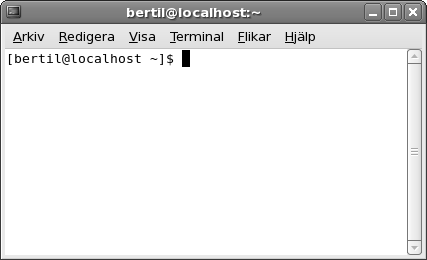
\includegraphics[width=.8\textwidth]{pics/bertil.png}
\xcaption{Användaren ''bertil'' inloggad på datorn ''localhost'', i hemmappen.}
\end{figure}

Så kan kommandoprompten se ut:

\xcode{användarnamn@datornamn:aktuell\_mapp\$}

Exempel:

\xcode{bertil@skalman:\texttildelow{}/dokument\$}

Detta betyder kort och gott att den aktuella användaren heter ''bertil'', att datornamnet är ''skalman'' och att du för tillfället befinner dig i mappen ''dokument'', som ligger i din hemmapp. Det lilla tecknet \xdefinitionstyle{\xoption{\texttildelow{}}}\index{specialtecken!\xoption{\texttildelow{}} (tilde)} är ett alias för den aktuella användarens hemmapp (mer om detta i \secref{sec:tilde}). Sist i prompten är ett dollartecken, \xdefinitionstyle{\$}\index{användare!\$ (vanlig användare)}, som anger att den aktuella användare är en vanlig användare utan administrationsrättigheter. Om du är inloggad som administratören på en dator, med root-användaren, anges detta med ett brädgårdstecken, \xdefinitionstyle{\#}\index{användare!\# (root-användaren)}\index{root} (läs mer i \secref{sec:rootanvandaren}).

\subsection{Skriva in kommandon}

Det är enkelt att skriva in och köra ett kommando. Skriv helt enkelt kommandonamnet efter prompten, lägg till eventuella \xdefinition{alternativ} som kommandot stöder och avsluta med eventuella \xdefinition{argument}. Alternativ ändrar beteendet hos kommandot, argumentet är det som kommandot ska köras på (exempelvis en fil, sökväg eller text).

Skriv kommandon på följande sätt, avsluta alltid med ett tryck på tangenten \xkey{enter}:

\xcode{kommandonamn -alternativ argument}

Detta gäller bokens alla kommandon, även om tangenttryckningen på \xkey{enter} har uteslutits från instruktionerna för att undvika onödiga upprepningar.

Ett praktiskt exempel:

\xcode{ls -l /home/bertil}

Detta kör kommandot \xcommand{ls} med alternativet \xoption{-l} och argumentet \xargument{/home/bertil}, vilket visar en utförlig lista med alla filer i hemmappen för användaren ''bertil''. Läs mer om \xcommand{ls} i \cmdref{cmd:ls}.

\begin{figure}[ht]
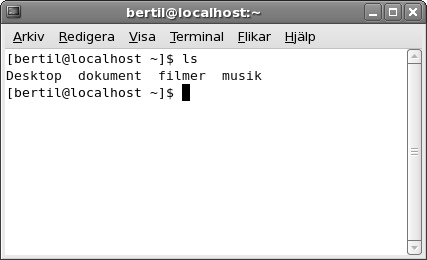
\includegraphics[width=.8\textwidth]{pics/bertil-ls.png}
\xcaption{Resultatet av kommandot \xcommand{ls}: innehållet i ''bertils'' hemmapp.}
\end{figure}

För att ange flera alternativ till ett kommando på en och samma gång går det lika bra att slå ihop dem som att ange dem separerade från varandra.

Till exempel fungerar 

\xcode{ls -al /home/bertil}

precis lika bra som 

\xcode{ls -a -l /home/bertil}

I vissa fall använder olika kommandon samma alternativ med samma betydelse, men huvudregeln är att varje kommando har en unik uppsättning alternativ. För en del kommandon kan alternativ inte anges alls. 

\xnote{Lägg märke till att alternativ ibland kallas 'flagga'\index{flagga|see{alternativ}} eller 'väljare'\index{väljare|see{alternativ}}. Dessa ord är alla synonymer i kommandoradssammanhang.}

\subsection{Undvik root-användaren}\label{sec:rootanvandaren}

Kör kommandona i den här boken som en vanlig användare, inte som systemadministratören \xuser{root}. Detta gäller särskilt dig som är nybörjare och experimenterar mycket. Om du är inloggad som en vanlig användare kan du inte oavsiktligen ställa till med problem på systemet -- datorn låter dig inte göra det. Som root-användaren har du däremot oinskränkt makt över minsta del av datorn. Om du som root-användare av misstag skriver fel kan det få onödigt tråkiga konsekvenser.

Vissa kommandon måste köras som root-användaren för att fungera. Detta anges i sådana fall tydligt.

I Bash ser du om du är inloggad som en vanlig användare genom att prompten avslutas med ett dollartecken, \xdefinitionstyle{\$ (vanlig användare)}. Om du är inloggad som root-användaren visas detta med tecknet \xdefinitionstyle{\# (root-användaren)}.

Exempel:

\xcode{root@skalman:\texttildelow{}\#}

\xtip{Om du under läsningen av den här boken vill experimentera med olika kommandon och inställningar på datorn kan du skapa skapa en särskild testanvändare på datorn. Då lämnar du din riktiga hemmapp i fred, och kan experimentera utan att oroa dig. Se \cmdref{cmd:adduser} och \cmdref{cmd:su} för mer information.}

\subsubsection{Använd sudo}\label{sec:sudo}

I vissa operativsystem är root-användaren helt inaktiverad. Detta gäller exempelvis i Mac~OS~X och Ubuntu Linux. Istället kan vanliga användare tillfälligt få root-rättigheter genom att skriva in kommandot \xcommand{sudo} före det önskade kommandot. 

Kommandosyntax:

\xcode{sudo kommandonamn}

Om du är systemadministratör på datorn ger \xcommand{sudo} dig rätt att köra det önskade kommandot, annars talar \xcommand{sudo} om för dig att du inte har rätt att köra kommandot.

Mer information om kommandot finns i \cmdref{cmd:sudo}.

\subsection{exit}\label{sec:exit}

Avslutar ditt skal (vilket oftast leder till att den virtuella terminalen stängs). 

Exempel:

\xcode{exit}

\xtip{Du kan också använda \xkeycombination{\xkey{ctrl}+\xkey{d}} eller kommandot \xcommand{logout} för att logga ut ur ett inloggningsskal.}

\subsection{Grundläggande kommandon}

Börja gärna med att ta en närmare titt på följande kommandon om du är nybörjare och vill komma igång med att utforska systemet.

\begin{description}

\item[\xcommandstyle{ls}] Se \cmdref{cmd:ls}.
\item[\xcommandstyle{cd}] Se \cmdref{cmd:cd}.
\item[\xcommandstyle{cp}] Se \cmdref{cmd:cp}.
\item[\xcommandstyle{mv}] Se \cmdref{cmd:mv}.
\item[\xcommandstyle{rm}] Se \cmdref{cmd:rm}.
\item[\xcommandstyle{mkdir}] Se \cmdref{cmd:mkdir}.
\item[\xcommandstyle{rmdir}] Se \cmdref{cmd:rmdir}.
\item[\xcommandstyle{find}] Se \cmdref{cmd:find}.

\end{description}

\section{Specialtecken och jokertecken}\label{sec:joker}

Det finns ett antal specialtecken som du behöver känna till när du jobbar med skalet. Dessa specialtecken och jokertecken fungerar med alla kommandon som du kör i skalet.

\subsection{. (punkt)}

En punkt betyder kort och gott ''här''. Den anger med andra ord den aktuella mappen.

Om du till exempel står i mappen ''/home/bertil'' och vill kopiera en fil till just den här mappen kan du använda kommandot \xcommand{cp} (kortform av \xeng{copy}, se \cmdref{cmd:cp}).

\xcode{cp /tmp/fil.txt .}

istället för

\xcode{cp /tmp/fil.txt /home/bertil}

Båda exemplen ovan kopierar ''fil.txt'' från mappen ''/tmp'' till den mapp du för tillfället står i, men den övre är enklare och snabbare.

\subsection{.. (två punkter)}

Två punkter anger föräldramappen. Du använder två punkter för att ange en mapp i hierarkin (närmare roten i filträdet). 

Om du till exempel står i mappen ''/home/bertil'' och vill gå till ''/home'' kan du använda kommandot \xcommand{cd} (kortform av \xeng{change directory}, se \cmdref{cmd:cd}) med två punkter som argument:

\xcode{cd ..}

Detta ställer dig i mappen ''/home''.

Om du står i mappen ''/home/bertil/musik/mp3'' och vill hoppa till ''/home/bertil/dokument'' kan du skriva

\xcode{cd ../../dokument}

Om du står i mappen ''/home/bertil/dokument'' och vill se en detaljerad lista över filerna i ''/home/bertil'' kan du använda kommandot \xcommand{ls} (kortform av \xeng{list}, se \cmdref{cmd:ls}).

\xcode{ls -l ..}

\subsection{\texttildelow{} (tilde)}\label{sec:tilde}

Tilde-tecknet används som ett alias för användarens hemmapp.

Om ditt användarnamn till exempel är ''bertil'' kan du istället för att skriva in \xcommandstyle{cd /home/bertil} helt enkelt knappa in \xcommandstyle{cd \texttildelow{}}. Om du vill hoppa till en mapp i hemmappen som heter dokument kan du skriva \xcommandstyle{cd \texttildelow{}/dokument}.

\xtip{\texttildelow{} (tilde) kan också användas som en genväg till andra användarens hemmappar. Skriv då \texttildelow{}användarnamn, så hoppar du till hemmappen för den användaren.}

\subsection{? (frågetecken)}

\index{jokertecken!\xoption{?} (frågetecken)}

Jokertecknet ? representerar ett enda tecken, vilket som helst. Till exempel matchar ''hd?'' både hda, hdb, hdc eller vilket annat tecken som helst från a till z, liksom vilken siffra som helst mellan 0 till 9.

Exempel:

\xcode{ls dokument-?.doc}

Detta visar alla filer i den aktuella mappen vars namn börjar med ''dokument-'', som därefter innehåller exakt ett tecken (vilket som helst) och som slutar med ''.doc''.

Läs mer om hur du kan använda detta jokertecken i skalet, eller för att skapa reguljära uttryck i olika program, i \charef{cha:regexp}.

\subsection{* (asterisk)}

\index{jokertecken!\xoption{*} (asterisk)}

Detta är det vanligast förkommande jokertecknet, med betydelsen matcha allt. Asterisken representerar ett godtyckligt antal tecken (inklusive inget tecken alls). Till exempel matchar ''cd*'' både cd, cda, cdrom, cdrecord -- allt som börjar med cd inklusive enbart cd. Exemplet ''m*l'' matchar både ml, mall och multilateral -- allt som börjar med m och slutar med l, med andra ord.

Exempel:

\xcode{ls *.doc}

Detta visar alla filer som slutar med ändelsen .doc i den aktuella mappen.

Läs mer om hur du kan använda detta jokertecken i skalet, eller för att skapa reguljära uttryck i olika program, i \charef{cha:regexp}.

\subsection{\textbackslash{} (bakstreck)}\label{sec:backslash}

Tecknet \textbackslash{} kan användas före speciella tecken som mellanslag och jokertecken för att förhindra att Bash försöker tolka, ''expandera'', dem. Om du ber skalet utföra något på en fil eller mapp som i sitt namn innehåller ett specialtecken kan du använda bakstrecket för att skydda det från att först tolkas av skalet.

Ett sådant speciellt tecken är mellanslag. Du kan byta till en mapp vars namn innehåller mellanslag så här:

\xcode{cd namn\textbackslash{} med\textbackslash{} mellanslag}

Utan bakstrecken skulle ovanstående inte fungera eftersom skalet Bash skulle försöka byta till en mapp med endast namnet ''namn'' (resten av raden skulle ignoreras).

%Tecken som behöver beskydd av bakstrecket är \begin{verbatim}^[]$()|*?{}\\end{verbatim}

\xtip{Istället för att använda bakstreck före mellanslag i filnamn kan du kapsla in hela filnamnet med enkla citationstecken.

Exempel:

\xcode{cd \textquotesingle{}namn med mellanslag\textquotesingle{}}

Båda sätten fungerar lika bra!

}

\xnote{Lägg märke till att \xkeycombination{\xkey{tab}}-tangenten (automatisk ifyllning av namn och kommandon) automatiskt använder bakstreck före mellanslag, du slipper skriva in dem manuellt.}

\section{Redigera kommandon}

\subsection{Komplettera automatiskt}

Skriv in de första bokstäverna i namnet på ett kommando och tryck på tangenten \xkeycombination{\xkey{tab}}, så kompletterar Bash automatiskt med det som återstår av namnet åt dig. Du kan använda funktionen för att fylla i kommandonamn (\xeng{automatic commmand completion}), liksom när du navigerar och jobbar i filsystemet, exempelvis när du hoppar mellan mappar, kopierar filer och så vidare (\xeng{automatic filename completion}).

\subsection{Tangentbordsgenvägar}

Det finns många tangentbordsgenvägar i GNU/Linux som du kan använda för att förenkla redigeringen av kommandon i skalet och för att snabba upp arbetet. Nedan är en lista med några av dem (se också \xkeycombination{\xkey{ctrl}+\xkey{r}} i sektionen om kommandoradshistoriken).

\subsubsection{CTRL+A och CTRL+E}

Dessa tangentbordsgenvägar används för att gå till början eller slutet av en rad i terminalen. Använd \xkeycombination{\xkey{ctrl}+\xkey{a}} för att gå till början på raden, använd \xkeycombination{\xkey{ctrl}+\xkey{e}} för att hoppa till slutet av raden.

Normalt fungerar tangenterna markerade \xkeycombination{\xkey{home}} och \xkeycombination{\xkey{end}} likadant om du är van vid dessa.

\subsubsection{CTRL+K}

Den här tangentbordsgenvägen används för att klippa ut eller radera det som finns framför markören.

\subsubsection{CTRL+Y}

Den här tangentbordsgenvägen kan användas för att klistra in det du senaste klippte ut (med \xkeycombination{\xkey{ctrl}+\xkey{k}} eller \xkeycombination{\xkey{ctrl}+\xkey{w}}).

\subsubsection{CTRL+W}

Den här tangentbordsgenvägen kan användas för att klippa ut eller radera hela ord.

\subsection{Kommandoradshistoriken}

Alla kommandon du skriver in sparas av Bash. Du kan bläddra bland de kommando du har skrivit tidigare genom att trycka på uppåtpil- och nedåtpil-tangenterna på tangentbordet. Tryck \xkeycombination{\xkey{enter}} för att utföra ett kommando du har bläddrat fram till, eller använd vänsterpil- och högerpil-tangent\-erna för att redigera kommandot. 

Du kan också använda det i Bash inbyggda kommandot \xcommand{history}. Med kommandot kan du visa alla kommandon du har använt. Använd det så här:

\xcode{history n}

Detta skriver ut de senaste n (där n står för godtyckligt antal) kommandona. Skriv in \xcommand{history} (utan alternativ) för att se hela historiklistan.

Du kan också skriva in \xcommandstyle{!n} för att köra kommando nummer n. Använd \xcommandstyle{!!} för att köra det senaste inskrivna kommandont.

\xcommandstyle{!-n} kör kommandot n steg bakåt i listan (därmed blir \xcommandstyle{!-1} samma sak som \xcommandstyle{!!}).

\xcommandstyle{!sträng} kör de senaste kommandot som börjar med texten ''sträng'' (där sträng betyder godtycklig text, kan vara vad som helst) och \xcommandstyle{!?sträng?} kör de senaste kommandot som innehåller ordet ''sträng''. Exempel:

\xcode{!cd}

Kör det senaste kommandot du skrev in som börjar med \xcommand{cd}.

''kommandonamn !*'' kör ''kommandonamn'' med de argument du använde med ditt förra kommando. Detta är användbart när du stavar kommandonamnet fel, till exempel. Om du skrev:

\xcode{emasc /home/bertil/program.java /tmp/test.java}

för att använda Emacs för att öppna de två angivna filerna kommer du misslyckas eftersom kommandonamnet är felstavat. Om du då skriver:

\xcode{emacs !*}

kommer du köra emacs med de argument du senaste skrev in på kommandoraden. Det är med andra ord detsamma som:

\xcode{emacs /home/bertil/program.java /tmp/test.java}

Använd \xkeycombination{\xkey{ctrl}+\xkey{r}} för att göra en bakåtvänd sökning i historiken, \xeng{reverse-i-search}. Om du till exempel upprepa det du skrev in senaste gången du använd kommandot \xcommand{snort} skriver du:

\xcode{\xkeycombination{\xkey{ctrl}+\xkey{r}} snort}

Då ser du följande i terminalfönstret:

\xcode{(reverse-i-search)\textasciigrave{}\textquotesingle{}:}

Skriv in det du söker och använd sedan \xkeycombination{\xkey{ctrl}+\xkey{r}} för att bläddra bakåt bland sökträffarna i historiken.

Tryck \xkeycombination{\xkey{ctrl}+\xkey{r}} så många gånger du behöver för att hitta det du söker. Tryck då \xkeycombination{\xkey{enter}} för att köra kommandot.

Du kan också använda högerpil- och vänsterpil-tan\-gen\-ter\-na för att åter sätta in kommandot på kommandoraden, så att du kan redigera det.

\chapter{Söka hjälp}\index{hjälp!om kommandon}

\xintro{Det här kapitlet ger information om hur du söker hjälp i ett GNU/Linux-system. Det finns nästan alltid någon form av bra hjälp för verktygen på datorn.}

\section{-?, -h, -{}-h, -{}-help}

Pröva alternativen \xoption{-?}, \xoption{-{}-h}, \xoption{-{}-help} och \xoption{-h} med ett kommando. 

Exempel:

\xcode{ls -{}-help} 

Nästan alla kommandon visar översiktligt information om dess användning med något av dessa alternativ. Tyvärr finns det ingen enhetlig standard kring vilket av alternativen som används, utan du måste pröva dig fram. Det är ofta värt besväret -- den inbyggda hjälpen brukar vara mer kortfattad än den som du kan se med \xcommand{man} eller \xcommand{info}, så det är en bra idé att börja med den.

\section{man}\index{hjälp!kortfattad med man}

\xcommandinfo{man}{Visar manual-sidor för program}{man\xstandard}{man\xstandard}{man\xstandard}{man man}{\$}

Detta kommando visar kortfattad information om ett program från det inbyggda manualsystemet på datorn.

Kommandosyntax:

\xcode{man programnamn}

Pröva till exempel att läsa manual-sidan för \xcommand{man} (det vill säga \xcommand{man}-kommandots egen man-sida):

\xcode{man man}

Observera att manual-sidorna i allt väsentligt endast finns tillgängliga på engelska, även om vissa sidor har översatts till svenska.

\xnote{Stäng ned manual-visaren med tangenten \xkeycombination{\xkey{q}}.}

Manual-sidorna är indelade i flera så kallade sektioner, från 1--9. Vissa kommandon har endast en manual-sida, andra har flera i olika sektioner. Du kan använda kommandot \xcommand{apropos} (\cmdref{cmd:apropos}) för att ta reda på vilka sektioner du ska kolla i. 

Indelningen i sektioner ser ut så här:

\begin{enumerate}

\item kommandon
\item systemanrop (för programmerare)
\item funktioner (för programmerare)
\item enhetsfiler under \xfile{/dev}
\item filformat
\item spel
\item diverse
\item admin-kommandon
\item linuxkärnan (för programmerare)

\end{enumerate}

En man-sida med ett visst namn kan finnas i flera sektioner samtidigt. Ibland kan du se referenser till mansidor med tillhörande sektion inom parentes. Till exempel refererar ''time(1)'' till ls-manualen i sektion 1.

Syntaxen för att se manual-sidan i en viss sektion är:

\xcode{man sektionsnummer programnamn}

Exempel:

\xcode{man 7 time}

Detta visar man-sidan i sektion 7 för kommandot \xcommand{time}, innehållet i sektion 1 är helt annorlunda.

\xcode{man -k sträng}

Du kan också söka efter en sträng (godtycklig text) i alla manualsidor. Då frågar programmet om du vill se varje sida som det hittar. Omgärda strängen du söker efter med dubbla citattecken '' och '' om den innehåller mellanslag.

\xwarning{Observera att sökningen tar mycket, mycket lång tid, eftersom programmet söker efter strängen i \textit{alla} man-sidor på datorn.}

\xcode{man -f kommando}

Detta visar uppgifter om kommandot. För att det ska fungera måste root-användaren på datorn först köra kommandot \xcommand{makewhatis}. 

\xnote{\xcommandstyle{man -f kommando} ger samma resultat som att använda kommandot \xcommand{whatis} (se nedan).}

\section{info}\index{hjälp!detaljerad med info}

\xcommandinfo{info}{Visar info-sidor för program}{info\xstandard}{info\xstandard}{info\xstandard}{man info, info info}{\$}

Visar en mer detaljerad manual med hyperlänkar om ett visst kommando. Detta fungerar endast med vissa kommandon.

Kommandosyntax:

\xcode{info programnamn}

\section{whatis}\index{hjälp!beskrivning av program}

\xcommandinfo{whatis}{Visar korta beskrivningar av program}{man-db\xstandard}{man\xstandard}{man-db\xstandard}{man whatis}{\$}

Visar en enradsbeskrivning om programmet. Programnamnet måste skriva in exakt, annars visas ingenting alls. Använder sig av whatis-databasen (se nedan).

Kommandosyntax:

\xcode{whatis programnamn}

\xcode{makewhatis}

Skapar den så kallade whatis-databasen som kommandona \xcommand{apropos}, \xcommand{whatis} och \xcommandstyle{man -f} behöver. Efter att databasen en gång har skapats behöver kommandot inte köras igen.

\xnote{Observera att kommandot måste köras av root-användaren, och att det tar ganska lång tid att skapa databasen.}

\section{apropos}

\xcommandinfo{apropos}{Söker efter beskrivningar och namn i manual-sidor}{apropos\xstandard}{apropos\xstandard}{man\xstandard}{man apropos}{\$}

\xcode{apropos}

Söker i whatis-databasen efter strängar, på likande sätt som \xcommand{whatis}, men med den skillnaden att det söker efter och skriver ut alla resultat som matchar strängen (eller en del av strängen). Kommandot behöver en whatis-databas för att fungera (se ovan).

Kommandosyntax:

\xcode{apropos sträng}

\xnote{Att köra kommandot \xcommand{apropos} ger samma resultat som \xcommandstyle{man -k}.}

\section{Ytterligare källor till hjälp}

Utöver de vanligaste hjälp- och dokumentationskällorna \xcommand{man}, \xcommand{info} och den inbyggda hjälpen i kommandon finns det information att hämta på några ställen till.

Till exempel kan det under \xfilestyle{/usr/share/doc/paketnamn} finnas ytterligare information att hitta, exempelvis HTML-format. Dessa sidor kan du titta på med en webbläsare.

För kommandon som är inbyggda i skalet Bash kan man se hjälptexter med hjälp av \xcommand{help kommandonamn} direkt vid kommandoprompten.\index{hjälp!om Bash-kommandon}. Om du vill veta om ett kommando är inbyggt i skalet eller är ett eget program kan du köra kommandot \xcommand{type} följt av kommandots namn (se \cmdref{cmd:type}).

Dessutom finns en uppsjö dokumentation på nätet, som är enkelt åtkomlig tack vare sökmotorer.


\chapter{Skal- och miljövariabler}\label{cha:variables}

\xintro{Det är tack vare en miljövariabel som du kan starta ett program bara genom att skriva dess namn, utan att känna till i vilken mapp det ligger. Miljövariabler har också många andra användningsområden.}

\index{miljövariabel|(}
\index{skalvariabel|(}

När skalet startas läser det in så kallade \xdefinitionstyle{miljövariabler}\index{miljövariabel} i datorns minne som olika kommandon och program kan använda sig av. Varje miljövariabel innehåller ett visst värde, som kan vara exempelvis information om standardspråk på datorn, sökvägen till körbara program och kommandon, sökvägen till användarens hemmapp och så vidare (se nedan för en lista med exempel). 

Så fort ett program behöver kolla upp sökvägen till den aktuella användarens hemmapp kan det kontrollera miljövariabeln \xenv{HOME}.

Det är miljövariabeln \xenv{PATH} som håller reda på sökvägen till mappar som innehåller körbara program och kommandon. Det är denna miljövariabel som gör det möjligt för Bash att hitta hela sökvägen till och starta ett kommando, exempelvis \xfilestyle{/bin/ls} när du skriver \xcommand{ls}. Hade det inte varit för att variabeln \xenv{PATH} innehöll sökvägen \xfilestyle{/bin} hade Bash inte hittat kommandot alls (du hade då behövt ange \xfilestyle{/bin/ls} för att köra det).

Som namnet \textit{variabel} antyder kan värdet av en miljövariabel fritt ändras av användaren. En användare eller ett program kan dessutom själv skapa valfria egna miljövariabler när som helst.

Miljövariabler går i arv. Nya processer som skapas i skalet (exempelvis när du kör ett kommando) får tillgång till samma variabler som skalet, som därmed kan sägas vara \textit{förälderprocess} till alla andra processer som startas i det. Däremot kan en föräldraprocess inte ärva miljövariabler i andra riktningen, från en \xdefinitionstyle{barnprocess}.

Här är några vanliga miljövariabler på datorn:

\begin{description}
\item[\xenv{PATH}] anger de sökvägar skalet letar i efter körbara program/kommandon
\item[\xenv{HOME}] anger sökvägen till användarens hemmapp
\item[\xenv{TERM}] anger vilken terminal eller virtuell terminal som används
\item[\xenv{PS1}] anger hur kommandoprompten ser ut
\end{description}

Vanligtvis läser Bash in standarduppsättningen med variabler från filen \xfile{\texttildelow{}/.bashrc} (i användarens hemmapp) när skalet startar. (Punkten framför namnet indikerar att filen är osynlig, läs mer om hur du visar sådana filer i \cmdref{cmd:ls}.)  Om du vill att en miljövariabel ska finnas kvar när du startar skalet efter omstart lägger du till miljövariabeln på en tom rad i filen \xfile{\texttildelow{}/.bashrc} i din hemmapp. Om du önskar att miljövariabeln ska fungera för alla användare på datorn kan du lägga till den till filen \xfile{/etc/profile}.

\section{export}\index{miljövariabel!export}

\xcommandinfo{export}{Exporterar en skalvariabel till en miljövariabler}{bash\xstandard}{bash\xstandard}{bash\xstandard}{man bash}{\$}

Du kan skapa eller ändra en befintlig variabel i ditt Bash-skal på den här formen:

\xcode{VARIABEL=värde}

Exempel:

\xcode{FAVORITMAT=hamburgare}

Ännu så länge finns variabeln endast i det aktuella skalet. Om du vill göra denna \xdefinition{skalvariabel} till \xdefinition{miljövariabel} använder du kommandot \xcommand{export}.

Kommandosyntax:

\xcode{export VARIABEL}

Exempel:

\xcode{export FAVORITMAT}

Genom att exportera skalvariabeln har du skapat en miljövariabel. Använd kommandot \xcommand{printenv} för att se värdet av miljövariabeln.

\xtip{Du kan göra båda operationerna ovan i ett svep. Om du skriver

\xcode{export FAVORITMAT=hamburgare} 

skapas miljövariabeln i ett steg.}

Nu kanske variabeln \xenvstyle{FAVORITMAT} inte är så särskilt användbar, men nedanstående exempel kan komma till större användning.

Miljövariabeln \xenv{PATH} består av en lista med mappar som innehåller körbara filer. Sökvägarna skiljs åt med ':', kolon. Om du själv har installerat ett program på datorn i en mapp som inte finns i miljövariablen \xenv{PATH}, exempelvis i mappen \xfilestyle{/home/bertil/program}, kan du lägga till den till listan genom att skriva följande:

\xcode{export PATH=\$PATH:/home/bertil/program}

Detta lägger till den privata programmappen till slutet av listan med sökvägar i den befintliga variablen \xenv{PATH}. \xenv{PATH} innehöll sökvägarna \xfilestyle{/bin:/usr/bin:/usr/local/bin}  tidigare innehåller den efter att du har kört ovanstående \xfilestyle{/bin:/usr/bin:/usr/local/bin:/home/bertil/program}.

Alla program du installerar i den privata programmappen kan du starta genom att skriva kommandonamnet, utan att ange hela sökvägen.

Om du vill ändra utseendet på kommandoprompten från standardutseendet till något kompaktare kan du testa att köra följande:

\xcode{export PS1=\textquotedbl{}\textbackslash{}u \textbackslash{}\$ \textquotedbl{}}

Detta ändrar prompten så att den enbart innehåller användarnamnet följt av dollartecken.

Om du vill göra en miljövariabel permanent lägger du till den till filen \xfile{\texttildelow{}/.bashrc} i din hemmapp.

\section{printenv}\index{miljövariabel!printenv}

\xcommandinfo{printenv}{Visar en eller flera miljövariabler}{coreutils\xstandard}{coreutils\xstandard}{coreutils\xstandard}{man printenv}{\$}

Använd \xcommand{printenv} för att se värdet av en specifik eller alla miljövariabler.

Kommandosyntax:

\xcode{printenv miljövariabel}

Exempel:

\xcode{printenv HOME}

Detta visar vilken som är användarens hemmapp.

\xcode{printenv}

Detta visar alla miljövariabler.

\xnote{Du kan även använda kommandona \xcommand{env} och \xcommand{set} (se \cmdref{cmd:set}) för att se miljövariabler och deras värden. Med dessa två kommandon kan du också ställa in miljövariabler.}

\index{miljövariabel|)}
\index{skalvariabel|)}

\chapter{Knep och tips}

\xintro{Det här kapitlet innehåller ett antal knep som gör tiden framför kommandoraden lite effektivare och säkrare.}

\section{alias}

\xcommandinfo{alias}{Sätta alias för kommandon i Bash}{bash\xstandard}{bash\xstandard}{bash\xstandard}{man bash}{\$}

Ett alias är ett annat namn för ett kommando. Du kan ställa in dina alias för att exempelvis använda ett eller flera extraalternativ, eller helt förändra beteendet för ett kommando. Du kan ställa in dina alias under en pågående session med hjälp av alias-kommandot eller permanent i filen \xfile{\texttildelow{}/.bashrc} i din hemmapp.

Alias-kommandot (som är inbyggt i Bash) visar dina aktuella alias. 

\xcode{alias}

Detta visar alla alias som du använder för närvarande. Många distributioner ställer in ett antal alias från början, så det är en god idé att köra kommandot för att se vilka de är.

Du kan använda kommandot \xcommand{unalias} för att ta bort ett alias. Du kan temporärt inaktivera av ett alias genom att lägga till ett \textbackslash{} (bakstreck) framför kommandot (se nedan). Då körs originalkommandot istället för aliaset.

Exemplet nedan visar hur en alias-sektion i din \xfile{\texttildelow{}/.bashrc}-fil kan se ut:

\begin{verbatim}
# fråga innan filer skrivs över, 
# ange var filerna kopieras
alias cp='cp -vi'

# fråga innan borttagning
alias rm='rm -i'

#fråga innan filer skrivs över vid flyttning
alias mv='mv -i'
\end{verbatim}

Du kan när som helst lägga till valfritt antal alias i filen. Nytillagda rader blir aktiva nästa du startar ett skal. Du kan
alltså enkelt testa dina ändringar genom att öppna en ny terminal.

Tecknet bakstreck används för att köra ett kommando och förbigå eventuella alias.

Om \xcommand{rm} exempelvis görs till ett alias för \xcommandstyle{rm -i} blir resultatet körs \xcommandstyle{rm -i} varje gång du skriver \xcommand{rm}.

Men om du skriver \xcommandstyle{\textbackslash{}rm} ignorerar skalet aliaset och kör \xcommand{rm}, precis som du skrev in det. Då kommer kommandot inte fråga dig om du verkligen vill radera det du kör kommandot på.

Tänk på att aliaset för ta-bort-kommandot rm finns av en anledning. Om du använder kommandot oförsiktigt kan du råka radera filer som du inte vill ta bort.

Använd därför endast \xcommandstyle{\textbackslash{}rm} om du vet vad du gör. Det är inte helt enkelt att återskapa raderade filer, \xcommand{rm} raderar direkt utan att först lägga filerna i en papperskorg.

Läs mer om \textbackslash{} i \secref{sec:backslash}.


\section{set}\index{miljövariabel!set}

\xcommandinfo{set}{Läs och sätt variabler i Bash}{bash\xstandard}{bash\xstandard}{bash\xstandard}{man bash}{\$}

\xcommand{set} är ett av de många inbyggda kommandona som finns i Bash. 

Om du anger alternativet \xoption{-x} skriver Bash ut namnet på det kommando som kommer att köras, precis innan det körs. 

Detta är användbart när du vill förstå exakt vad som händer med vissa kommandon, exempelvis om det innehåller jokertecken eller speciella tecken som orsakar problem, eller krångliga alias. 

Exempel: 

\xcode{set -x}

Detta säger åt Bash att slå på funktionen att visa exakt vad som körs när du skriver in ett kommando. Om du till exempel skriver \xcommand{ls} skriver skalet ut \xcommandstyle{+ ls -F -{}-color=auto} innan det körs (exakt vad som visas beror på vilka alias, om något, som används på ditt system).

Detta betyder att kommandot egentligen är ett alias för \xcommand{ls} med alternativen \xoption{-F} och \xcommandstyle{-{}-color=auto}. 

Använd \xcommandstyle{set +x} för att stänga av funktionen.

Kör kommandot \xcommand{help set} för att se information om kommandots många alternativ, eller läs i Bash-manualen.

\section{echo}

\xcommandinfo{echo}{Visar det du just skrev in i terminalen}{bash\xstandard}{bash\xstandard}{coreutils\xstandard}{help echo}{\$}

Ett litet kommando som visar sina argument i terminalen.

Exempel:
	
\xcode{echo \textquotedbl{}hej världen\textquotedbl{}}

Då visas ''hej världen'' i terminalen.

Pröva även alternativet \xoption{-e}. Då kan du använda escape-tecken, \textbackslash{} (bakstreck) tillsammans med vissa tecken för att formatera visningen på skärmen. Exempel: \xcommandstyle{\textbackslash{}t} för tabulator, \xcommandstyle{\textbackslash{}n} för ny rad.

Exempel:

\xcode{echo -e \textquotedbl{}hej\textbackslash{}n hopp\textbackslash{}n nytt\textbackslash{}t hopp\textquotedbl{}}

Ett användningsområde för \xcommand{echo} är att förebygga olyckor. Genom att skriva in \xcommand{echo} följt av det eller de kommandon du vill köra kan du undvika att råka ut för något du inte hade tänkt dig. Med \xcommand{echo} ser du också hur jokertecken expanderar, vilket gör att du förstår exakt vad som händer innan du faktiskt kör kommandot.

Exempel:

\xcode{echo rm -R *}

Detta skriver ut vad som skulle ha raderats om du hade kört \xcommand{rm}-kommandot med argumentet \xargument{*}. Om du sätter \xcommand{echo} före ett kommando gör du det harmlöst (det expanderar endast eventuella jokertecken så att du ser vad som annars skulle ha skett).

\section{script}

\xcommandinfo{script}{''Spelar in'' allt som visas i skalet}{bsdutils\xstandard}{util-linux\xstandard}{bsdutils\xstandard}{man script}{\$}

Kommandot \xcommand{script} skapar en avskrift av en hel skalsession. Kommandot skriver en kopia av din session till en fil, inklusive kommandon du skriver och resultatet av dem.

Aktivera inspelningen genom att skriva \xcommand{script}. Avbryt inspelningen genom att skriva \xcommand{exit}.

Som standard sparas avskriften i en fil med namnet \xfile{typescript} i den mapp du stod i när du startade \xcommand{script}.

\section{reset}\index{återställa terminalen}

\xcommandinfo{reset}{Intialisera terminalen}{ncurses-bin\xstandard}{ncurses\xstandard}{ncurses-bin\xstandard}{man reset}{\$}

\xcommand{reset}-kommandot nollställer den aktuella terminalen. Det är användbart om ett program gör att texten i din terminal blir konstig. Skriv in kommandot, så fixar det saken.

Exempel:

\xcode{reset}

\section{init=/bin/sh}

\index{init!\xfilestyle{init=/bin/sh}}
 
Om du någon gång råkar ut för att du inte kan starta och logga in på din dator kan du genskjuta den normala startsekvensen och logga in med skalet \xcommand{sh} på datorn (som är mindre och lättare än Bash), innan några andra program och processer hinner starta. Du kan göra detta genom att ge argumentet \xargument{init=/bin/sh} till systemet innan det startar.

De flesta Linuxdatorer använder startladdaren (\xeng{boot loader}) GRUB, och du kan redigera startargumenten i GRUB om du trycker ned \xkey{esc}-tangenten precis när GRUB laddas i samband med datorstart.

\chapter{Installera program}\label{cha:installera}

\xintro{Det här kapitlet hjälper dig igång med de två vanligaste kommandoradsverktygen för att ladda ned och installera program i binärformat.}

Kommandona nedan hjälper dig att snabbt och smidigt installera färdigkompilerade versioner av många av bokens kommandon på din dator.

\section{apt-get (Debian, Ubuntu, Fink)}

\xnote{Detta avsnitt gäller dig som har en Debian Linux-dator, eller använder en Debian- och dpkg-baserad, exempelvis Ubuntu. Avsnittet är också relevant för dig som använder Fink i Mac~OS~X.\index{Fink}\index{Mac~OS~X}}

Det bakomliggande pakethanteringssystemet i Debian Linux kallas dpkg (\xeng{Debian package management system}). Utöver dpkg, som bland annat innehåller en databas över alla tillgängliga och installerade program (och beroenden mellan olika paket) finns ett antal verktyg för att enkelt och smidigt ladda ned, kontrollera och installera paket i det så kallade deb-formatet på datorn.

Det vanligaste kommandoradsverktyget för att hantera dpkg kallas \xcommand{apt-get}. Verktyget är standard i Debian och Debian-baserade distributioner som exempelvis Ubuntu. 

Om du använder Mac~OS~X kan du med hjälp av Fink-projektet också använda \xcommand{apt-get} för att hantera installation av UNIX-verktyg i binärformat på Macen. Instruktioner för hur du kommer igång med Fink finns på projektet hemsida, \url{http://fink.sourceforge.net}.

\subsection{apt-get}\index{program!installera}\index{installera program}

\xcommandinfo{apt-get}{Pakethanterare för kommandoraden}{apt\xstandard}{apt}{bsdutils\xstandard}{man apt-get}{\#}

\xcommand{apt-get} laddar ned paket direkt från servrar på nätet, så kallade förråd (\xeng{repository}). Vilka förråd som är aktiva styrs av innehållet i filen \xfile{/etc/apt/sources.list}.

Kommandot måste köras som root-användaren (eller genom att använda \xcommand{sudo}) och kräver en fungerande internetuppkoppling eller tillgång till ett paketförråd exempelvis på cd-skiva för att fungera.

\subsubsection{Kontrollera om det finns uppdaterade paket}\index{program!uppdatera}\index{uppdatera program}

Kommandonsyntax för uppdatering av paketlistor i aktiverade förråd:

\xcode{sudo apt-get update}

\subsubsection{Installera nya versioner av alla uppdaterade paket}

Kommandosyntax:

\xcode{sudo apt-get dist-upgrade}

Detta laddar ned och installerar alla uppdaterade paket som finns tillgängliga i paketförråden.

\subsubsection{Installera ett nytt paket}

Kommandosyntax:

\xcode{sudo apt-get install paketnamn}

Exempel:

\xcode{sudo apt-get install wget}

Detta laddar automatiskt ned, installerar och konfigurerar programmet \xcommand{wget}, med hjälp av \xcommand{sudo} körs kommandot med administratörsrättigheter.

\subsubsection{Ta bort ett paket}\index{program!avinstallera}\index{avinstallera program}

Du kan också använda \xcommand{apt-get} för att ta bort paket från datorn.

Exempel:

\xcode{sudo apt-get remove wget}

Detta avinstallerar \xcommand{wget}, men låter konfigurationsfiler vara kvar.

För att ta bort ett installerat paket, samt helt eliminera alla spår av det på datorn, inklusive inställningsfiler, kan du lägga till alternativet \xoption{-{}-purge}.

Exempel:

\xcode{sudo apt-get -{}-purge remove wget}

\subsection{apt-cache}\index{program!söka}\index{söka!program}

\xcommandinfo{apt-cache}{Hanterare för paket-cachen för apt}{apt\xstandard}{apt}{apt\xstandard}{man apt-cache}{\$}

Med \xcommand{apt-cache} kan du fritext-söka i aktiva paketförråd. Detta är exempelvis bra om du vill hitta ett paket som innehåller ett visst kommando eller program, men inte vet namnet på paketet.

Du behöver inte administratörsrättigheter för att köra kommandot, eftersom du endast söker efter filer och inte modifierar systemet som med \xcommand{apt-get}.

Kommandosyntax:

\xcode{apt-cache search sträng}

Exempel:

\xcode{apt-cache search mahjong}

Detta söker efter paket som innehåller spelet mahjong. Du kan sedan installera önskat paket med hjälp av \xcommandstyle{apt-get install}.

\section{yum (Fedora, RedHat, openSUSE)}

\xnote{Detta avsnitt gäller dig som har en Fedora Linux-dator, eller använder en annan RPM-baserad distribution, exempelvis RedHat eller openSUSE.}

\subsection{yum}\index{program!installera}\index{installera program}

\xcommandinfo{yum}{RPM-pakethanterare för kommandoraden}{yum}{yum\xstandard}{yum\xstandard}{man yum}{\#}

\xcommand{yum} laddar ned paket direkt från förråd på nätet. Aktiva förråd anges i filen \xfile{/etc/yum.conf}.

Kommandot måste köras som root-användaren (eller genom att använda \xcommand{sudo}) och kräver en fungerande internetuppkoppling eller tillgång till ett paketförråd exempelvis på cd-skiva för att fungera.

Varje gång du kör \xcommand{yum} kontrollerar det om det finns uppdaterade paket i något av paketförråden.

\subsubsection{Installera nya versioner av alla uppdaterade paket}\index{program!uppdatera}\index{uppdatera program}

Kommandosyntax:

\xcode{yum update}

Detta laddar ned och installerar alla uppdaterade paket som finns tillgängliga i paketförråden.

\subsubsection{Installera ett nytt paket}

Kommandosyntax:

\xcode{yum install paketnamn}

Exempel:

\xcode{yum install wget}

Detta laddar automatiskt ned, installerar och konfigurerar programmet \xcommand{wget}.

\subsubsection{Ta bort ett paket}\index{program!avinstallera}\index{avinstallera program}

Kommandosyntax:

\xcode{yum remove paketnamn}

Exempel:

\xcode{yum remove wget}

Detta avinstallerar \xcommand{wget}, men låter konfigurationsfiler vara kvar.

\subsubsection{Söka efter paket}\index{program!söka}\index{söka!program}

Kommandosyntax:

\xcode{yum list "*games*"}

Detta söker efter paket vars namn innehåller order ''games''. Du kan sedan installera önskat paket med hjälp av \xcommand{yum install}.

\chapter{Hantera filträdet}

\xintro{Det här kapitlet förklarar ett antal kommandon som du kan använda för att flytta dig i filsystemet och hantera filer. Här förklaras också hur du kan söka efter filer och hur du kan döpa om flera filer åt gången.}

\section{Förflytta dig i filträdet}

\subsection{cd}\index{mapp!gå till}

\xcommandinfo{cd}{Gå till en annan mapp}{bash\xstandard}{bash\xstandard}{bash\xstandard}{man bash}{\$}

Används för att gå till en annan mapp (cd står för \xeng{change directory}).

Använd \xcommandstyle{cd ..} för att hoppa ned en mapp i hierarkin (närmare roten i filträdet).

\index{specialtecken!\xoption{.} (punkt)}\index{specialtecken!\xoption{..} (två punkter)}En punkt, \xargument{.}, anger den nuvarande mappen, två punkter, \xargument{..}, anger föräldramappen.

\xcommandstyle{cd -} gör att du hoppar till föregående mapp (tänk på den som en ångrafunktion).

Du kan använda \xcommand{cd} med absoluta och relativa sökvägar (\xeng{path}).

\begin{description}
	
\item[Absoluta sökvägar]

En absolut sökväg känns igen på det inledande snedstrecket, \xfile{/}, (\xeng{forward slash}). 

Om du till exempel vill hoppa till /boot/grub skriver du:

\xcode{cd /boot/grub}

Detta är en absolut sökväg eftersom du börjar vid roten i filträdet och rör dig uppåt från den punkten. Det spelar ingen roll var du befinner i filträdet när du skriver kommandot, du kommer till samma plats ändå.

\item[Relativa sökvägar]

En relativ sökväg saknar det inledande snedstrecket. Använd en relativ sökväg när du utgår från den mapp du befinner dig i. Detta fungerar oberoende av var du är i filträdet.

Om du till exempel befinner dig i root-användarens hemmapp och vill gå till mappen ''/root/musik'' kan du skriva:

\xcode{cd musik}

Lägg märke till att det saknas ett snedstreck i ovanstående \xcommand{cd}-kommando. Om du hade infogat ett \xargument{/} framför ''musik'' hade det blivit en absolut sökväg, då hade du utgått från roten i filträdet.

\end{description}

\subsection{ls}\index{mapp!visa innehåll}

\xcommandinfo{ls}{Visa mappinnehåll}{coreutils\xstandard}{coreutils\xstandard}{coreutils\xstandard}{man ls}{\$}

Visa filer och mappar. Genom att skriva \xcommand{ls} visar du filer och mappar, förutom gömda mappar och filer. (En mapp eller fil är gömd om den inleds med en punkt, '.'.)

\xcommand{ls} visar allt i mappen du står i. Alternativ är helt frivilliga.

Kommandosyntax:

\xcode{ls -alternativ sträng}

Detta visar filer med namn som matchar strängen. Strängen kan innehålla jokertecken för att visa flera filer. Se \secref{sec:joker} för mer information om jokertecken.

Exempel på alternativ till kommandot:

\xcode{ls -l}

Alternativet \xoption{-l} betyder för att \xcommand{ls} visar resultatet utförligare än utan alternativet. Både rättigheter, filstorlekar, ändringsdatum och ägare visas.

\xcode{ls -a}

Alternativet \xoption{-a} betyder att alla filer, inklusive gömda filer som börjar med en punkt, '.', visas.

\xcode{ls -d}

Visar enbart mappar, inte filer (se exempel nedan).

\xcode{ls -F}

Med alternativet \xoption{-F} kan du lägga till tecken för olika typer av filer, exempelvis '*' (asterisk) för körbara filer.

\xcode{ls -S}

Med alternativet \xoption{-S} sorteras utdatat i bokstavs- och storleksordning.

\xcode{ls -R}

Alternativet \xoption{-R} gör att kommandot visar innehållet rekursivt, det vill säga också inkluderar allt innehåll i mappar i mappen.

Med hjälp av ls -d kan du visa mappar som matchar en sträng exakt, eller använda jokertecken för att visa flera. Skriv \xcommandstyle{ls -d */} för att visa alla mappar i mappen du befinner dig i. Om dina alias är konfigurerade så kan du eventuellt använda \xcommand{lsd} istället för \xcommandstyle{ls -d */}.

Exempel med {ls -d}:

\xcode{ls -d */}

Visar alla mappar som finns i mappen du befinner dig i.

\xcode{ls -d sträng*}

Visar alla mappar som börjar med ''sträng''.

\xcode{ls -d /usr/*/*/doc}

Visar alla mappar som är två nivåer ovanför mappen ''/usr/'' och som innehåller en mapp med namnet ''doc''. Det här knepet är mycket användbart ibland.

\xtip{Du kan eventuellt också använda \xcommand{l}, \xcommand{la} (visa alla) eller \xcommand{ll} (visa detaljerad lista) om dina alias är inställda för det.}

\subsection{pwd}\index{mapp!visa namn}

\xcommandinfo{pwd}{Visa namnet på aktuell mapp}{coreutils\xstandard}{coreutils\xstandard}{coreutils\xstandard}{man pwd}{\$}

\xcommand{pwd} (förkortning av \xeng{print working directory}). Visar den absoluta sökvägen till mappen du befinner dig i.

Kommandosyntax:

\xcode{pwd}

Detta ger dig den kompletta sökvägen till mappen du befinner dig i, exempelvis ''/usr/local/bin'' om du befinner dig i den mappen.

\subsection{tree}\index{mapp!visa trädstruktur}

\xcommandinfo{tree}{Visa mappinnehåll som en trädstruktur}{tree}{tree}{tree}{man tree}{\$}

Visar ett ''grafiskt'' träd med sin början i mappen du befinner dig i. Detta kommando letar sig rekursivt igenom alla mappar som finns i mappen du befinner dig i.

Med andra ord visar det alla filer i alla mappar, liksom alla filer i mappen du står i.

Det finns en stor uppsättning alternativ till \xcommand{tree}, se manual-sidan för detaljerad information om dessa.

Kommandosyntax:

\xcode{tree}

eller

\xcode{tree -alternativ /valfri/sökväg/att/visa}

\section{Söka efter filer}

\subsection{find}\index{söka!filer och mappar}

\xcommandinfo{find}{Söker efter filer i en mappstruktur}{findutils\xstandard}{findutils\xstandard}{findutils}{man find}{\$}

\xcommand{find} är ett verktyg som letar efter filer på hårddisken. Kommandot har ett stort antal alternativ som kan användas för att anpassa sökningen. Se kommandots manual- och info-sidor för fördjupad information.

Lägg märke till att \xcommand{find} fungerar bra med vanliga jokertecken (se \secref{sec:joker}), liksom med reguljära uttryck (se \charef{cha:regexp}).

Exempel:

\xcode{find / -name filnamn}

Med detta exempel söker du efter en fil men namnet ''filnamn'' och börjar sökningen i roten i filträdet (den söker i alla mappar, inklusive monterade filsystem).

Alternativet \xoption{-name} tar hänsyn till versaler och gemener. Om du vill hitta all förekomster oberoende av teckentyp kan du använda alternativet \xoption{-iname} istället.

Använd alternativet \xoption{-regex} eller \xoption{-iregex} för att använda reguljära uttryck (första varianten gör skillnad på gemena och versala tecken, det andra inte).

Alternativet \xoption{-exec} ger möjlighet till mer avancerade sökningar. Med alternativet körs ett kommando på de filer som hittas (exempelvis för att flytta, ta bort eller göra något annat med sökresultaten).

Börja med att använda \xcommand{find} för att göra en vanlig sökning som ett test, lägg sedan till \xoption{-exec} i slutet av raden och skriv därefter följande:

kommando\_att\_köra (1), sedan \{\} (måsvingeparenteser) (2), och slutligen argumenten (exempelvis en ny mapp) samt ett semikolon, ; (3).

En detaljerad beskrivning:

\begin{description}

\item[(1)]

Detta är verktyget som du vill köra på filerna som \xcommand{find} hittar. Om du till exempel vill ta bort allt det hittar använder du \xoption{-exec rm -f}.

\item[(2)]

Måsvingeparentesen används av \xcommand{find} för att benämna filen som \xcommand{find} har hittat. Om det till exempel har hittat en fil med namnet ''shopping.doc'' byts \{\}  ut mot shopping.doc. Därefter fortsätter den med att byta ut \{\} mot varje fil som den har hittat. Måsvingarna skyddas vanligen med bakstreck (\textbackslash) eller en apostrof (\textquotesingle{}), så att Bash inte expanderar dem (det vill säga försöker tolka dem som några särskilda kommandon, exempelvis jokertecken).

\item[(3)] 

Detta är tecknet som används för att signalera slutet på kommandona. Det används ofta med ett skyddande bakstreck (\textbackslash) eller apostrofer för att hindra Bash från att försöka tolka det.

\end{description}

Exempel:

\xcode{find / -name \textquotesingle{}*.doc\textquotesingle{} -exec cp \textquotesingle{}\{\}\textquotesingle{} /tmp/ \textquotesingle{};\textquotesingle{}}

Ovanstående kommando försöker hitta filer med filändelsen ''.doc'' och kopierar dem till mappen ''/tmp''. Kommandot är kanske inte särskilt användbart, men det visar på vad som är möjligt att göra. Observera apostroferna som hindrar Bash från att försöka tolka tecknen som något annat.

\xnote{I \cmdref{cmd:xargs} hittar du exempel på hur du kan använda \xcommand{find} tillsammans med \xcommand{xargs} för att bygga avancerade kommandon.}

Det kan vara knepigt att lista ut hur man kan exkludera vissa mappar med \xcommand{find}, men det kan vara mycket bra att känna till hur man gör om du till exempel vill söka på hårddisken men inte på monterade filsystem. Använd alternativet \xoption{-path} för att exkludera en specifik mapp, och alternativet \xoption{-prune} för att exkludera mappar i mappen. 

Exempel:

\xcode{\small find / -path \textquotesingle{}/mnt/win\textquotesingle{} -prune -o -name \textquotedbl{}string\textquotedbl{} -print}

Det här exemplet söker i hela filträdet exklusive en mapp med namnet ''/mnt/win'' och dess undermappar. Alternativet \xoption{-path} fungerar med jokertecken. Notera att det går bra att lägga till valfritt antal \xoption{-path} med argument till kommandot.

Det finns en stor mängd alternativ som du kan använda med \xcommand{find}, se manualen (och info-sidorna) för mer information.

\subsection{locate}\index{söka!filer och mappar}\index{söka!snabbt}

\xcommandinfo{locate}{Söker efter filer med hjälp av en indexerad databas}{mlocate\xstandard}{mlocate\xstandard}{mlocate}{man locate}{\$}

Med kommandot \xcommand{locate} kan du mycket snabbt hitta en fil eller en mapp som du söker. Kommandot skriver ut en lista med alla filer på systemet som matchar din sökning. Träffarna måste inte vara exakta, allt som innehåller sökordet visas. 

\xnote{I många Linuxdistributioner (inklusive Ubuntu och Fedora) är kommandot \xcommand{locate} ett alias för \xcommand{mlocate}. Kommandot \xcommand{mlocate} är en mer modern variant av original-\xcommand{locate}, men funktionen är helt och hållet densamma.}

Kommandosyntax:

\xcode{locate sträng} 

\xnote{Innan du kör \xcommand{locate} måste du uppdatera databasen med filer på systemet. Detta gör du genom att köra \xcommand{updatedb} (\cmdref{cmd:updatedb}) som root.}

\subsection{updatedb}\index{söka!uppdatera index}

\xcommandinfo{updatedb}{Uppdaterar databasen för \xcommand{locate}}{mlocate\xstandard}{mlocate\xstandard}{mlocate}{man updatedb}{\#}

Kommandot \xcommand{updatedb} uppdaterar den indexerade databas som \xcommand{locate} använder för att snabbt hitta det du söker.

Observera att du måste köra kommandot \xcommand{updatedb} som root-användaren.

Exempel:

\xcode{sudo updatedb}

Detta kör kommandot \xcommand{updatedb} med administratörsrättigheter.

\subsection{whereis}\index{söka!körbara filer}

\xcommandinfo{whereis}{Söker efter filer i en mappstruktur}{util-linux\xstandard}{util-linux\xstandard}{util-linux}{man whereis}{\$}

Kommandot \xcommand{whereis} söker efter körbara filer, källkod och manualsidor för ett visst program. Det visar endast exakta träffar, så om du bara känner till en del av namnet måste du söka efter det först, exempelvis med \xcommand{locate}.

Kommandosyntax:

\xcode{whereis programnamn}

\subsection{which}\index{söka!körbara filer}

\xcommandinfo{which}{Visa var ett kommando finns}{debianutils\xstandard}{which\xstandard}{debianutils}{man which}{\$}

Det här kommandot är nästan samma sak som \xcommand{whereis}, bortsett från att det endast söker efter körbara filer (program). Det söker endast i miljövariabeln \xenv{PATH} i användarens skal.

Använd alternativet \xoption{-a} för att se alla förekomster av ett visst programnamn i din \xenv{PATH} (om det finns fler än ett ser du alla).

Kommandosyntax:

\xcode{which programnamn}

\section{type}\index{söka!körbara filer}\index{visa!alias}\index{söka!skalkommandon}\index{visa!skalkommandon}

\xcommandinfo{type}{Visar typ av kommando}{bash\xstandard}{bash\xstandard}{info\xstandard}{man bash}{\$}

Visar om ett kommando är inbyggt i skalet eller ett fristående program, liksom var det finns i filsystemet. Visar också om ett kommando är ett alias för ett annat kommando.

Kommandosyntax:

\xcode{type kommando}

Exempel:

\xcode{type ls}

\section{Jobba med filer och mappar}

\subsection{mkdir}\index{mapp!skapa ny}

\xcommandinfo{mkdir}{Skapa en mapp}{coreutils\xstandard}{coreutils\xstandard}{coreutils\xstandard}{man mkdir}{\$}

Mappar kallas ibland för kataloger eller bibliotek, men i den här boken använder vi termen mapp som oftare används i Windows- och Mac~OS-sammanhang.

Använd kommandot \xcommand{mkdir} för att skapa en mapp.

Kommandosyntax:

\xcode{mkdir foo}

Detta skapar en mapp med namn ''foo'' i den mapp du befinner dig i.

Använd \xcommandstyle{mkdir -p} för att skapa undermappar automatiskt.

Exempel:

\xcode{mkdir -p /home/bertil/plugg/matte}

Detta skapar mappen ''matte'' och ''plugg'' i bertils hemmapp (hade bertils hemmapp inte funnits hade det också skapats).

\subsection{rm}\index{radera fil/mapp}\index{mapp!radera}

\xcommandinfo{rm}{Radera fil(er)}{coreutils\xstandard}{coreutils\xstandard}{coreutils\xstandard}{man rm}{\$}

Använd \xcommand{rm} för att radera en eller flera filer och/eller mappar. Du kan använda vanliga jokertecken med det här kommandot (se \secref{sec:joker}).

Kommandosyntax:

\xcode{rm -alternativ fil\_eller\_mapp}

Du kan förstås använda vanliga jokertecken för att radera flera filer åt gången.

Använd alternativet \xoption{-R} eller \xoption{-r} för att ta bort rekursivt, det vill säga ta bort allt som finns i en mapp, inklusive andra mappar. Pröva också alternativet \xoption{-f} för att tvinga borttagning, det vill säga utan att fråga dig innan kommandot faktiskt tar bort något.

Exempel:

\xcode{rm -rf temp-filer}

Detta tar bort mappen ''temp-filer'', inklusive allt innehåll.

\xtip{På vissa system, som exempelvis Mandrake finns det ett alias för \xcommand{rm} som pekar på \xcommandstyle{rm -i} (vilket gör att du får frågan om du vill radera varje enskild fil som kommandot försöker ta bort). Om du vill förbigå aliaset kan du använda \xcommandstyle{\textbackslash{}rm -r mapp} (med hjälp av \textbackslash{} slår du temporärt av aliaset).}


\subsection{rmdir}\index{mapp!radera}

\xcommandinfo{rmdir}{Radera en tom mapp}{coreutils\xstandard}{coreutils\xstandard}{coreutils\xstandard}{man rmdir}{\$}

Om du vill ta bort en mapp som innehåller filer använder du  \xcommandstyle{rm -R mapp}, läs ovan för mer information om \xcommandstyle{rm -r}.

Kommandosyntax:

\xcode{rmdir mapp}

Detta tar endast bort mappen om den är tom, annars visas ett felmeddelande.

\subsection{mv}\index{mapp!flytta/döpa om}\index{flytta fil/mapp}\index{döpa om fil/mapp}

\xcommandinfo{mv}{Flytta/döp om en fil eller mapp}{coreutils\xstandard}{coreutils\xstandard}{coreutils\xstandard}{man mv}{\$}

Flytta en fil eller mapp till ett nytt ställe eller döp om en fil eller mapp.

Exempel:

\xcode{mv filenamn1 filenamn2}

Döper om filnamn1 till filnamn2.

För att flytta en fil eller mapp skriver du:

\xcode{mv originalfil\_eller\_mapp ny\_plats}

Observera att det går bra att använda vanliga jokertecken vid flyttning (ej omdöpning). Läs mer i \secref{sec:joker}.

\xtip{Du kan också flytta och samtidigt döpa om en fil i ett enda kommando. Skriv till exempel:

\xcode{mv /etc/config.txt /backup/config-kopia.txt}

Detta flyttar filen ''config.txt'' till ''/backup'' och döper om den till ''config-kopia.txt'' i ett svep.}

\subsection{cp}\index{mapp!kopiera}\index{kopiera fil/mapp}

\xcommandinfo{cp}{Kopiera en fil eller mapp}{coreutils\xstandard}{coreutils\xstandard}{coreutils\xstandard}{man cp}{\$}

Kopiera en fil. Kommandot har en uppsättning användbara alternativ, som \xoption{-R} (eller \xoption{-r}), vilken kopiera mappar (och mappar däri) rekursivt.

Kommandosyntax:

\xcode{cp -alternativ fil\_eller\_filer ny\_plats}

Exempel:

\xcode{cp fil1 fil2}

Detta kopierar helt enkelt fil1 till fil2 (i samma mapp).

\xcode{cp /tmp/fil1 \texttildelow{}/fil2 /mnt/win\_c}

Det sista argumentet är destinationsmappen; ovanstående kommando kopierar två filer från två olika platser till ''/mnt/win\_c''.

\xcode{cp -R mapp\_och\_eller\_filer ny\_plats}

Detta kommando kopierar mappar (och alla mappar däri) och/eller filer till ''ny\_plats''.

Observera att det går bra att använda vanliga jokertecken vid flyttning av flera filer samtidigt. Läs mer i \secref{sec:joker}.

\subsection{ln}\index{länk!skapa hård}\index{länk!skapa symbolisk}

\xcommandinfo{ln}{Skapar en länk mellan filer}{coreutils\xstandard}{coreutils\xstandard}{coreutils\xstandard}{man ln}{\$}

Skapar en länk till en fil (fungerar ungefär som genvägar i Windows och Mac~OS). Det finns två typer av länkar:

\begin{description}

\item[Hårda länkar]

Hårda länkar är pekare till en fil. Flera hårda länkar kan peka på samma fil. 

Filen försvinner först efter att alla hårda länkar har raderats. Om du raderar originalfilen men inte de hårda länkarna finns de hårda länkarna kvar, liksom fildatan. 

Exempel:

\xcode{ln originalfil länkfil}

Detta skapar en hård länk med namnet ''länkfil'' till filen ''originalfil''. Du måste radera båda för att helt ta bort filen.

\item[Symboliska länkar]

Symboliska länkar är ''mjuka'' länkar liknande genvägar i Mac~OS och Windows. Symboliska länkar skapas genom att skriva \xcommandstyle{ln -s}. Om du tar bort originalfilen blir den symboliska länken trasig.  

Exempel:

\xcode{ln -s originalfil länkfil}

Detta skapar en symbolisk länk med namnet ''länkfil'' till filen ''originalfil''. Om du raderar originalfilen fungerar den symboliska länken inte längre.

\end{description}

Fördelen med symboliska länkar är att länken kan peka på en fil på ett annat filsystem, till skillnad från hårda länkar som endast kan peka på filer på samma filsystem.


\subsection{shred}\index{fil!radera säkert}\index{radera!säkert}

\xcommandinfo{shred}{Skriver över och raderar filer}{coreutils\xstandard}{coreutils\xstandard}{coreutils\xstandard}{man shred}{\$}

Kommandot \xcommand{shred} tar bort en fil säkert, utan möjlighet att återskapa filen senare. Kommandot skriver över filen med nonsensdata för att eliminera alla spår av filen. Detta gör det omöjligt för specialmjukvara (och oftast även specialhårdvara) att återskapa filen. Var försiktig med kommandot, eftersom du därmed aldrig kommer kunna återskapa informationen du har kört kommandot på. 

Ett farligt exempel kan se ut så här:

\xcode{shred -n 2 -z -v /dev/hda1}

Ur info-sidan för shred:

''Detta säger åt \xcommand{shred} att skriva över partitionen hda1 två gånger med slumpmässig data (-n 2) och sedan skriva över den igen med nollor (-z) medan den visar dig vad den gör (-v). Naturligtvis måste du byta ut /dev/hda1 till den partition du vill radera. Eftersom varje skrivomgång kan ta lång tid görs detta endast två gånger med slumpdata istället för standardvärdet 25. Du kan justera antalet skrivningar till din egen nivå av paranoia och tid du kan undvara. Då \xcommand{shred} skriver på en låg nivå spelar det ingen roll vilken typ av filsystem du har på partitionen --  inget blir möjligt att återskapa. När \xcommand{shred} är klar kan du stänga ned maskinen och sälja eller slänga den utan att behöva oroa dig. [\ldots{}] Dock är det inte helt säkert att hårddiskar du kör \xcommand{shred} på helt töms på känslig data. Till exempel markerar och undviker de flesta hårddiskar automatiskt trasiga disksektorer, och dessa sektorer blir osynliga för \xcommand{shred}. Om de trasiga sektorerna innehåller känslig data kan inte \xcommand{shred} radera något.''

\xnote{Kommandot \xcommand{shred} fungerar inte med alla filssystem. Kommandot fungerar inte med journalförande filsystem som \index{filsystem!radera}jfs, reiserfs, xfs och andra moderna filsystem (\xcommand{shred} fungerar dock med ext3 om journal-läget först stängs av).}

\subsection{du}\index{mapp!visa storlek}\index{fil!visa storlek}

\xcommandinfo{du}{Uppskattar storleken på filer och mappar}{coreutils\xstandard}{coreutils\xstandard}{coreutils\xstandard}{man du}{\$}

Visar information om hårddiskanvändningen (\xcommand{du} står för \xeng{disk usage}).

Kommandosyntax:

\xcode{du -alternativ filer\_och\_eller\_mappar}

Om du använder kommandot utan alternativ och argument fungerar det rekursivt med utgångspunkt i den mapp du står i. Några alternativ du kan använda med \xcommand{du}:

\xcode{du -c}

Detta gör så att \xcommand{du} efter storleken på varje enskild mapp visar en totalsumma av alla argument. 

\xcode{du -s}

Summerar varje enskilt argument utan att visa informationen rekursivt.

\xcode{du -h}

Skriver ut resultatet i enklare läsbar form (\xeng{human readable}), exempelvis 1M (megabyte) istället för 1~048~576 (byte).

Om du använder alternativen \xoption{-hs} för en mapp visas totala storleken på mappen och alla andra mappar däri. 

Exempel:

\xcode{du -hs *}

Detta kommando visar storleken på alla filer i den mapp du står i, liksom mapparna däri. Det visar resultatet i enklare läsbar form.

\subsection{file}\index{fil!visa typ}

\xcommandinfo{file}{Visar filtypen hos en fil}{file\xstandard}{file\xstandard}{file\xstandard}{man file}{\$}

Det här kommandot utröner vad slags typ en fil är, exempelvis binär-, jpeg-, bmp-, ASCII-text- eller C header-fil, och så vidare. \xcommand{file} är ett mycket användbart kommando om behöver identifera filtypen för filer på hårddisken som saknar filändelse eller har fel filändelse.

Kommandosyntax:

\xcode{file filnamn}

\subsection{stat}\index{fil!visa information om}

\xcommandinfo{stat}{Visar information om filer}{coreutils\xstandard}{coreutils\xstandard}{coreutils\xstandard}{man stat}{\$}

Ger detaljerad information -- statistik -- om en fil, inklusive vem som äger filen, filrättigheter, hur mycket utrymme den tar upp på hårddisken, när filen ändrades på hårddisken eller när innehållet lästes. Har också många avancerade alternativ och användningsområden. Se manual-sidan.

Exempel på enkel användning:

\xcode{stat filnamn}

\subsection{dd}\index{kopiera enhet}\index{enhet!kopiera}\index{hårddisk!kopiera}\index{duplicera}

\xcommandinfo{dd}{Konvertera och kopiera filer}{coreutils\xstandard}{coreutils\xstandard}{coreutils\xstandard}{man dd}{\$}

\index{filsystem!kopiera}Kopierar data på en mycket låg nivå, kan användas för att kopiera hela hårddiskar, cd-avbildningar med mera (se \secref{sec:duplicate}).

Kommandot kan också utföra konverteringar av filer och ändra den så kallade blockstorleken när den skriver filer. Se manual-sidan för mer avancerad information.

Det är frivilligt att ange blockstorlek, \xoption{bs} (\xeng{block size}) och antal block, \xoption{count} (\xeng{count}). Du kan också använda kommandot på filer istället för enheter.

\xnote{Kommandot \xcommand{dd} är avancerat och kan vara svårt att använda. Det är också mycket kraftfullt, så var försiktig när du använder det.}

Kommandosyntax:

\xcode{dd if=/dev/xxx of=/dev/xxx bs=xxxx count=x}

\xwarning{Kommandot arbetar på mycket låg nivå och kan användas för att skriva över viktiga delar av en hårddisk, som exempelvis den så kallade Master Boot Record (MBR)\index{MBR \textit{Master Boot Record}}, som är de första 512 byten på hårddisken. MBR är nödvändig för att datorn ska kunna starta operativsystemet.}

\subsubsection{Duplicera enheter/skivor}\label{sec:duplicate}

Vanligtvis kopierar du data med hjälp av kommandot \xcommand{cp}, men det är inte alltid det räcker. Kanske vill du till exempel kopiera en hel dvd-skiva till en iso-fil, eller klona innehållet på en hel hårddisk till en annan? Då är kommandot \xcommand{dd} ett utmärkt hjälpmedel.

Till skillnad från \xcommand{cp}, som kopierar en eller flera filer, använder du \xcommand{dd} för att kopiera hela block på filsystemsnivå. Det gör det möjligt att använda \xcommand{dd} för att klona hela hårddiskar, eller göra kopior av cd-/dvd-skivor till iso-filer, med mera.

Kommandot har en lite speciell kommandosyntax, där \xcommandstyle{if=} används för att ange inmatningsfilen (\xeng{input file} och \xcommandstyle{of=} används för att ange utmatningsfilen (\xeng{output file}). 

Exempel:

\xcode{dd if=/dev/fd0 of=diskettavbild}

I ovanstående exempel används \xcommand{dd} för att klona disketten i enheten ''/dev/fd0'' till filen ''diskettavbild''.

\xcode{dd if=diskettavbild of=/dev/fd0}

I detta exempel klonas innehållet i filen \xfile{diskettavbild} till disketten i enheten ''/dev/fd0''. Observera att eventuellt befintligt innehåll skrivs över.

\xcode{dd if=/dev/sda of=/dev/sdb}

I ovanstående exempel klonas hela hårddiskinnehållet på ''/dev/sda'' till hårddisken''/dev/sdb'. Resultatet blir en exakt kopia av hela hårddisken.

\xcode{dd if=/dev/cdrom of=/tmp/cdrom.iso}

Ovanstående klonar innehållet på cd-skivan i enheten ''/dev/cdrom'' till skivavbildningen ''cdrom.iso''.

\subsection{touch}\index{fil!ändra tidsstämpel}\index{tidstämpel, ändra}

\xcommandinfo{touch}{Ändra tidstämpeln på filer}{coreutils\xstandard}{coreutils\xstandard}{coreutils\xstandard}{man touch}{\$}

Det är kommandot kan användas för att skapa tomma filer med \xcommand{touch filnamn}. Den kan också uppdatera tidsstämplarna på filer (tänk på kommandot som att du rör vid filen (\xeng{touch}).

Ändra tid och/eller datum på en fil:

\xcode{touch -t 05070915 min\_rapport.txt}

Detta ändrar tidsstämpeln på filen ''min\_rapport.txt'' så att det ser ut som om du hade skapat den 7 maj (0507) klockan 9:15 (0915). Om du kör kommandot utan alternativ sätts aktuell tid på filen.

Istället för att använda enkla siffror för att ändra tiden kan du också använda alternativ som liknar de för kommandot \xcommand{date}.

Exempel:

\xcode{touch -d \textquotesingle{}5 May 2000\textquotesingle{} en\_fil.txt}

Du kan också använda \xoption{-{}-date=} istället för \xoption{-d}. Titta också närmare på informationen om kommandot \xcommand{date} (\cmdref{cmd:date}) för fler exempel på hur du kan använda dessa alternativ. Syntaxen för datum och tid är exakt desamma som för \xcommand{date}.

\subsection{split}\index{fil!dela upp}\index{dela upp fil i delar}

\xcommandinfo{split}{Dela upp en fil i bitar}{coreutils\xstandard}{coreutils\xstandard}{coreutils\xstandard}{man split}{\$}

Delar filer i mindre delar. Detta kan vara praktiskt till exempel om du måste bränna ned en fil på en dvd-skiva, men filen är för stor för att rymmas på en skiva. Lösningen är att dela upp filen i så många delar som behövs och bränna de delarna på varsin skiva. 

Använd alternativet \xoption{-b xx} för att dela upp en fil i delar som är xx byte stora. Pröva också alternativet \xoption{-k} för kilobyte\index{KB, \textit{kilobyte}} och \xoption{-m} för megabyte.

Detta kan vara användbart om du önskar dela upp stora filer för att kunna ta dem med dig på disketter eller andra lagringsmedia. 

Kommandosyntax:

\xcode{split -alternativ filnamn}

Det kan också komma till användning om du vill dela upp textfiler till givna storlekar. Utan några alternativ delar kommandot upp en textfil i 1000-radiga delar.

Exempel:

\xcode{split filnamn}

Detta delar upp filen i 1~000-radiga delar och ger delarna namnet ''xaa'' (första delen av filen), ''xab'' (andra delen av filen), ''xac'' (tredje delen av filen) och så vidare, tills det inte finns något mer av ursprungsfilen att dela upp.

\xnote{Kommandot är tämligen meningslöst om man inte senare kan sätta ihop delarna igen. Tursamt nog kan kommandot \xcommand{cat} (\cmdref{cmd:cat}) hjälpa till med det. I textfilsexemplet ovan kan du sätta hop filerna igen med kommandot \xcommandstyle{cat x* > ihopslagen\_fil}.}

\section[Vertyg för massomdöpning och -flyttning]{Verktyg för massomdöpning\\och \hbox{-flyttning}}

I GNU/Linux finns det några olika sätt att utföra massomdöpning på. Det finns också ett perl-skript som är specialiserat på att döpa om filändelserna på filer.

Nedan redovisas tre olika sätt att döpa om flera filer åt gången, med kommandona \xcommand{mmv}, \xcommand{rename} (ett perl-skript) och ett alternativ som involverar ett skalskript för Bash.

\subsection{mmv}\index{fil!flytt/döpa om}\index{flytta fil/mapp}\index{döpa om fil/mapp}\index{filändelse!ändra med jokertecken}\index{jokertecken}

\xcommandinfo{mmv}{Flytta, kopiera, foga till och länka flera filer}{mmv}{mmv}{mmv}{man mmv}{\$}

Kommandot \xcommand{mmv} (förkortning av \xeng{mass move}) är ett verktyg för mass-flyttning, -kopiering och -omdöpning och som använder vanliga jokertecken.

Exempel:

\xcode{mmv \textbackslash{}*.JPG \textbackslash{}\#1.jpg}

Det första jokertecknet, *, avgränsar allt som slutar på ''.JPG'' och döper om ändelsen på varje enskild fil (\#1 matchar det första jokertecknet) till ''.jpg''. Bakstrecket, '\textbackslash{}', skyddar tecknen från att tolkas av skalet redan innan programmet hunnit titta på dem.

Varje jokertecken du använder kan du matcha mot ett motsvarande \#x (där x är ett löpnummer, det första är 1).

I paketet som innehåller kommandot \xcommand{mmv} följer också en uppsättning andra kommandon: \xcommand{mcp} (\xeng{mass copy}), \xcommand{mad} (\xeng{mass append}) och \xcommand{mln} (\xeng{mass link}). Dessa kommandon fungerar med många av alternativen för \xcommand{mmv}. Läs mer om kommandona i respektive manual-sida.

\subsection{rename}\index{fil!döpa om flera}\index{döpa om flera filer}\index{filändelse!ändra med perl}

\xcommandinfo{rename}{Döp om flera filer}{rename-utils}{--}{rename-utils}{man rename}{\$}

Kommandot \xcommand{rename} är ett perl-skript som kan användas för att döpa om flera filer samtidigt. Kommandot använder reguljära uttryck.

Ett exempel för att ändra filändelserna för alla filer i den aktuella mappan från ''.JPG'' till ''.jpg'':

\xcode{rename \textquotesingle{}s/\textbackslash{}.JPG\$/.jpg/\textquotesingle{} *.JPG}

\xnote{Om skriptet inte finns tillgängligt i ett installationspaket för din distribution kan du ladda ned det från nätet. Hämta det från \xurl{http://search.cpan.org/~pederst/rename/}.}

\subsection{bash-skript}\label{sec:bash-skript}\index{fil!döpa om flera}\index{döpa om flera filer}\index{filändelse!ändra med skalskript}

Att göra ett Bash-skript kan vara ett annat sätt att döpa om filer. Du kan själv skriva en liten uppsättning instruktioner (ett så kallat skript) som gör jobbet. Ett skript som det följande kan vara effektivt för omdöpning av filer om du inte har tillgång till \xcommand{mmv} eller \xcommand{rename}.

Ett sätt att döpa om jpg-filerna vi använde i ovanstående exempel är följande:

\begin{verbatim}
for i in *.JPG;
do mv $i `basename $i JPG`jpg;
done
\end{verbatim}

Den första raden instruerar Bash att för varje fil med ändelsen ''.JPG'' (endast versaler, eftersom UNIX-filsystem gör skillnad på versaler och gemener) stoppa in filnamnet i variabeln 'i' (det är ett helt godtyckligt namn, du kan använda något annat om du vill).

I den andra raden används först kommandot \xcommand{basename} för att strippa bort ändelsen JPG, varpå kommandot \xcommand{mv} lägger till ändelsen jpg. (Lägg märke till att vi i skriptet använder oss av kommandosubstitution. Läs mer om det på \secref{sec:kommandosubstitution}. Information om kommandot \xcommand{basename} finns i manual-sidan.)

Skriptet går på så sätt genom varje fil -- en fil i taget -- tills det inte finns några fler filer att döpa om. Sista raden säger åt Bash att skriptet är färdigt, varpå det avslutas.

Ett alternativt sätt att göra samma sak är följande:

\begin{verbatim}
for i in *.JPG;
do mv $i ${i%%.JPG}.jpg;
done
\end{verbatim}

Ovanstående skript döper om filerna med en inbyggd funktion i Bash. 

\xtip{Läs mer om hur du kan skapa smarta Bash-skript i den fria boken \textit{Advanced Bash scripting guide} (\url{http://tldp.org/LDP/abs/html/}) av Mendel Cooper.}

\chapter{Få information om ditt system}

\xintro{När något går galet är det bra att kunna ta reda på vad det underliggande problemet är. Det här kapitlet innehåller kommandon som hjälper dig att få information om ditt system.}

\section{Verktyg för systeminformation}

\subsection{time}\index{benchmark}\index{prestanda, mäta}

\xcommandinfo{time}{Mäter resursanspråk för program}{time\xstandard}{time\xstandard}{time\xstandard}{man time}{\$}

\xcommand{time} är ett verktyg som mäter hur lång tid det tar för ett program att köra. Det mäter också processoranvändningen och visar statistik. 

\xnote{Information om hur du ändrar tid och datum på datorn finns i \cmdref{cmd:date}.}

Använd \xcommandstyle{time -v} (v står för utförlig, talrik, \xeng{verbose}) för att se ännu mer detaljerade information om programmet du testar.

Exempel:

\xcode{time programnamn alternativ}

\subsection{dmesg}\index{startmeddelanden, visa}\index{kärna, startmeddelanden}

\xcommandinfo{dmesg}{Visa startmeddelanden från kärnan}{util-linux\xstandard}{util-linux\xstandard}{util-linux\xstandard}{man dmesg}{\$}

Kommandot \xcommand{dmesg} används för att visa den så kallade \xdefinition{kernel ring buffer} (till den skriver kärnan och kärnmoduler meddelanden när datorn startar). Under felsökning ger kommandot \xcommand{dmesg} ofta bra information om vad som kan ha gått galet.

Testa att skriva:

\xcode{dmesg}

Detta visar dig informationen som kärnan skrev till \textit{kernel ring buffer} vid start.

\subsection{df}\index{enhet!visa använt utrymme}\index{hårddisk!visa använt utrymme}

\xcommandinfo{df}{Visa information om diskanvändning}{coreutils\xstandard}{coreutils\xstandard}{coreutils\xstandard}{man df}{\$}

Visar information om hårddiskutrymmet på datorn. Använd alternativet \xoption{-h} för att be \xcommand{df} att visa resultatet i mer lättläst form: istället för 1~024 kilobytes\index{KB, \textit{kilobyte}} säger kommandot istället 1MB\index{MB, \textit{megabyte}}.

Kommandosyntax:

\xcode{df -alternativ /dev/hdx}

Alternativet som pekar ut vilken hårddisk som ska kollas är helt frivilligt. Om du inte anger något särskilt filsystem visar kommandot utrymmet på alla filsystem. Du kan också ange ett mappnamn.

Exempel:

\xcode{df -h /data/backup}

\subsection{who}\index{användare!visa inloggade}

\xcommandinfo{who}{Visa vilka som är inloggade}{coreutils\xstandard}{coreutils\xstandard}{coreutils\xstandard}{man who}{\$}

Visar information om vilka användare som är inloggade eller har varit inloggade på datorn, inklusive tidpunkten då de loggade in.

Kommandosyntax:

\xcode{who}

\ldots{} i all enkelhet.

\subsection{w}\index{användare!visa inloggade}

\xcommandinfo{w}{Visa vilka som är inloggade och vad de gör}{procps\xstandard}{procps\xstandard}{procps\xstandard}{man w}{\$}

Visar information om vilka som är inloggade på systemet och vad de gör för tillfället (det vill säga vilka processer som de kör). Det liknar kommandot \xcommand{who} men visar delvis annorlunda information.

Kommandosyntax:

\xcode{w}

\subsection{users}\index{användare!visa inloggade}

\xcommandinfo{users}{Visa vilka som är inloggade och vad de gör}{coreutils\xstandard}{coreutils\xstandard}{coreutils\xstandard}{man users}{\$}

Även detta kommando är mycket likt \xcommand{who}, bortsett från att det endast visar vilka användare som är inloggade för tillfället. Inga alternativ kan användas med kommandot.

Kommandosyntax:

\xcode{users}

\subsection{last}\index{användare!visa senaste inloggade}

\xcommandinfo{last}{Visa senast inloggade användare}{sysvutils\xstandard}{sysvutils\xstandard}{SysVinit\xstandard}{man last}{\$}

Visar information om när användare på datorn loggade in och ut. Detta inkluderar information om när datorn startades om.

Skriv helt enkelt följande för att köra kommandot:

\xcode{last}

\subsection{lastlog}\index{användare!visa senaste inloggade}

\xcommandinfo{lastlog}{Visa de senaste inloggningarna för användare}{login\xstandard}{login\xstandard}{shadow-utils\xstandard}{man lastlog}{\$}

Visar en lista på användare och vid vilken tidpunkt (dag och klockslag) som det loggade in på systemet.

Kommandosyntax:

\xcode{lastlog}

\subsection{whoami}\index{användare!visa namn}

\xcommandinfo{whoami}{Visa vem jag är}{coreutils\xstandard}{coreutils\xstandard}{coreutils\xstandard}{man whoami}{\$}

Visar användaren vilket namn som användes för inloggning. Är bra för att råda bot på den identitetsförvirring som kan uppstå vid användning av kommandon som \xcommand{su} (se \charef{cha:users}). Det finns inga alternativ som kan användas med kommandot.

Skriv helt enkelt:

\xcode{whoami}

\subsection{free}\index{minne!visa information}

\xcommandinfo{free}{Visa information om minnesanvändningen på systemet}{procps\xstandard}{procps\xstandard}{procps\xstandard}{man free}{\$}	

Visar information om minnesanvändningen (total, fritt minne (\xeng{free}), använt minne (\xeng{used}), cachat minne (\xeng{cached}), växlingsutrymme (\xeng{swap}). Använd alternativet \xoption{-t} för at visa totalsummor av allt. Använd alternativet \xoption{-m} för att se informationen i megabyte. 

Exempel:

\xcode{free -tm}

Detta visar den totala minnesanvändningen i megabyte.

\subsection{uptime}\index{upptid}\index{tid!visa upptid}

\xcommandinfo{uptime}{Visa hur länge systemet varit igång}{procps\xstandard}{procps\xstandard}{procps\xstandard}{man uptime}{\$}

Visar hur länge datorn har varit påslagen. Det visar också antalet användare och statistik om processoranvändningen.

\xtip{Kommandot \xcommand{w} använder sig av \xcommand{uptime} för att visa tiden datorn har varit igång. Du kan alltså lika gärna använda dig av \xcommand{w} för att se informationen.}

\subsection{uname}\index{kärna!visa information}\index{system!visa information om}

\xcommandinfo{uname}{Visa systeminformation}{coreutils\xstandard}{coreutils\xstandard}{coreutils\xstandard}{man uname}{\$}

Kommandot \xcommand{uname} används för att visa information om systemet: typ av operativsystem, kärnversion och så vidare.

Några alternativ till \xcommand{uname}:

\begin{description}

\item[\xoption{-a}]

Visa all tillgänglig information.

\item[\xoption{-m}]

Visa information som är relaterad till själva datorn.

\item[\xoption{-n}]

Visa bara datorns värdnamn.

\item[\xoption{-r}]

Visa versionsnumret för den aktuella kärnan.

\item[\xoption{-s}]

Visa namnet på operativsystemet.

\item[\xoption{-p}]

Visa processortypen.

\end{description}

Kommandosyntax:

\xcode{uname -alternativ}

\section{Datum, tid och kalendrar}

Det finns ett kommando som du kan använda för att ändra både datum och tid på UNIX-likande operativsystem, \xcommand{date}. På din dator hittar du också ett enkelt kalenderverktyg, \xcommand{cal}. Om du händelsevis inte söker information om något av dessa utan hur du ändra tidsstämpeln på en fil, se istället \cmdref{cmd:touch}.

\subsection{date}\index{tid!visa}\index{tid!ställa in}

\xcommandinfo{date}{Visa/ställ in systemtid och -datum}{coreutils\xstandard}{coreutils\xstandard}{coreutils\xstandard}{man date}{\$}

Ger dig dagens datum och aktuellt klockslag. Används också för att ställa in datum och tid.

Skriv datumet i formatet MM:DD:YYYY (amerikansk standard) för att ställa in tiden. MM är månaden, DD är dagen och YYYY är året.

\xcode{date 01:01:2000}

Skriv följande för att ställa in tiden (alternativet \xoption{-s} anger att du vill ställa in tiden):

\xcode{date -s hh:mm:ss}

Ett annat användbart alternativ som du kan använda är \xoption{-{}-{}date=\textquotedbl{}string\textquotedbl{}}.

Exempel:

\xcode{date -{}-date="3 months 1 day ago"}

Visar datumet 3 månader och 1 dag sedan räknat från dagens datum. Observera att \xoption{-{}-date="x month x day ago"} ger samma resultat som \xoption{-d "x month x day ago"}.

\xcode{date -d "3 days"}

Visar datumet tre dagar in i framtiden räknat från dagens datum.

\subsection{cal}\index{tid!visa kalender}\index{kalender}

\xcommandinfo{cal}{Visa en kalender (och påskdagen)}{bsdmainutils\xstandard}{util-linux\xstandard}{bsdmainutils\xstandard}{man cal}{\$}

Om du skriver \xcommand{cal} visas en kalender för den innevarande månaden på skärmen. Du kan använda några olika alternativ för att anpassa hur kalendern ser ut. Som standard visas kalendern med söndag som första dagen i veckan, ange alternativet \xoption{-m} för att istället visa måndag som första veckodag. Se manual-sidan för mer information.

Exempel:

\xcode{cal -m -y year}

Om du lägger till alternativet \xoption{-y} visas en kalender för det innevarande året. 

\xcode{cal -m 2 2009}

Detta visar en kalender för februari 2009, med måndag som första veckodag.

\xcommand{cal} visar kalendern med dagarna som överskrift. Varianten \xcommand{ncal} visar istället kalendern med dagarna i en kolumn. Varianten \xcommand{ncal} kan också med alternativet \xoption{-e} visa vilket datum påskdagen infaller ett visst år.

Exempel:

\xcode{ncal -e 2021}

\section{Visa information om partitioner}

Det finns ett antal olika sätt att söka information om hårddiskar och partitioner i systemet, bland annat med kommandot \xcommand{fdisk}. Se även \secref{sec:proc}.	

\subsection{fdisk}\index{enhet!formatera}\index{formatera}\index{hårddisk!formatera}

\xcommandinfo{fdisk}{Visa information om och partitionera hårddiskar}{util-linux\xstandard}{util-linux\xstandard}{util-linux\xstandard}{man fdisk}{\#}

Med \xcommand{fdisk} och alternativet \xoption{-l} kan du visa information om de inkopplade hårddiskarna och deras partitioner på systemet (exempelvis partitionstypen). Observera att du måste vara root-användaren för att kunna köra kommandot.

Om du till exempel vill se information om enheten sda1 skriver du så här:

\xcode{fdisk -l sda1}

Du kan också använda \xcommand{fdisk} för att partitionera hårddiskar, se manual-sidan för mer information. 

\section{Visa systeminformation med /proc}\label{sec:proc}

\xfileinfo{/proc}{Visar information från kärnan som filer}{}{}{}{man proc}{}\index{system!visa information}\index{kärna!enheter}

Filerna i mappen \xfile{/proc} (\xeng{process information pseudo file-system}) visar diverse information om systemet. Man kan se på filerna i \xfile{/proc} som ett fönster mot kärnan och den information den använder.

Exempel:

\xcode{cat /proc/cpuinfo}

Visar information om processorn i datorn.

\xcode{less /proc/modules}

Använd ovanstående för att se information om vilka kärnmoduler som för närvarande används i systemet.

\xcode{less /proc/x}

där x är numret på en process. Under \xfile{/proc} hittar du en undermapp för var och en av processerna som körs på systemet. Denna mapp innehåller läsbara virtuella textfiler som innehåller all tänkbar information om processen.

Du kan se information om olika partitioner genom att titta i den korresponderande delen av filsystemet \xfile{/proc}, antingen under \xfilestyle{/proc/ide} eller \xfilestyle{/proc/ideN/hdX}, där N motsvarar ett nummer och X en bokstav (med början på a).

Exempel:

\xcode{cd /proc/ide0/}

Om du har en eller flera IDE-hårddisk inkopplad på datorn finns det i den här mappen utförlig information enheten eller enheten i olika undermappar.

Läs mer genom att köra \xcommandstyle{man proc}.

\chapter{Kontrollera systemet}

\xintro{Det här kapitlet berättar mer om kommandon du kan använda för att interagera med enheter på ditt system, liksom hur du kan hantera processer och tjänster/demoner.}

\section{eject}\index{enhet!mata ut}\index{mata ut}

\xcommandinfo{eject}{Mata ut löstagbara enheter}{eject\xstandard}{eject\xstandard}{eject\xstandard}{man eject}{\$}

Kommandot \xcommand{eject} säger åt en enhet att öppna/mata ut en skiva. Detta är användbart med cdrom- och dvd-skivor.

Med kommandot nedan kan du exempelvis mata ut en cd-skiva i cdrom-enheten:

\xcode{eject /dev/cdrom}

\xnote{Detta fungerar endast om användaren har rättigheter att montera/avmontera enheten eller partitionen. Se tips i \secref{sec:montera} för mer information.}

\section{Montera och avmontera enheter}\label{sec:montera}

Kommandona nedan fungerar endast om användaren har tillräckliga rättigheter.

Om ditt system inte tillåter vanliga användare att montera partitioner är det enkelt att åtgärda. Öppna helt enkelt filen \xfile{/etc/fstab} som root-användaren och byt ut ordet ''defaults'' mot ''user'' eller lägg till ''user'' i alternativlistan för de önskade partitionerna.

\subsection{mount}\index{enhet!montera}\index{hårddisk!montera}\index{montera enhet}

\xcommandinfo{mount}{Montera enheter}{mount\xstandard}{util-linux\xstandard}{mount\xstandard}{man mount}{\#}

\index{filsystem!montera}
\index{montera enhet}

Montera en enhet. Lägg till enheten till filsystemshierarkin (filträdet som börjar med \xfile{/}). Detta krävs för att du ska kunna komma åt enheten.

När du monterar en enhet måste du ange vilken typ av filsystem som enheten innehåller. Gör detta med alternativet \xoption{-t}. 

Nedanstående är en lista med några av de vanligare filsystemen du kan ange med hjälp av alternativet \xoption{-t}

\begin{description}
\item [\xoption{ext2}\index{filsystem!ext2}\index{ext2}] Det vanligaste filsystemet på äldre Linuxmaskiner.
\item [\xoption{ext3}\index{filsystem!ext3}\index{ext3}] En uppdaterad variant av ext2, används ofta på modernare Linuxdatorer.
\item [\xoption{hfs}] Används på äldre Apple Mac-system.
\item [\xoption{hfsplus}] Används i Mac~OS~X.
\item [\xoption{iso9660}\index{filsystem!iso9660}\index{iso9660}] Vanligt filystem för cdrom-skivor.
\item [\xoption{ntfs}] Använs som standard i Windows 2000, XP och Vista.
\item [\xoption{reiserfs}] Ett alternativ filsystem som används av vissa Linuxdistributioner.
\item [\xoption{vfat}] Används som standard i Windows 9x.
\item [\xoption{cifs}\index{filsystem!cifs}\index{cifs}] Används för att montera utdelade enheter i Windowsnätverk.
	
\end{description}

Se manual-sidan för kommandot för en komplett lista av filsystem som stöds.

Exempel:

\xcode{mount -t ext2 /dev/fd0 /mnt/floppy}

\xcode{mount -t iso9660 /dev/hdb /mnt/cdrom}

\xnote{Du kan ofta utesluta alternativet \xoption{-t}, eftersom kommandot försöker lista ut enhetstypen själv.}

Med kommandot kan du också montera skivavbildningar (oftast filer med ändelsen .iso, .img eller .cdr), så att du kan se och redigera innehållet på avbildningen.

Exempel:

\xcode{mount -t iso /tmp/cd.iso /mnt/cdskiva -o loop}

Detta monterar skivavbildningen (vanligtvis en cd- eller dvd-avbildning) så att du kan titta på och ändra innehållet på avbildningen, som ser ut och beter sig som vilken annan enhet som helst när den är monterad.

\index{filsystem!cifs}Det är också möjligt att montera utdelade mappar på Windowsdatorer med \xcommand{mount}.

Exempel:

\xcode{mount -t cifs //winxp/musik /mnt/musik}

Detta monterar mappen ''musik'' på datorn ''winxp'' på ''/mnt/musik''.

Läs mer om hur du kan montera utdelade mappar på Windowsdatorer i nätverket i \xcommandstyle{man mount.cifs}.

\subsection{umount}\index{enhet!avmontera}\index{hårddisk!avmontera}\index{avmontera enhet}

\xcommandinfo{umount}{Avmontera enheter}{mount\xstandard}{util-linux\xstandard}{mount\xstandard}{man umount}{\#}

\index{filsystem!avmontera}
\index{avmontera enhet}

Avmontera en enhet. Kommandot \xcommand{umount} tar bort enheten från filsystemshierarkin (filträdet som börjar med \xfile{/}). Innan du tar ut en diskett eller optisk skiva från sin enhet, antingen med kommandot \xcommand{eject} eller genom att trycka på utmatningsknappen på datorn, måste du avmontera den.

Kommandosyntax:

\xcode{umount monteringspunkt eller enhet}

Exempel på en monteringspunkt är \xfilestyle{/mnt/floppy} eller \xfilestyle{/mnt/cdrom}. Det går  lika bra att ange enhetsnamnet istället för monteringspunkten, exempelvis \xfilestyle{/dev/fd0} respektive \xfilestyle{/dev/hdb}.

\subsection{smbmount}\index{enhet!montera cifs}\index{hårddisk!montera cifs}\index{montera Windowsenhet}\index{cifs!montera enhet}

\index{filsystem!montera}
\index{montera enhet}
\index{filsystem!smbfs}\index{smbfs}

\xcommandinfo{smbmount}{Montera Windowsenheter över nätverk}{smbfs}{--}{smbfs}{man smbmount}{\#}

Med \xcommand{smbmount} kan du montera och använda utdelade mappar från Windowsdatorer i nätverket. 

\xnote{För dig som kör Fedora: använd istället \xcommandstyle{mount -t cifs} för att montera utdelade mappar på Windowsdatorer. Se \cmdref{cmd:mount} och \xcommandstyle{man mount.cifs} för mer information.}

Kommandosyntax:

\xcode{smbmount //windowsdatorn/c /mnt/windows}

där ''windows'' är platsen du vill montera på, ''windowsdatorn'' är namnet på eller IP-numret till den Windowsdator du vill ansluta till. ''c'' anger namnet på den utdelade enhet eller mapp på Windowsdatorn du önskar montera.

Använd alternativet \xoption{-o} för att ange att du vill ansluta som en vissa användare på fjärrmaskinen.

Exempel:

\xcode{smbmount -o bertil //192.168.0.234/c /mnt/windows}

\xnote{Du kan bara använda datornamn på nätverket istället för IP-adresser om du har ställt in din dator så att namnen pekar på rätt IP-adresser. Denna information sparas i filen \xfile{/etc/hosts} på din dator. Här är ett exempel:

\xcode{192.168.0.2 windowsdatorn}

Denna rad anger att det finns en dator men namnet ''windowsdatorn'' med IP-adress ''192.168.0.2''. Efter att du har lagt till denna rad kan du använda \xcommand{ping}, \xcommand{smbmount}, \xcommand{ssh} och alla andra kommandon med namnet ''windowsdatorn'' istället för IP-numret.}

\subsection{smbumount}\index{enhet!avmontera cifs}\index{hårddisk!avmontera cifs}\index{avmontera Windowsenhet}\index{cifs!avmontera enhet}

\index{filsystem!avmontera}
\index{avmontera enhet}

\xcommandinfo{smbumount}{Avmontera Windowsenheter över nätverk}{smbfs}{--}{smbfs}{man smbmount}{\#}

För att avmontera Windowsenheter använder du samma syntax som med kommandot \xcommand{umount}, eller så skriver du:

\xcode{smbumount monteringspunkt}

där ''monteringspunkt'' är mappen på din dator du monterade fjärrenheten på, exempelvis ''/mnt/windowsdatorn''.

\section{Stänga av/starta om systemet}

\subsection{shutdown}\index{system!stänga av}\index{stänga av datorn}\index{schemalägga!avstängning}

\xcommandinfo{shutdown}{Stänger ned datorn}{upstart-compat-sysv\xstandard}{SysVinit\xstandard}{xxx}{man shutdown}{\#}

\subsubsection{shutdown -now}

Stänger omedelbart av systemet, men utan att bryta strömmen till datorn. På UNIX-system betyder detta byt till en-användarläge (\xeng{single-user mode}), det vill säga att endast root-användaren har tillgång till datorn. Läget är avsett för systemunderhåll och -reparationer.

Till exempel tar följande dig till enanvändarläget:

\xcode{shutdown now}

\subsubsection{shutdown -h now}

Stänger ned datorn omedelbart (\xoption{-h} står för \textit{halt}). Påbörjar nedstängningsprocessen omedelbart efter att du har tryckt på \xkeycombination{\xkey{enter}}. Avbryt processen genom att trycka på \xkeycombination{\xkey{ctrl}+\xkey{c}}. I slutet på kommandoraden kan du också ange ett meddelande som skickas till alla användare av systemet, till exempel:

\xcode{shutdown -h now \textquotedbl{}Sluta tjatta, dags att sova.\textquotedbl{}}

Detta stänger helt ned systemet och skickar meddelandet till alla som är inloggade för tillfället.

\xtip{Du kan istället för ''now'' ange en tid då datorn ska stängas ned. Du kan skriva ''+x minutes'' (där x står för valfritt antal minuter) eller ange tiden exakt. Om du till exempel vill stänga ned datorn 20:55 skriver du följande: 

\xcode{shutdown -h 20:55}

}

\subsubsection{shutdown -r now}

Stänger ned och startar om datorn omedelbart (\xoption{-r} står för starta om, \xeng{reboot}). Precis som med \xcommandstyle{shutdown -h} kan du både ange tid för omstart och skicka ett meddelande till inloggade användare.

\subsection{halt}\index{system!stänga av}\index{stänga av datorn}

\xcommandinfo{halt}{Startar om eller stänger ned datorn}{upstart-compat-sysv\xstandard}{SysVinit\xstandard}{xxx}{man halt}{\#}

Samma sak som \xcommandstyle{shutdown -h}, men utan möjlighet att ange extra alternativ. Kommandot stänger helt enkelt av datorn omedelbart.

\xnote{På vissa system stänger \xcommandstyle{shutdown -h} och \xcommand{halt} inte av strömmen till systemet. Använd i sådana fall istället kommandot \xcommand{poweroff}.}

\subsection{reboot}\index{system!starta om}\index{starta om av datorn}

\xcommandinfo{reboot}{Startar om eller stänger ned datorn}{upstart-compat-sysv\xstandard}{SysVinit\xstandard}{xxx}{man reboot}{\#}

Samma sak som \xcommandstyle{shutdown -r}, men utan möjlighet att ange extra alternativ. Kommandot startar om datorn omedelbart.

%\subsection{\xkeycombination{\xkey{ctrl}+\xkey{alt}+\xkey{del}}}
\subsection{CTRL+ALT+DEL}

Tangentbordskombination som kan användas från en terminal för att starta om eller stänga ned datorn (vilket beror på hur din dator är inställd). Observera att detta inte fungerar när du är använder ett terminalfönster i den grafiska miljön. \xkeycombination{\xkey{ctrl}+\xkey{alt}+\xkey{del}} påbörjar omstart/nedstängning omedelbart, även om användaren inte är inloggad.

Du kan ändra beteendet av \xkeycombination{\xkey{ctrl}+\xkey{alt}+\xkey{del}} genom att redigera en speciell fil på datorn. På många vanliga Linuxdistributioner är det filen \xfile{/etc/inittab}, på Ubuntu Linux är det \xfilestyle{/etc/event.d/control-alt-delete}\index{fil/sökväg!\xfilestyle{/etc/event.d/\\control-alt-delete}}. Här ett exempel på filinnehållet från Ubuntu:

\begin{verbatim}
# control-alt-delete - emergency keypress handling
#
# This task is run whenever the Control-Alt-Delete 
# key combination is pressed.  Usually used to 
# shut down the machine.

start on control-alt-delete

exec /sbin/shutdown -r now "Control-Alt-Delete pressed"
\end{verbatim}

I ovanstående fil framgår att kommandot \xcommandstyle{shutdown -r now} används som standard på Ubuntu när \xkeycombination{\xkey{ctrl}+\xkey{alt}+\xkey{del}} trycks ned.

Observera att \index{specialtecken!\xoption{\#} (kommentar)}brädgårdstecknet \# (\xeng{hash}) betyder att raden ignoreras när skriptet körs, det vill säga att raden endast är en kommentar. Om du sätter tecknet \# framför raden som börjar med ''exec'' körs inte kommandot -- raden är ju förvandlad till en kommentar.

Du skulle också kunna ändra raden så att det startar ett visst annat kommando eller program. Om du helt enkelt ändrar raden \xoption{-r} till \xoption{-h} skulle datorn stängas ned istället för startas om.

\section{Kontrollera processer}\label{sec:processer}

\subsection{ps}\index{system!visa processer}\index{processer!visa}

\xcommandinfo{ps}{Visar information om processer}{procps\xstandard}{procps\xstandard}{procps\xstandard}{man ps}{\$}

Visar en lista med processer som körs på systemet. Utan några alternativ visar \xcommand{ps} en lista med enbart processer som har startats av den aktuella användaren.

Exempel på alternativ:

\begin{description}
	
\item[\xoption{-a}]

Visar alla processer för alla användare.

\item[\xoption{-x}]

Visar alla processer som är igång, även de som inte har startats i ett terminalfönster (till exempel alla processer som körs när datorn startar).

\item[\xoption{-u}]

Visar mer information, inklusive namn, processoranvändning, minnesanvändning och så vidare.

\item[\xoption{-aux}]

Visar alla processer som körs, oavsett vilken användare som startade dem, samt utförlig information om dem. (Det fungerar lika bra att använda formen  \xcommand{ps aux} i enlighet med BSD-standarden, det vill säga utan minustecken framför alternativen. Läs mer om skillnaderna i användningen i manualsidan för kommandot.)

\item[\xoption{-l}]

Visar en längre lista med information (\xoption{-l} står för ''lång'', \xeng{long}), inklusive värdena \xdefinition{UID} och \xdefinition{nice}. UID anger vilket användarnummer användaren som äger processen har. \xcommand{nice} anger processens prioritet i förhållande till andra processer.

\item[\xoption{-{}-forest}]

Visar processhierarkin med en trädstruktur. På så sätt ser du hur de olika processerna på systemet förhåller sig till varandra. Du kan också pröva alternativet \xcommand{pstree}.

\end{description}

Om du till exempel vill se alla processer som körs, samt visa extra information om dem, skriver du helt enkelt följande:

\xcode{ps -aux}

\subsection{pstree}\index{system!visa processer i trädstruktur}\index{processer!visa i trädstruktur}

\xcommandinfo{pstree}{Visar ett träd med processer}{psmisc\xstandard}{psmisc\xstandard}{psmisc\xstandard}{man pstree}{\$}

Visar processerna i form av en trädstruktur (liknande den som kommandot \xcommand{tree} gör för mappar).

Använd alternativet \xoption{-p} för att visa processernas id-nummer.

Exempel:

\xcode{pstree -p}

Detta visar alla processer samt deras id-nummer.

\subsection{pgrep}\index{system!visa processnamn}\index{processer!visa namn}

\xcommandinfo{pgrep}{Interagera med processer utifrån namn}{procps\xstandard}{procps\xstandard}{procps\xstandard}{man pgrep}{\$}

Detta kommando är användbart för att ta reda på id-numret för en viss process som du bara känner till en del av namnet på. 

Använd alternativet \xoption{-l} för att visa namnen på processerna. Använd \xoption{-u} tillsammans med ett användar-id för att begränsa resultatet enbart till den användaren.

Normalt sett visar \xcommand{pgrep} endast \xdefinition{pid}-numret (processens id-nummer). Eftersom kommandot endast visar id-numret kan du använda det tillsammans med andra kommandon eller i skript.

Exempel:

\xcode{kill \$(pgrep mozilla)}

Detta dödar alla processer vars namn börjar med ''mozilla''. Notera att detta ger samma resultat som om du hade använt \xcommand{pkill} (se nedan).

Se \secref{sec:kommandosubstitution} om \$(\ )-delen är obekant för dig.

För att visa en process id-nummer och namn kan du skriva:

\xcode{pgrep -l processnamn}

\subsection{top}\index{system!visa processer i realtid}\index{processer!visa i realtid}

\xcommandinfo{top}{Visa processer i realtid}{procps\xstandard}{procps\xstandard}{procps\xstandard}{man top}{\$}

Kommandot \xcommand{top} visar de processer som ligger på topplistan vad gäller processorutnyttjande. Kommandot visar också en mängd information (mer än \xcommand{ps}).

Avsluta kommandot genom att trycka på tangenten \xkeycombination{\xkey{q}}.

\xcommand{top} visar också informationen i realtid i terminalen, så att du kan hålla koll på en process över tiden. Det är också mycket anpassningsbart med hjälp av en mängd alternativ. Se manual- eller info-sidan för mer information.

\subsection{kill}\index{system!döda processer}\index{döda processer}\index{processer!döda}

\xcommandinfo{kill}{Skicka stoppsignal till en process med id eller pid}{procps\xstandard}{util-linux\xstandard}{procps\xstandard}{help kill}{\$}

Man kan kommunicera med processer genom att använda olika kommandon och ange dess id-nummer eller jobbnummer som argument. Processens id-nummer, \xdefinition{pid}, är det unika löpnumret för processen, oavsett vilket skal det startades i. Jobbnumret, \xdefinition{id}, är ett löpnummer specifikt för det aktuella skalet. 

För att avsluta en process, eller döda (\xeng{kill}) den som det kallas på UNIX-lingo, behöver du antingen processens id-nummer (pid) eller jobbnumret (id). 

Kommandosyntax:

\xcode{kill pid}

Dödar en process, samt ger den tid att spara filer och avsluta ordnat.

\xcode{kill \%id}

Samma som ovan, förutom att det använder ett id istället för ett pid. Du måste använda ett procent-tecken (\%) för att använda id med kommandot.

\xcode{kill -kill pid}

Tvinga en process att dö utan att ge tid att spara filer och avsluta ordnat; använd endast när det verkligen är nödvändigt eftersom all data som programmet hade i minnet går förlorat. Är detsamma som \xcommandstyle{kill -9 pid}.

Det finns också många andra alternativ till \xcommand{kill}, som \xcommandstyle{kill -HUP} (för \xeng{hangup}). Se manual- och info-sidan för mer information.

\xtip{Döda en process med namnet med hjälp av något av kommandona \xcommand{killall} eller \xcommand{pkill}, som båda ofta kan vara enklare att använda än \xcommand{kill}. Med \xcommand{pkill} (\cmdref{cmd:pkill}) kan du skriva in en del av ett namn för en process, medan \xcommand{killall} (\cmdref{cmd:killall}) kräver att du skriver in hela namnet.}

\subsection{killall}\index{system!döda processer}\index{döda processer}\index{processer!döda}

\xcommandinfo{killall}{Skicka stoppsignal till en process med namn}{psmisc\xstandard}{psmisc\xstandard}{psmisc\xstandard}{man killall}{\$}

Döda en process med dess namn istället för process-id (pid). Använd alternativet \xoption{-v} för att säga åt kommandot att rapportera om kommandot lyckades eller inte, använd alternativet \xoption{-i} för att använda kommandot i interaktivt läge, det vill säga att det frågar dig innan det dödar en process.

Exempel:

\xcode{killall -iv mozilla}

Dödar allt som heter ''mozilla''. Frågar innan det dödar och rapporterar om kommandot var framgångsrikt eller inte. Tyvärr kräver det att namnet stavas exakt rätt, annars fungerar det inte. Till exempel måste du skriva ''firefox-bin'' för att döda webbläsaren Firefox. 

\xtip{Om du vill döda något som du inte vet det exakta namnet på kan du istället pröva kommandot \xcommand{pkill}.}

\subsection{pkill}\index{system!döda processer}\index{döda processer}\index{processer!döda}

\xcommandinfo{pkill}{Skicka stoppsignal till en process med reguljära uttryck}{procps\xstandard}{procps\xstandard}{procps\xstandard}{man pkill}{\$}

Kommandot \xcommand{pkill} används för att döda processer utifrån ett reguljärt uttryck. Använd alternativet \xoption{-u} och ett (eller flera om du vill) användarnamn för att begränsa resultatet till processer som ägs av den (eller de) angivna användaren.

Exempel:

\xcode{pkill processnamn}

''processnamn'' i exemplet ovan behöver inte vara exakt skrivet. Till exempel fungerar ''firefox'' lika bra som ''firefox-bin''.

Om du vill döda en process med namnet ''firefox'' för användarna ''bertil'' och ''berit'' kan du skriva så här:

\xcode{pkill -u bertil berit firefox}

\subsection{skill}\index{system!pausa processer}\index{pausa processer}\index{processer!pausa}

\xcommandinfo{skill}{Skicka stoppsignal med namn}{procps\xstandard}{procps\xstandard}{procps\xstandard}{man pkill}{\$}

Kommandot \xcommand{skill} används för att skicka en signal till ett kommando, en inloggad användare eller en terminal (tty).

\xcommand{skill} kan användas för att stanna, återstarta eller döda processer genom att ange användarnamn, kommandonamn, process-id (eller genom att skicka en uppsättning olika signaler).

För att göra tolkningen tydlig accepterar kommandot ett antal alternativ (annars måste kommandot gissa vad du vill göra). 

\begin{description}

\item[\xoption{-L}] 

Visar alla signaler som kan skickas.

\item[\xoption{-u}] 

Ange ett användarnamn. Följs av användarnamnet eller en mellanslagsseparerad lista av användarnamn.

\item[\xoption{-p}] 

Ange ett process-id. Följs av ett pid.

\item[\xoption{-c}] 

Ange ett kommandonamn (på samma sätt som med killall). Följs av ett kommandonamn.

\item[\xoption{-t}] 

Ange en terminal. Följs av ett tty-nummer.

\item[\xoption{-v}] 

Ge utförlig information.

\item[\xoption{-i}] 

Interaktivt läge.

\end{description}

Användbara exempel:

\xcode{skill -STOP krånglande\_användare}

Ovanstående kommando stannar alla processer för den angivna användaren. Skärmen hålls helt fryst tills du skriver

\xcode{skill -CONT krånglande\_användare}

\subsection{CTRL+C}

Tangentbordskombinationen \xkeycombination{\xkey{ctrl}+\xkey{c}} dödar (stoppar, avbryter) det som för närvarande körs i den aktuella terminalen.

%\subsection{\xkeycombination{\xkey{ctrl}+\xkey{z}}}
\subsection{CTRL+Z}

\xkeycombination{\xkey{ctrl}+\xkey{z}} används för att pausa körningen av en process. Det kan användas för att tillfälligt flytta något till bakgrunden.

Om du till exempel håller på att redigera en textfil med \xcommand{vim} eller \xcommand{emacs} kan du trycka \xkeycombination{\xkey{ctrl}+\xkey{z}} för att återgå till terminalen, utföra de handgrepp du vill göra, varpå du sedan kan skriva \xcommand{fg} (med betydelsen förgrund) för att återgå till textfilen. Se \secref{sec:processer} för mer information.

\xtip{Om \xcommand{fg} inte fungerar kan du skriva in \xcommand{jobs} för att se alla processer i bakgrunden. Då kan du se vilket namn och nummer processen har och sedan använda \xcommandstyle{fg namn} eller \xcommandstyle{fg nummer}.}

\subsection{jobs}\index{system!visa skalets processer}\index{processer!visa skalets}

\xcommandinfo{jobs}{Visar alla jobb som körs i skalet}{bash\xstandard}{bash\xstandard}{bash\xstandard}{man bash}{\$}

Kommandot \xcommand{jobs} är inbyggt i skalet Bash och visar de jobb som körs för tillfället, både jobb i bakgrunden och i förgrunden (läs mer i \cmdref{cmd:bg} och \cmdref{cmd:fg}). Med jobb menas de processer som körs i den aktuella terminalen. 

\subsection{bg}\index{system!sätt processer i bakgrunden}\index{pausa processer}\index{processer!sätta i bakgrunden}

\xcommandinfo{bg}{Sätter en process i bakgrunden}{bash\xstandard}{bash\xstandard}{bash\xstandard}{man bash}{\$}

Kommandot \xcommand{bg} är inbyggt i skalet Bash och sätter en process i bakgrunden, så att det inte blockerar skalet du använder. Sätt en process i bakgrunden genom att först stanna processen och sedan återuppta den i bakgrunden med \xcommand{bg}. Använd \xkeycombination{\xkey{ctrl}+\xkey{z}} för att stanna en process, skriv därefter in kommandot \xcommand{bg} så återupptas processen i bakgrunden. 

\xtip{Du kan också direkt sätta en process i bakgrunden i samband med att du startar den. Sätt tecknet \& (ampersand) efter kommandot när du startar det.}

Kommandosyntax:

\xcode{bg jobbnummer}

eller

\xcode{bg jobbnamn}

Använd kommandot \xcommand{fg} för återta en process till förgrunden.

\subsection{fg}\index{system!sätta processer i förgrunden}\index{återuppta processer}\index{processer!sätta i förgrunden}

\xcommandinfo{fg}{Hämtar en process till förgrunden}{bash\xstandard}{bash\xstandard}{bash\xstandard}{man bash}{\$}

Flyttar en process till förgrunden så att du kan interagera med den. Efter att ha satt en process i bakgrunden med \xcommand{bg} kan du återta den till förgrunden genom att helt enkelt skriva in kommandot \xcommand{fg}.

Du kan sätta jobb i förgrunden genom att ange dess namn eller nummer (använd kommandot \xcommand{jobs} för att ta reda på numret för ett jobb).

Kommandosyntax:

\xcode{fg jobbnummer}

eller

\xcode{fg jobbnamn}

\subsection{nice}\index{prioritera processer}\index{processer!prioritera}

\xcommandinfo{nice}{Kör program med ändrad prioritet}{coreutils\xstandard}{coreutils\xstandard}{coreutils\xstandard}{man nice}{\$}

Sätter prioriteten för en process. \xcommandstyle{nice -20} är maximal prioritet (endast administratörsanvändare kan sätta negativ prioritet), \xcommandstyle{nice 20} är minimal prioritet. Du måste vara root-användare för att öka prioriteten för en process, men som vanliga användare kan du alltid sänka prioriteten på dina egna processer.

Exempel:

\xcode{nice 5 make}

Detta startar kompileringskommandot \xcommand{make} och kör det med maximal prioritet.

\subsection{renice}\index{prioritera processer}\index{processer!prioritera}

\xcommandinfo{renice}{Ändra prioritet för en process}{bsdutils\xstandard}{util-linux\xstandard}{bsdutils\xstandard}{man renice}{\$}

Ändrar prioritet på ett befintligt kommando. Du kan använda alternativet \xoption{-u} för att ändra prioritet på alla processer för en viss användare och alternativet \xoption{-g} för att ändra prioritet för alla processer som hör till en viss grupp. Standardsättet är att ändra prioritet via processens id-nummer (pid).

Exempel:

\xcode{renice +20 2222}

Detta ändrar prioriteten för processen med pid ''2222'' till ''+20'' (minimal prioritet).

\subsection{snice}\index{prioritera processer}\index{processer!prioritera}

\xcommandinfo{snice}{Ändra prioritet för en process}{procps\xstandard}{procps\xstandard}{procps\xstandard}{man snice}{\$}

Kommandot \xcommand{snice} fungerar på liknande sätt som \xcommand{skill}, med den skillnaden att det ändrar prioritet istället för avslutar processer. Dess funktioner liknar de hos \xcommand{renice}.

För att kommandot ska kunna tolka det du vill göra rätt använder du ett eller flera alternativ. Du skriver helt enkelt  \xcommand{snice} följt av något av följande:

\begin{description}
\item[\xoption{-u}] 

Ange ett användarnamn. Följs av användarnamnet eller en mellanslagsseparerad lista av användarnamn.

\item[\xoption{-p}] 

Ange ett process-id. Följs av ett pid.

\item[\xoption{-c}] 

Ange ett kommandonamn. Följs av ett kommandonamn.

\item[\xoption{-t}] 

Ange en terminal. Följs av ett tty-nummer.


\item[\xoption{-v}] 
Ge utförlig information.

\item[\xoption{-i}] 

Interaktivt läge.

\end{description}


Exempel:

\xcode{snice -10 -u root}

Detta höjer prioriteten på alla processer som ägs av root.

\section{Kontrollera tjänster}

\subsection{Grundläggande koncept}

UNIX-system använder skript för att kontrollera så kallade \xdefinition{demoner} (\xeng{daemons}), vilka tillhandahåller \xdefinition{tjänster} (\xeng{services}). Ett exempel på en sådan tjänst är utmatningen av ljud till datorns högtalarutgång. UNIX-system består av en stor mängd sådana demoner/tjänster.

En demon är en systemprocess som körs i bakgrunden och som tar hand om en viss uppgift eller väntar på en viss händelse och utför något när händelsen inträffar. Du kan inte interagera med en sådan process.

Namn på demoner slutar ofta på bokstaven d. Till exempel lyssnar \xcommand{sshd} efter begäran om att ansluta med ett säkert säkert skal (\xeng{Secure Shell Deamon}) från en fjärrdator.

Demoner ansvarar ofta för kritiskt viktiga delar av systemet, exempelvis att hantera växlingsutrymmet och RAM-minnet, eller utför andra uppgifter.

\subsection{service}\index{tjänster!kontrollera}

\xcommandinfo{service}{Hantera tjänster}{sysvconfig}{initscripts\xstandard}{sysvconfig}{man service}{\#}

Kommandot \xcommand{service} är ett skalskript som finns installerat som standard bland annat på Mandrake/Mandriva- och Redhat/Fedora-system och som gör det möjligt att på olika sätt hantera tjänster.

\begin{description}

\item[\xoption{-s}]
Visar statusinformation om alla tillgängliga tjänster.
\item[\xoption{-f}]
Använd alternativet \xoption{-f} tillsammans med namnet på en tjänst för att starta om den.
\item[\xoption{-R}]
Startar om alla tjänster (detta startar om alla tjänster som körs, inklusive eventuell X-fönstermiljö som är igång).
\end{description}

Om du till exempel vill starta om sshd-demonen skriver du:

\xcode{service -f sshd}

\subsection{/etc/init.d}

Du kan också starta, starta om eller stoppa en tjänst genom att använda använda dess skalskript direkt i mappen \xfile{/etc/init.d}. Gå till mappen och skriv \xcommandstyle{./skriptnamn} där ''skriptnamn'' är namnet på den tjänst du vill kontrollera. När du trycker på \xkeycombination{\xkey{enter}} returnerar skriptet information om de alternativ det accepterar. Som standard brukar alternativen vara följande:

\begin{description}

\item[\xoption{start}] 
Detta startar en tjänst (förutsatt att det inte redan är igång).

\item[\xoption{stop}] 
Detta stannar en tjänst (förutsatt att det är igång).

\item[\xoption{restart}] 
Omstart. Detta stoppar tjänsten och startar den på nytt.

\item[\xoption{force-reload}] 
Läser om konfigurationsfilerna utan att starta om tjänsten. Om tjänsten inte stödjer ominläsning av konfigurationsfilen så startas tjänsten om.

\item[\xoption{reload}] 
Fungerar endast med vissa skript. Läser om konfigurationsfilerna, utan att starta om själva tjänsten.

\item[\xoption{status}] 
Detta ger dig aktuell statusinformation om tjänsten, exempelvis om den är igång eller inte.

\end{description}

Exempel:

\xcode{/etc/init.d/httpd restart}

Detta startar om webbserverdemonen (vanligtvis Apache) på datorn.

\chapter{Hantera användare}\label{cha:users}

\xintro{Här får du lära dig att lägga till användare och grupper på datorn, liksom olika sätt att få administratörsrättigheter på datorn.}

\section{root}\index{användare!root}

Användaren \xuser{root} är administratörsanvändaren på datorn. Därför har root-användaren fullständig kontroll över systemet. Som root-användare kan du både förstöra systemet -- och laga alla slags fel. I det flesta Linuxdistributioner är det root-användaren som används för att administrera funktioner på systemet.

\section{su}\index{användare!byta till root}

\xcommandinfo{su}{Byt till root-användaren}{login\xstandard}{coreutils\xstandard}{login\xstandard}{man su}{\$}

Med kommandot \xcommand{su} kan du byta till en annan användare i terminalfönstret (su står för ändra användare, \xeng{substitute user}).

Skriv helt enkelt följande:

\xcode{su användarnamn}

där användarnamn är namnet på den användare du vill byta till. När du trycker på \xkeycombination{\xkey{enter}} ombeds du skriva in användarens lösenord. 

Detta kommando kan vara praktiskt att använda när du är inloggad som en vanlig användare men tillfälligt önskar bli root-användaren för att administrera systemet. Med kommandot kan du göra det utan att logga ut från ditt vanliga användarkonto.

Om du vill byta till root-användaren kan du hoppa över användarnamnet och bara skriva följande:

\xcode{su -}

Det extra bindestrecket gör så användarens kompletta inloggningsmiljö laddas, inklusive användarens miljövariabler. (Läs mer om miljövariabler i \secref{cha:variables}.)

När du vill återgå till ditt vanliga användarkonto skriver du inte \xcommand{su} igen, utan skriver \xcommand{exit} eller trycker på tangenterna \xkeycombination{\xkey{ctrl}+\xkey{d}}.

\xtip{Observera att det anses vara säkrare att använda kommandot \xcommand{sudo} istället för \xcommand{su} när du tillfälligt behöver root-rättig\-heter på datorn. Se mer information nedan.}

\section{sudo}\index{användare!köra program som root}

\xcommandinfo{sudo}{Kör ett kommando som en annan användare (vanligtvis root)}{login\xstandard}{sudo\xstandard}{login\xstandard}{man su}{\$}

Kommandot \xcommand{sudo} (förkortning av \xeng{super user do}, ungefär med betydelsen gör följande som administratörsanvändaren) används på vissa Linuxdistributioner som ersättning för ett speciellt root-lösenord. Istället för att logga in som root-användare och på så sätt få full tillgång till alla delar av systemet skriver du in \xcommand{sudo} följt av det kommando du vill utföra. 

Fördelarna med att använda \xcommand{sudo} istället för root-användaren är bland annat att du som användare slipper komma ihåg ett extra lösenord, att du inte slentrianmässigt vänjer dig att logga in som root-användare -- vilket i sig är en säkerhetsrisk -- och att alla kommandon du kör tillsammans med sudo sparas i en loggfil. Om du använder \xcommand{sudo} kan du spåra upp och rätta eventuella fel som du eller någon annan har orsakat på systemet.

Du använder \xcommand{sudo} för att utföra ett visst kommando med root-rättigheter, trots att du är inloggad med ett vanligt användarkonto. 

Kommandosyntax:

\xcode{sudo kommandonamn}

Exempel:

\xcode{sudo rpm -U mittpaket.i386.rpm}

Detta låter dig installera rpm-paketet utan att logga ut och sedan logga in som root-användaren.

Du kan också använda \xcommand{sudo} för att köra kommandon som andra användare än root. Ange då alternativet \xoption{-u} på kommandoraden, samt användarnamnet du vill köra kommandot som. 

Exempel:

\xcode{sudo -u bertil /home/bertil/skalskript.sh}

Detta kör ''skalskript.sh'' i Bertils hemmapp som användaren ''bertil''.

\xtip{Om du till \xcommand{sudo} lägger till alternativet \xoption{-i} kommer kommandot köras med det skal som den angivna användaren har i \xfile{/etc/passwd}-filen. Dessutom laddar skalet in den angivna användarens miljövariabler.}

Manual-sidan för \xcommand{sudo} är mycket välskriven och uttömmande. Ta en titt i den för mer information om kommandot.

\section{Användare och grupper}

\subsection{/etc/passwd, /etc/shadow\\och /etc/group}\label{sec:passwd}\label{sec:/etc/group}

Vanligtvis sparas all information om användarkonton i filen \xfile{/etc/passwd}, användarlösenord i \xfile{/etc/shadow} och information om grupptillhörighet i filen \xfile{/etc/group}. Du kan visserligen lägga till en ny användare genom att redigera filerna för hand, men det är bättre att använda något av de inbyggda kommandona i systemet (se \cmdref{cmd:passwd}, \cmdref{cmd:adduser} och \cmdref{cmd:addgroup}). 

Filen \xfile{/etc/passwd} innehåller information om varje användares inloggningsnamn, användar-id, grupp-id, användarnamn och användarens hemkatalog, liksom vilket skal som ska vara standardskal för användaren. Filen innehåller en rad per användaren med ovanstående information.

Namnet till trots innehåller inte \xfile{/etc/passwd} några lösenord. För att öka säkerheten på systemet har de flyttats till \xfile{/etc/shadow}, som inte innehåller lösenorden i klartext. Istället sparas lösenorden krypterade i \xfile{/etc/shadow}. Filen är dessutom inte läsbar för vanliga användare, endast root-användaren kan öppna den.

Gruppfilen \xfile{/etc/group} innehåller information om vilka användare som hör till vilka grupper på systemet. Om du vill lägga till en användaren till en grupp är det den här filen du ska redigera. Filen innehåller information om gruppnamnet, eventuellt grupplösenord, grupp-id samt en kommaseparerad lista med de användare som hör till gruppen.

\subsection{adduser/useradd}\index{användare!lägga till}

\xcommandinfo{adduser}{Lägger till en användare till systemet}{adduser\xstandard}{shadow-utils\xstandard}{adduser\xstandard}{man adduser, man useradd}{\#}

Använd kommandot \xcommand{adduser} för att lägga till ett användarkonto på systemet. Kommandot tar automatiskt hand om att redigera och skapa alla nödvändiga filer och mappar för att användaren sedan ska kunna logga in på sitt nya konto.

\xnote{För Fedora-användare är \xcommand{adduser} ett alias för kommandot \xcommand{useradd}. Läs mer om kommandot genom att skriva \xcommandstyle{man useradd}.}

För att lägga till en användare skriver du helt enkelt kommandots namn följt av det önskade användarnamnet för den nya användaren.

Kommandosyntax:

\xcode{adduser nytt\_användarnamn}

Detta startar ett interaktivt skript som frågar dig om önskat lösenord för användaren, användarens fullständiga namn samt diverse kontaktinformation. Därefter redigerar skriptet filerna \xfile{/etc/passwd}, \xfile{/etc/shadow} och \xfile{/etc/group} och skapar en ny hemmapp för den nya användaren.

Som standard skapar \xcommand{adduser} även en ny grupp för varje ny användare. Gruppen får samma namn som den nya användaren.

\subsection{addgroup/groupadd}\index{grupp!lägga till}

\xcommandinfo{addgroup}{Lägger till en grupp till systemet}{adduser\xstandard}{--}{adduser\xstandard}{man addgroup, man groupadd}{\#}

Använd kommandot \xcommand{addgroup} för att lägga till användare till systemet. 

Kommandosyntax:

\xcode{addgroup nytt\_gruppnamn}

\xnote{Fedora-användare använder istället kommandot \xcommand{groupadd}. Läs mer om kommandot genom att skriva \xcommandstyle{man groupadd}.}

\subsection{passwd}\index{användare!ställa in lösenord}

\xcommandinfo{passwd}{Ändrar användarlösenord}{passwd\xstandard}{passwd\xstandard}{passwd\xstandard}{man passwd}{\#}

Använd kommandot \xcommand{passwd} för att ändra en användares lösenord. Om du vill ändra något annat lösenord än ditt eget måste du vara root-användaren.

Skriv helt enkelt in kommandonamnet följt av det användarnamn du vill byta lösenord för:

\xcode{passwd användarnamn}

Detta ändrar lösenordsinformationen för den angivna användare i filen \xfile{/etc/shadow}.

\chapter{Verktyg för att hantera text}

\xintro{Det här kapitlet är det längsta i hela boken. Det finns ett enkelt skäl till det: det mesta av tiden du ägnar åt datorn i terminalfönstret handlar om att interagera med text -- läsa eller redigera text.}

Detta kapitel går genom några av de vanligaste text-redigeringsverktygen som du kan använda i terminalfönstret, liksom verktyg som du kan använda för att söka filer och inuti filer. Du får också lära dig hur du kan ändra textformat så att dina filer går bra att hantera på Windowsdatorer.

\section{Textredigeringsverktyg}

Vilket textredigeringsverktyg som är det bästa är ett kärt trätoämne bland Linux- och UNIX-fantaster. I det här kapitlet recenserar vi inte verktygen, utan berättar om några av de vanligaste. Du får (och bör) själv lista ut vilket verktyg som passar dig bäst. Välj den textredigerare som gör dig mest effektiv, så kan du fokusera på innehållet istället för att krångla med programmet.

\subsection{vi}\index{textredigerare!vi}

\xcommandinfo{vi}{Världens bästa textredigerare}{vim}{vim-minimal}{vim}{man vi}{\$}

En mycket vanligt förekommande textredigerare på alla slags UNIX-system. För att använda det behöver du lära dig ganska många tangentbordsgenvägar, men det är mycket kraftfullt samtidigt som det är litet; \xcommand{vi} tar mycket litet systemresurser i anspråk. En sak som många tycker är krångligt med \xcommand{vi} är att man måste hoppa två lägen för att få något gjort: redigeringsläget och kommandoläget. En modernare variant av \xcommand{vi} är \xcommand{vim}, som i många Linuxdistributioner används istället för \xcommand{vi}.

På \url{http://www.dsv.su.se/projektx/sv_editvim} hittar du en snabbintroduktion på svenska till \xcommand{vi}/\xcommand{vim}.

\subsection{emacs}\index{textredigerare!emacs}

\xcommandinfo{emacs}{Världens bästa textredigerare}{emacs22-gtk}{emacs}{xxx}{man emacs}{\$}

Programmet \xcommand{emacs} är mycket mer än en textredigerare, om man vill kan man använda det som en fullfjädrad programutvecklingsmiljö. Det kan ta tid att sätta sig in i programmets funktioner för textredigering, men liksom vi är det också mycket kraftfullt. Med \xcommand{emacs} kan du faktiskt göra i princip vad som helst -- surfa på nätet, tjatta, spela spel med mycket mera. Men det går förstås utmärkt att bara skriva och redigera text med programmet.

På \url{http://www.dsv.su.se/projektx/sv_editemacs} hittar du en snabbintroduktion på svenska till \xcommand{emacs}.

\subsection{nano}\index{textredigerare!nano}

\xcommandinfo{nano}{Världens bästa textredigerare}{nano\xstandard}{nano\xstandard}{nano}{man nano}{\$}

\xcommand{nano} är ett litet och i sammanhanget mycket enkelt program som kan fungera för dig som tycker att något av ovan\-stående alternativ är svårgreppbara. En fördel med \xcommand{nano} är att du i nederdelen av fönstret ser vilka tangentbordsgenvägar du kan använda för att göra vanliga handgrepp, exempelvis avsluta programmet.

\subsection{gedit, kwrite och andra}\index{textredigerare!gedit}\index{textredigerare!kwrite}

Om du tillhör de användare som utforskar kommandoraden via ett grafiskt gränssnitt och virtuella terminaler kan du utan att skämmas använda någon av de mer lättanvända grafiska textredigerarna som finns. I GNOME är \xcommand{gedit} populärt, i KDE används ofta \xcommand{kwrite}. Båda använder tangentbordsgenvägar som är snarlika dem i redigeringsverktygen på Windows och Mac~OS.

Det finns utöver dessa en uppsjö textredigerare. Sök på nätet med en sökmotor för tips och inspiration.

\section{Textvisningsverktyg}

\subsection{head}\index{text!visa första raderna}

\xcommandinfo{head}{Visar de första raderna i en fil}{coreutils\xstandard}{coreutils\xstandard}{coreutils\xstandard}{man head}{\$}

Kommandot \xcommand{head} visar de 10 första raderna av en fil, om inga alternativ anges.

Kommandosyntax:

\xcode{head textfil}

Skriv \xcommandstyle{head -n x} för att visa ''x'' antal rader istället för 10.

Exempel:

\xcode{head -n 20 loggfil.txt}

Detta visar de 20 första raderna i textfilen ''loggfil.txt''.

%Om du vill se en kontinuerligt uppdaterad version av filen kan du testa \xoption{-F}. Så något läggs till filen dyker ändringen upp på skärmen, vilket kan vara praktiskt om du till exempel vill övervaka en loggfil på datorn. För att avsluta programmet i det kontinuerliga läget måste du trycka \xkeycombination{\xkey{ctrl}+\xkey{c}}.

\subsection{tail}\index{text!visa sista raderna}

\xcommandinfo{tail}{Visar de sista raderna i en fil}{coreutils\xstandard}{coreutils\xstandard}{coreutils\xstandard}{man tail}{\$}

Fungerar enligt samma princip som \xcommand{head}, men visar istället de sista raderna i filen.

Om du inte anger några alternativ visar \xcommand{tail} de 10 sista raderna av en fil.

Skriv \xcommandstyle{tail -n x} för att visa ''x'' antal rader istället för 10.

Exempel:

\xcode{tail -n 20 loggfil.txt}

Detta visar de 20 sista raderna i textfilen ''loggfil.txt''.

Om du vill se en kontinuerligt uppdaterad version av filen kan du testa \xcommandstyle{tail -f}, vilket gör att du direkt ser om filens innehåll ändras. För att avsluta programmet i det kontinuerliga läget måste du trycka \xkeycombination{\xkey{ctrl}+\xkey{c}}.

\subsection{less}\index{text!visa}

\xcommandinfo{less}{Visar textfiler på skärmen}{less\xstandard}{less\xstandard}{less\xstandard}{man less}{\$}

Kommandot \xcommand{less} visar text, i all enkelhet. Du kan rulla upp och ned i en textfil med piltangenterna, eller hoppa till filens början med \xkey{home} eller slut med \xkey{end}. Programmet har också flera alternativ som beskrivs i manual-sidan för kommandot.

Kommandosyntax:

\xcode{less filnamn.txt}

När less redan är igång och du har flera öppna filer samtidigt kan du använda \xkeycombination{\xkey{:} \xkey{n}} och \xkeycombination{\xkey{:} \xkey{p}} (skriv ett kolon följt av tecknet) för att flytta till nästa respektive föregående fil.

%Du kan också använda ett annat program för att visa filen:

%\xcode{cat filnamn.txt | less}

\xnote{Kommandot \xcommand{less} är en förbättrad variant av \xcommand{more}. Det senare alternativet är en mer begränsad föregångare till \xcommand{less}. Som den enklaste beskrivningen om kommandot brukar lyda: \textit{less is more}.}

\subsection{cat}\index{text!visa}\index{text!sätta ihop}

\xcommandinfo{cat}{Sätt ihop textfiler och visa dem på skärmen}{coreutils\xstandard}{coreutils\xstandard}{coreutils\xstandard}{man cat}{\$}

Kommandot \xcommand{cat} sätter samman (konkatenerar, \xeng{concatenate}) flera filer till en enda fil. Kommandot fungerar också med enstaka filer.

Några användbara alternativ:

\begin{description}

\item[\xoption{-b}] 
Numrera alla rader som inte är tomma.

\item[\xoption{-n}] 
Numrera alla rader.

\end{description}

\xtip{Pröva också att använda \xcommand{nl} för att numrera rader (det kan göra mer komplexa radnumreringar). Mer info finns i \cmdref{cmd:nl}.}

Exempel:

\xcode{cat del1.txt del2.txt del3.txt > helatexten.txt}

Detta konkatenerar ''del1.txt'', ''del2.txt'' och ''del3.txt'' till en ny fil med namnet ''helatexten.txt''.

\subsection{tac}\index{text!visa}\index{text!sätta ihop omvänt}

\xcommandinfo{tac}{Sätter ihop filer och visar rader i bakvänd ordning}{coreutils\xstandard}{coreutils\xstandard}{coreutils\xstandard}{man tac}{\$}

Fungerar enligt samma princip som \xcommand{cat}, men visar raderna i textfilen eller textfilerna i omvänd ordning, \xcommand{tac} är \xcommand{cat} skrivet baklänges.

\xcode{tac del1.txt del2.txt del3.txt > helatexten.txt}

Detta konkatenerar (sätter samman, \xeng{concatenate}) ''del1.txt'', ''del2.txt'' och ''del3.txt'' till en ny fil med namnet ''helatexten.txt'', men raderna kommer i omvänd ordning.

\subsection{z*-kommandon}\label{sec:z-verktyg}

Till början på namnet till många kommandon kan bokstaven z fogas. Dessa varianter av kommandona kan läsa och bearbeta filer inuti gzip-komprimerade filer. 

Några av exemplen är \xcommand{zcat}, \xcommand{zless}, \xcommand{zmore}, \xcommand{zgrep}, \xcommand{zcmp} och \xcommand{zdiff}. Se \cmdref{cmd:gzip} för mer information.

\subsection{bz*-kommandon}\label{sec:bz-verktyg}

Det finns också några kommandot som bokstäverna bz fogas. Dessa varianter av kommandona kan läsa och bearbeta filer inuti bzip2-komprimerade filer. 

Dessa verktyg är \xcommand{bzcat}, \xcommand{bzless} och \xcommand{bzgrep}. Se \cmdref{cmd:bzip2}.

\section{Textinformationsverktyg}

\subsection{wc}\index{text!räkna rader}\index{text!visa statistik}

\xcommandinfo{wc}{Visar statistik över rader, ord och byte för filer}{coreutils\xstandard}{coreutils\xstandard}{coreutils\xstandard}{man wc}{\$}

Kommandot \xcommand{wc} räknar hur många ord ett dokument innehåller (\xcommand{wc} är en förkortning av \xeng{word count}). Du kan också använda verktyget för att räkna antal rader eller antalet byte i en fil.

Använd följande alternativ för att styra vad som räknas:

\begin{description}
\item[\xoption{-w}] Räknar ord. 
\item[\xoption{-l}] Räknar linjer.
\item[\xoption{-c}] Räknar antal byte.
\end{description}

Utan alternativ räknar kommandot alla tre.

Kommandosyntax:

\xcode{wc -alternativ fil.txt}

\subsection{cmp}\index{text!jämföra filer}

\xcommandinfo{cmp}{Jämför två filer, byte för byte}{diff\xstandard}{diffutils\xstandard}{diffutils\xstandard}{man cmp}{\$}

Kommandot \xcommand{cmp} (kortform av jämför, \xeng{compare}), används för att kolla om två filer skiljer sig åt. Kommandot fungerar med alla slags filer, även binära filer som bilder. Funktionen liknar den för kommandot \xcommand{diff}, med den skillnaden att den jämför filen på binär nivå istället för enbart text.

\subsection{diff}\index{text!jämföra filer}

\xcommandinfo{diff}{Jämför två filer, rad för rad}{diff\xstandard}{diffutils\xstandard}{diff\xstandard}{man diff}{\$}

Jämför två textfiler och talar om vad som skiljer dem åt (kortform för skillnad, \xeng{difference}). 

Kan användas för att skapa en \xdefinition{patch}-fil. En patch-fil innehåller endast information om skillnaderna mellan två filer och kan användas med programmet \xcommand{patch} för att uppdatera en gammal fil till en ny version.

Exempel:

\xcode{diff fil1.txt fil2.txt}

Detta gör att diff för varje rad som finns i den andra filen men inte i den första skriver ut ett \textgreater{}. Varje rad som finns i den första filen men inte i den andra inleds med tecknet \textless{}.

\subsection{sdiff}\index{text!jämföra filer}

\xcommandinfo{sdiff}{Sätter ihop och visar två filer sida vid sida}{diff\xstandard}{diffutils\xstandard}{diff\xstandard}{man sdiff}{\$}

Istället för att visa skillnaden i form av en diff-rapport skriver \xcommand{sdiff} ut filerna i två kolumner, sida vid sida.

\subsection{diff3}\index{text!jämföra filer}

\xcommandinfo{diff3}{Sätter ihop och visar tre filer sida vid sida}{diff\xstandard}{diffutils\xstandard}{diff\xstandard}{man diff3}{\$}

Fungerar på samma sätt som \xcommand{diff}, men med tre filer.

\subsection{comm}\index{text!jämföra filer}

\xcommandinfo{comm}{Jämför två filer, rad för rad}{coreutils\xstandard}{coreutils\xstandard}{coreutils\xstandard}{man comm}{\$}

Jämför två filer, rad för rad, och skriver ut de rader som är unika för fil 1 i en första kolumn, de rader som är unika för fil 2 i en andra kolumn, samt rader som är gemensamma för båda filerna i en tredje kolumn.

Använd \xcommand{comm} med alternativen \xoption{-1}, \xoption{-2} eller \xoption{-3} för att dölja visningen av en viss kolumn. 

Kommandosyntax:

\xcode{comm fil1 fil2}

\subsection{look}\index{text!visa vissa rader}

\xcommandinfo{look}{Visa rader som börjar med en viss text}{bsdmainutils\xstandard}{util-linux\xstandard}{bsdmainutils\xstandard}{man look}{\$}

Visar en lista med ord, från systemets ordbok, som innehåller en viss sträng -- det är användbart för att hitta ord som börjar med särskilda tecken.

Ge strängen som ett argument. Det spelar ingen roll om du använder gemenena eller versala tecken.

\xcode{look sträng}

\section{Textmanipuleringsverktyg}

\subsection{sort}\index{text!sortera rader}

\xcommandinfo{sort}{Sorterar rader i textfiler}{coreutils\xstandard}{coreutils\xstandard}{coreutils\xstandard}{man sort}{\$}

Du kan använda kommandot \xcommand{sort} för att sortera text i alfabetisk (eller annan) ordning. Du kan också köras på flera textfiler för att sortera dem alfabetiskt liksom för att kombinera flera filer till en. 

Använd alternativet \xoption{-r} för att sortera i omvänd ordning, använd alternativet \xoption{-g} för att sortera i numerisk ordning, det vill säga genom att sortera i enlighet med hela numret, inte bara första siffran i numret.

Exempel:

\xcode{cat inköpslista.txt | sort}

Detta kör kommandot \xcommand{cat} på filen ''inköpslista.txt'', och sedan kommandot \xcommand{sort} för att sortera och visa resultatet i alfabetisk ordning.

\xcode{sort -r inköpslista.txt}

Ovanstående kör kommandot \xcommand{sort} på filen och sorterar innehållet i omvänd alfabetisk ordning.

Avancerade alternativ med \xcommand{sort}:

Här är några lite krångliga men likafullt användbara alternativ till kommandot. Använd alternativet \xoption{-t} för att tala om att ett visst tecken används för att separera innehållet i filen i kolumner. Med alternativet \xoption{-k} kan du sedan ange vilken kolumn du vill sortera efter. Den första kolumnen innan första förekomsten av separatortecknet är kolumn 1, nästa kolumn 2 och så vidare.% Använd också alternativet \xoption{-g} om den numeriska sorteringen inte fungerar korrekt (utan \xoption{-g} tittar kommandot endast på första siffran i numret). 

Ett exempel:

\xcode{sort -t : -k 4 -k 1 -g /etc/passwd | more}

Detta sorterar innehållet i filen \xfile{/etc/passwd} genom att använda tecknet kolon, ':', som separator. Sorteringen görs via den fjärde kolumnen (sektionen gid i filen) och -- om flera rader har samma gid -- sedan sortera innehållet från den första sorteringen utifrån första kolumnen (namnet). Alternativet \xoption{-g} används för att kommandot ska sortera utifrån hela nummer och inte bara första siffran, annars hade exempelvis ''4000'' kommit före ''50''. 

\subsection{join}\index{text!slå ihop rader}

\xcommandinfo{join}{Slår ihop rader med delvis lika innehåll}{coreutils\xstandard}{coreutils\xstandard}{coreutils\xstandard}{man join}{\$}

Sätter samman och visar rader från två olika filer under förutsättning att en del av båda rader innehåller samma tecken. Kommandot visar endast rader som har delvis samma tecken.

Kommandosyntax:

\xcode{join fil1 fil2}

\subsection{cut}\index{text!klippa ut delar}\index{klippa ut text}

\xcommandinfo{cut}{Klipper ut och visar önskade delar av rader}{coreutils\xstandard}{coreutils\xstandard}{coreutils\xstandard}{man cut}{\$}

Visar valda delar av rader (i en textfil) -- eller annorlunda uttryckt, tar bort vissa delar av en rad. Du ta bort saker utifrån förekomst av tabulator-tecken, kommatecken eller något annat valfritt särskiljande tecken.

Alternativ:

\begin{description}

\item[\xoption{-d}] 

Låter dig ange valfritt särskiljande tecken, exempelvis ':' som ofta används i exempelvis \xfile{/etc/passwd}. 

Se exempel nedan.

\item[\xoption{-f}] 
Detta alternativ gör så att \xcommand{cut} delar upp texten i kolumner, separerade med ett särskiljande tecken. Om du till exempel vill se en lista med användare på datorn kan du ange att du vill se första kolumnen i filen \xfile{/etc/passwd}.

\xcode{cut -d \textquotesingle{}:\textquotesingle{} -f 1 /etc/passwd}

Detta visar dig alla användarnamn i \xfile{/etc/passwd}.

\item[\xoption{,} (kommatecken)] Används för att särskilja nummer, så att du kan klippa ut enskilda kolumner.

Exempel:

\xcode{cut -d \textquotesingle{}:\textquotesingle{} -f 1,7 /etc/passwd}

Detta visar användarnamnet och det standardskal (kolumn 7) som är inställt för respektive användare i \xfile{/etc/passwd}.

\item[\xoption{-} (bindestreck)] 

Används för att ange spann, exempelvis från rad x till rad y, eller från kolumn x till kolumn y (med kolumn menas här teckenplats i en rad).

\xcode{cut -c 1-50 fil1.txt}

Detta visar tecken de första 50 tecknen räknat från vänster för varje rad, eventuell överskjutande delar ignoreras.

\end{description}

\subsection{aspell}\index{stavningskontroll}\index{text!stavningskontroll}

\xcommandinfo{aspell}{Interaktiv stavningskontroll}{aspell\xstandard}{aspell\xstandard}{aspell\xstandard}{info aspell, man aspell}{\$}

Kör kommandot \xcommand{aspell} med alternativet \xoption{-c} (kontrollera, \xeng{check}) för att stavningskontrollera en fil interaktivt. Kommandona varnar när det har hittat något som verkar felstavat, varpå du kan rätta ordet och/eller fortsätta. 
Exempel:

\xcode{aspell -c fil.txt}

Detta kör kommandot \xcommand{aspell} interaktivt på filen ''fil.txt''.

Med alternativet \xoption{-l} kan du ange ett annat språk än standardspråket på datorn. 

Exempel:

\xcode{aspell -l sv -c svenska.txt}

Ovanstående stavningskontrollerar filen ''svenska.txt'' med hjälp av en svensk ordlista. 

\xnote{Den svenska ordlistan till \xcommand{aspell} heter i Debian, Ubuntu och Fedora \xpackage{aspell-sv}. Installera det med hjälp av pakethanteringssystemet (se \charef{cha:installera}) om svenska inte redan är standardspråk på din dator.}

\subsection{chcase}\index{text!ändra teckenläge}

\xcommandinfo{chcase}{Byt gemener mot versaler (och vice versa) i filnamn}{$\blacktriangleright$\quarterhskip{}ladda ned}{$\blacktriangleright$\quarterhskip{}ladda ned}{ladda ned}{chcase -{}-help}{\$}

Exempel:

\xcode{chcase *.JPG}

Detta ändrar versaler i alla filer med filändelsen ''.JPG'' till gemener.

Testa \xcommandstyle{chcase -e} för att få se en lista med exempel på hur du kan använda kommandot. Kör \xcommandstyle{chcase -{}-help} för en översikt över olika alternativ till kommandot.

Kommandot \xcommand{chcase} är ett Perl-skript. Du kan ladda ned det från \xurl{http://www.primaledge.ca/chcase.html}, hemsidan för skriptet.

\subsection{fmt}\index{text!städa mellanslag}

\xcommandinfo{fmt}{Enkel textformaterare}{coreutils\xstandard}{coreutils\xstandard}{coreutils\xstandard}{man fmt}{\$}

Kommandot \xcommand{fmt} är en enkel textformaterare. Använd kommandot med alternativet \xoption{-u} för att ''städa'' textfilen så att mellanrummet mellan ord alltid är ett mellanslag och mellanrummet mellan meningar är två mellanslag (vilket är amerikansk skrivmaskinsstandard, svensk är ett mellanslag).

Exempel:

\xcode{fmt -u essay-us.txt}

Detta justerar mellanslagen i filen så att det används ett mellanslag mellan ord och två mellan meningar.

\subsection{paste}\index{text!slå ihop}

\xcommandinfo{paste}{Slår ihop textrader}{coreutils\xstandard}{coreutils\xstandard}{coreutils\xstandard}{man paste}{\$}

Sätter ihop rader från två filer, antingen sida vid sida, separerade med exempelvis tabulator (men du kan också välja något annat tecken), eller ''seriellt'', det vill säga med raderna från första filen i rad (separerade med valfri särskiljare), följt av raderna från andra filen (också med samma särskiljare). 

Det enklaste sättet att förstå hur det här kommandot fungerar är att skapa två egna testfiler, exempelvis en första med namnet ''A.txt'' med innehållet

\begin{verbatim}
A
B
C
D
E
\end{verbatim}

och en andra med namnet ''1.txt'' med innehållet 

\begin{verbatim}
1
2
3
4
5
\end{verbatim}

Använd sedan dessa exempelfiler när du prövar exemplen nedan -- då blir de hjärnvrickande förklaringarna enklare att begripa.

För att se en lista med rader sida vid sida, där första raden från första filen följs av den första raden från den andra filen, allt separerat med tabulator, skriver du så här:

\xcode{paste A.txt 1.txt}

Du kan också visa en lista i seriellt läge, det vill säga första raden från första filen, följt av särskiljare, följt av andra raden från första filen och så vidare tills första filen är slut. Därefter kommer första raden från andra filen, följt av särskiljare, följt av andra raden från från andra filen och så vidare tills andra filen är slut. Så här gör du det:

\xcode{paste -{}-serial A.txt 1.txt}

\subsection{expand}\index{text!konvertera tab-tecken}

\xcommandinfo{expand}{Konverterar tab-tecken till mellanslag}{coreutils\xstandard}{coreutils\xstandard}{coreutils\xstandard}{man expand}{\$}

Detta kommando konverterar tabulator-tecken till mellanslag och visar resultatet. Använd alternativet \xoption{-t} för att ange antal mellanslag som ska användas istället för tabulator-tecknet.

Kommandosyntax:

\xcode{expand fil.txt}

\subsection{unexpand}\index{text!konvertera mellanslag}

\xcommandinfo{unexpand}{Konverterar mellanslag till tab-tecken}{coreutils\xstandard}{coreutils\xstandard}{coreutils\xstandard}{man unexpand}{\$}

Konverterar mellanslag till tabulator-tecken och visar resultatet.

Kommandosyntax:

\xcode{unexpand fil.txt}

\subsection{uniq}\index{text!hitta dubletter}

\xcommandinfo{uniq}{Varna för eller ta bort dubblett-rader}{coreutils\xstandard}{coreutils\xstandard}{coreutils\xstandard}{man uniq}{\$}

Kommandot \xcommand{uniq} eliminerar dubbletter i en fil (exempelvis en adresslista). %Kan förenkla visningen av filer mycket.

Alternativ du kan använda med \xcommand{uniq}:

\begin{description}

\item[\xoption{-c}] 

Räkna antalet förekomster av dubbletter.

\item[\xoption{-u}] 

Visa bara unika förekomster (ej dubbletter).

\item[\xoption{-d}] 

Visa bara dubbletter.

\end{description}

Exempel:

\xcode{uniq -cd adresslista.txt}

Detta visar endast dubbletter i ''adresslista.txt'' och räknar antal gånger som en adress förkommer.

\subsection{tr}\index{text!konvertera tecken}\index{konvertera!tecken}

\xcommandinfo{tr}{Översätter tecken till andra tecken, eller tar bort tecken}{coreutils\xstandard}{coreutils\xstandard}{coreutils\xstandard}{man tr}{\$}

Kommandot \xcommand{tr} (kortform av översätt, \xeng{translate}) används för att söka och ersätta alla förekomster av tecken i en textfil, eller att ta bort mellanslag.

Exempel:

%\xcode{cat fil.txt | tr \textquotesingle{}3\textquotesingle{} \textquotesingle{}5\textquotesingle{} \textgreater{} ny\_fil.txt}

%Detta kör programmet \xcommand{cat} på ''fil.txt'' som med hjälp av rörtecknet skickar innehållet till kommandot \xcommand{tr}, som i sin tur ersätter alla förekomster av siffran 3 med 5 och med hjälp av större än-tecknet sparar resultatet i ''ny\_fil.txt''. 

\xcode{tr \textquotesingle{}3\textquotesingle{} \textquotesingle{}5\textquotesingle{} < fil.txt > ny\_fil.txt}

Detta skickar med hjälp av mindre än-tecknet innehållet i filen ''fil.txt'' till \xcommand{tr}, som ersätter alla förekomster av siffran 3 med 5 och med hjälp av större än-tecknet sparar resultatet i ''ny\_fil.txt''. 

Du kan också göra andra saker med kommandot, som följande:

%\xcode{cat fil.txt | tr A-Z a-z \textgreater{} ny\_fil.txt}

%Detta kör programmet \xcommand{cat} på ''fil.txt'' och skickar utdatat till kommandot \xcommand{tr}, som i sin tur konverterar alla versaler med gemener. 

\xcode{tr \textquotesingle{}A-Z\textquotesingle{} \textquotesingle{}a-z\textquotesingle{} < fil.txt > ny\_fil.txt}

Detta skickar med hjälp av mindre än-tecknet innehållet i filen ''fil.txt'' till \xcommand{tr}, som konverterar alla versaler till gemener och med hjälp av större än-tecknet sparar resultatet i ''ny\_fil.txt''. 

\xtip{Du kan också göra sök- och ersätt-operationer med ett enradigt Perl-skript, läs mer om det på \secref{sec:perlsearchreplace}.

\subsection{nl}\index{text!radnummer}\index{radnummer}

\xcommandinfo{nl}{Lägger till radnummer till filer}{coreutils\xstandard}{coreutils\xstandard}{coreutils\xstandard}{man nl}{\$}

Kommandot \xcommand{nl} (kortform av numrera rader, \xeng{number lines}) används för att addera nummer till alla rader samt för att indentera texten i en fil.

Det här kommandot accepterar lite mer avancerade numreringsalternativ, läs om detta i info-sidan för kommandot. Dessa alternativ handlar om anpassningar av numreringen, inklusive olika format för olika sektioner, sidor, sidfötter och så vidare.

Använd \xcommand{nl} på ett av två sätt.

\xcode{nl fil.txt}

Ovanstående lägger till radnummer till varje rad i ''fil.txt''. 

Du kan också använda \xcommand{nl} för att lägga till radnummer till utdata från ett annat kommando, som i följand exempel:

\xcode{grep telefon kontaktlista.txt | nl}

Ovanstående visar och numrerar alla rader med texten ''telefon'' ur filen ''kontaktlista.txt''.

\xtip{Du kan också använda kommandot \xcommand{cat} med alternativet \xoption{-n} för att numrera alla rader i en fil, eller med alternativet \xoption{-b} för att numrera alla icke-tomma rader. Läs mer i \cmdref{cmd:cat}.}

\subsection{sed}\index{textredigerare!sed (icke-interaktiv)}

\xcommandinfo{sed}{Icke-interaktiv textredigerare}{sed\xstandard}{sed\xstandard}{sed\xstandard}{info sed, man sed}{\$}

\xcommand{sed} är precis som \xcommandstyle{emacs}, \xcommandstyle{gedit} eller \xcommandstyle{vi} ett helt vanligt textredigeringsverktyg -- så när som på att det fungerar helt icke-interaktivt. Du kan med andra ord inte se texten du redigerar. Detta är inte så allvarligt som det låter, \xcommand{sed} är till exempel en rackare på att söka och ersätta text.

Kommandosyntax för sök- och ersätt-funktionaliteten:

\xcode{sed 's/sökord/ersättning/g' fil}

där \xoption{s} indikerar att det handlar om en ersättning (\xeng{substitution}), ''sökord'' är ordet du söker efter och ''ersättning'' är det som ska ersätta ''sökord'' i filen. \xoption{g} säger åt \xcommand{sed} att byta ut alla förekomster av sökordet. 

Istället för ett enkelt sökord kan du använda reguljära uttryck för att matcha mer komplicerade mönster. Se \charef{cha:regexp} för mer information om reguljära uttryck.

Ett praktiskt och enkelt exempel är följande:

\xcode{sed 's/Berit/Margareta/g' brev44.txt \textgreater{} brev45.txt}

Detta byter ut alla förekomster av ''Berit'' mot ''Margareta'' i ''brev44.txt'', och sparar med hjälp av större än-tecknet resultatet i ''brev45.txt''.

\xtip{Kommandot \xcommand{sed} är riktigt mångsidigt. Titta på \url{http://sed.sourceforge.net/sed1line.txt} för en (lång) lista med smarta enradskonverteringar som använder kommandot.}

\subsection{Sök och ersättning med Perl}\label{sec:perlsearchreplace}\index{text!söka och ersätta}\index{perl!söka och ersätta text}

\xcommandinfo{perl}{Skriptspråk}{perl-base\xstandard}{perl\xstandard}{perl-base\xstandard}{man perl}{\$}

Du kan använda följande enradsskript skrivet i Perl för att söka och ersätta text i en fil.

Kommandosyntax:

\xcode{\$ perl -pi -e \textquotedbl{}s/gammal\_text/ny\_text/g\textquotedbl{} fil(er)}

Med ovanstående byts alla förekomster i fil(er) av ''gammal\_text'' ut mot ''ny\_text''. Du utföra sök- och ersättningsoperationen på en eller flera filer, samtidigt.

Exempel:

\xcode{\$ perl -pi -e \textquotedbl{}s/vänster/höger/g\textquotedbl{} körskola-1967.txt}

I exemplet ovan byts alla förekomster i filen ''körskola-1967.txt'' av ''vänster'' ut mot ''höger''.

\section{Textkonverterings- och textfilter-verktyg}

Eftersom UNIX- och Microsoft-system använder två olika standarder för att indikera ny rad i textfiler kommer du antagligen från tid till annan behöva konvertera från det ena formatet till det andra. Många moderna textredigerare kan göra konverteringen åt dig, men inte alla. Nedan finns ett antal fristående verktyg som kan hjälpa dig att konvertera filer mellan UNIX- och Dos-/Windows-radbrytning.

Ibland är problemen värre än så -- exempelvis om du har fått ett Microsoft Word-dokument skickat till dig, men du inte har möjlighet att över huvud taget läsa det eftersom du saknar lämplig programvara (som exempelvis OpenOffice.org). Även här finns hjälp att få.

Skillnaden mellan Dos-/Windows-filer och UNIX-filer är att ny rad indikeras med ett retur-tecken följt av ett ny rad-tecken (\textbackslash{}r \textbackslash{}n) i Windows, medan man i UNIX helt enkelt använder enbart ett ny rad-tecken (\textbackslash{}n).}

\subsection{dos2unix}\index{text!konvertera radbrytningar}\index{konvertera!radbrytningar}\index{radbrytningar!konvertera}

\xcommandinfo{dos2unix}{Konverterar textfiler från DOS- till UNIX-format}{tofrodos}{dos2unix\xstandard}{tofrodos}{man dos2unix}{\$}

Kommandot \xcommand{dos2unix} konverterar ny rad-tecknen från Windows- till UNIX-typ.

Kommandosyntax:

\xcode{dos2unix fil.txt}

\subsection{unix2dos}\index{text!konvertera radbrytningar}\index{konvertera!radbrytningar}\index{radbrytningar!konvertera}

\xcommandinfo{unix2dos}{Konverterar textfiler från UNIX- till DOS-format}{tofrodos}{unix2dos\xstandard}{tofrodos}{man unix2dos}{\$}

Kommandot \xcommand{unix2dos} konverterar ny rad-tecknen från Windows- till UNIX-typ.

Kommandosyntax:

\xcode{unix2dos fil.txt}

\subsection{antiword}\index{text!konvertera Word-dokument}\index{konvertera!Word-dokument}\index{Word-dokument!konvertera}

\xcommandinfo{antiword}{Visa text och bilder i Word-dokument}{antiword}{antiword}{antiword}{man antiword}{\$}

Filtret \xcommand{antiword} konverterar Microsoft Word-filer till rena textfiler (ASCII-filer). 

Kommandosyntax

\xcode{antiword fil.doc}

Om ett installationspaket inte finns tillgängligt i din distribution kan du ladda ned \xcommand{antiword} från hemsidan \xurl{http://www.winfield.demon.nl/}. 

\subsection{recode}\index{text!konvertera teckekodning}\index{konvertera!teckenkodning}\index{teckenkodning!konvertera}

\xcommandinfo{recode}{Konverterar filer mellan olika teckenkodningar och -format}{recode}{recode}{recode}{info recode, man recode, recode -l}{\$}

Konverterar textfiler mellan olika format, inklusive HTML och dussintals andra format.

Använd \xcommandstyle{recode -l} för att se en komplett lista över möjliga konverteringar. Du kan också använda kommandot för att konvertera text till och från Windows- och UNIX-format, så att radbrytningarna ser ut som de ska.

\xwarning{Som standard skriver \xcommand{recode} över filen du kör kommandot på med resultatet. För att istället skapa en ny fil med det modifierade innehållet kan du använda \textless{} och \textgreater{}.}

Exempel:

\xcode{recode ..pc fil.txt}

Kodar om från UNIX- till Windows-format.

\xcode{recode ..pc/ fil.txt}

Kodar om från Windows- till UNIX-format.

\xcode{recode ..pc < fil.txt > ny\_fil.txt}

Kodar om från UNIX- till Windows-format, sparar resultatet i en ny fil utan att skriva över ursprungsfilen.

\xtip{En introduktion till programmet (på engelska) finns här: \xurl{http://recode.progiciels-bpi.ca/manual/Tutorial.html\#Tutorial}}

\subsection{enscript}\index{text!konvertera format}\index{konvertera!textformat}\index{textformat!konvertera}\index{Postscript}\index{HTML}

\xcommandinfo{enscript}{Konverterar textfiler till Postscript, HTML med flera}{enscript}{enscript\xstandard}{enscript}{man enscript}{\$}

Kommandot \xcommand{enscript} konverterar textfiler till olika format: \index{postscript}\index{rtf}postscript, html och rtf. Kommandot har en stor mängd alternativ som kan användas för att anpassa resultatet, bland annat i kolumner, med färg med mera. Programmet är mycket användbart för att skriva ut text på papper -- bra för att granska program- eller kanske html-kod -- eller för att visa kod snyggt på webbsidor.

Använd alternativet \xoption{-w} för att ange vilket format du vill konvertera till, alternativet \xoption{-o} för att ange den nya filens namn, alternativet \xoption{-E} och \xoption{-{}-color} för att slå på färgmärkning av koden och alternativet \xoption{-{}-toc} för att skapa en innehållsförteckning.

Exempel:

\xcode{enscript -w html fil.txt -o ny\_fil.html}

Detta tar innehållet i ''fil.txt'' och skapar en ny html-fil med samma innehåll.

\xcode{enscript -E -{}-color -w html -o foo.html *.h *.c}

Ta alla filer som slutar med ''.h'' och ''.c'' (C källkods- och header-filer) och visa dem i en fil som heter ''foo.html'' med färgmärkning av koden.

Kör \xcommandstyle{enscript -{}-help-highlight} för att se en lista med alla format som kan användas för färgmärkning av kod.

Läs mer om alla möjliga alternativ i den välskrivna manual-sidan för \xcommand{enscript}.

\subsection{figlet}\index{ASCII-art}

\xcommandinfo{figlet}{Konverterar text till ASCII-art}{figlet}{--}{figlet}{man figlet}{\$}

Du kan använda för att skapa ''ASCII art'', det vill säga bilder uppbyggda enbart av bokstäver och siffror. Ett exempel på en sådan bild finns i förordet till den här boken.

\xnote{Programmet \xcommand{figlet} är inte tillgängligt i Fedora, men Fedora-användare kan istället testa \xcommand{cowsay}, som är ett precis lika onödigt program som \xcommand{figlet}.}

\section{Söka och hitta text i filer}

\subsection{grep}\index{text!söka i text}\index{söka!i textfiler}

\xcommandinfo{grep}{Visar rader som matchar ett sökmönster}{grep\xstandard}{grep\xstandard}{grep\xstandard}{man grep}{\$}

Söker efter text inuti filer. Sökmönstret kan vara text eller ett reguljärt uttryck (se \charef{cha:regexp}).

Kommandosyntax:

\xcode{grep sträng fil.txt}

Några användbara alternativ:

\begin{description}
\item[\xoption{-v}] 

Detta alternativ används för att visa rader som \textit{inte} innehåller strängen du söker efter -- ett slags inverterad sökning med andra ord.

\item[\xoption{-n}] 

Visar radnummer.

\item[\xoption{-w}] 

Gör att \xcommand{grep} endast hittar förekomster av strängen som hela ord, inte där strängen ingår som en del av ett längre ord.

\item[\xoption{-A x} eller \xoption{-B x}] 

Visar x antal rader före och/eller efter platsen där strängen du söker efter förekommer. Använd \xoption{-A} för att ange antal rader efter (\xeng{after}), använd \xoption{-B} för att ange antal rader före (\xeng{before}).

\item[\xoption{-r} eller \xcommand{rgrep}] 

Sök i filer rekursivt (öppnar även filer som ligger i mappar under mappen du anger). Är detsamma som \xcommand{rgrep}.

\end{description}

Kommandot \xcommand{grep} använder reguljära uttryck, vilka till en början kanske är lite krångliga att förstå sig på -- men de är mycket kraftfulla. Om du tar dig tiden att sätta dig in i hur de fungerar får du snabbt igen investeringen.

I detta exempel söker \xcommand{grep} i filen ''rpmlist.txt'' för allt som börjar med ''rpm'':

\xcode{grep rpm rpmlist.txt}

Du kan också använda grep så här, för att söka i utdata från ett annat kommando:

\xcode{rpm -qa | grep ogg}

Det första kommandot visar alla rpm-paket som är installerade på din dator, det andra söker reda på och visar alla rpm-paket som innehåller strängen ''ogg''.

\subsection{rgrep}\index{text!söka i text}\index{söka!i text}

\xcommandinfo{rgrep}{Samma som \xcommand{grep}, men söker i filer rekursivt}{grep\xstandard}{--}{grep\xstandard}{man grep}{\$}

Kommandot \xcommand{rgrep} är en rekursiv variant av \xcommand{grep} som söker i alla filer i den aktuella mappen, liksom i mappar som finns i den mappen och så vidare \ldots{} Kommandot visar alla filer som innehåller träffar samt alla rader i filerna som matchar söksträngen. Använder samma syntax som \xcommand{grep}. 

\xnote{Kommandot \xcommand{rgrep} finns inte i Fedora. Det går dock lika bra använda \xcommandstyle{grep -r} för att uppnå samma sak.}

\subsection{fgrep}\index{text!söka i text med reguljära uttryck}\index{söka!i text, med reguljära uttryck}

\xcommandinfo{fgrep}{Samma som \xcommand{grep}, men utan att expandera reguljära uttryck}{grep\xstandard}{grep\xstandard}{grep\xstandard}{man grep}{\$}

Den här versionen av \xcommand{grep} använder sig av alternativet \xoption{-F} tillsammans med \xcommand{grep}. Den söker efter bokstavligt exakta träffar till söksträngen, utan att expandera (tolka) exempelvis reguljära uttryck som används som söksträng.

Exempel:

\xcode{fgrep \textquotesingle{}a\$*b?\textquotesingle{} fil.txt}

Istället för att tolka ''a\$*b?'' som ett reguljärt uttryck söker \xcommand{fgrep} efter förekomster av strängen i ''fil.txt''.

\chapter{Verktyg för att konvertera mediafiler}

\xintro{Kommandoraden har väldigt många bra verktyg för att konvertera och hantera mediafiler, avsaknaden av grafiskt gränssnitt till trots.}

Med verktygen i det här kapitlet kan du konvertera, redigera och förbättra filer som är avsedda att användas i ett grafiskt gränssnitt. Det faktum att du inte kan titta på filerna direkt i kommandoraden är här inget problem, det kan du göra med lämpligt grafiskt program istället. Fördelen med dessa verktyg är att de är mycket snabbare att använda än sina grafiskt uppbyggda motsvarigheter. Dels kan de användas med jokertecken (\secref{sec:joker}) för att hantera flera filer åt gången, dels kan de användas för att utföra flera operationer i ett enda steg, med hjälp rör eller kommandosubstitution (se \charef{cha:io}).

\section[Verktyg för Postscript- och PDF-filer]{Verktyg för Postscript- och\\PDF-filer}

\index{PDF (\textit{Portable Document Format})|(}
\index{Postscript|(}
\index{Ghostscript|(}

Postscript är ett programmeringsspråk som bland annat används för att beskriva utseendet på filer som förberetts för utskrift på en skrivare och i många grafiska program. Postscript används även för typsnitt av slagen Type 1 och OTF (\textit{Open Type Format}).

PDF (\textit{Portable Document Format}) är en förenklad variant av Postscript och har blivit standardformat för filöverföring och -hantering i grafik- och tryckeribranschen. Om du ska skicka filer till ett tryckeri är det oftast bästa att konvertera dem till PDF först. PDF är också ett utmärkt format för bild- eller ordbehandlingsdokument som ska läggas upp på nätet med helt bibehållet utseende.

Med Linux följer ett stort antal kommandoradsverktyg för att hantera både Postscript- och PDF-filer, inklusive verktyg som på andra plattformar kostar en hel del pengar.

\subsection{ghostscript}

\xcommandinfo{ghostscript}{Tolk för Postscript och PDF}{ghostscript}{ghostscript\xstandard}{ghostscript\xstandard}{man ghostscript}{\$}

I Linux används ofta Ghostscript för att konvertera sidor som skrivs ut till exakt det format som din skrivare kräver, utan att du märker att det körs. Men det går också bra att använda Ghostscript från kommandoraden för att titta på filer eller själv konvertera filer mellan olika format och för att göra sammanslagningar eller andra ändringar av Postscript- och PDF-filer.

Ghostscript används i terminalfönstret oftast med kommandot \xcommand{gs}.

Kommandosyntax:

\xcode{gs alternativ fil(er)}

I normalläget körs Ghostscript i interaktivt läge, det vill säga att det startar och sedan väntar på att du gör ytterligare inmatningar. Om du använder ett grafiskt användargränssnitt visar Ghostscript dig filen du jobbar med i ett fönster. För att stänga av det interaktiva läget använder du alternativen \xoption{-dNOPAUSE} och \xoption{-dBATCH}. Det är viktigt att du använder alternativet \xoption{-q} (för tyst, \xeng{quiet}) för att stänga av felmeddelanden från Ghostscript som annars kan leta sig in i själva filen. För att konvertera till PDF-format anger du den virtuella ''skrivarenheten'' \xoption{-sDEVICE=pdfwrite} (du kan använda många andra slags format, se manual-sidan för mer information). Med alternativet \xoption{-sOutputFile} anger du den nya filens namn.

Gör så här för att konvertera en Postscript-fil till PDF:

\vspace*{0.75\baselineskip}

\fbox{\texttt{\hbox to 0.81\textwidth{\vbox{\noindent\strut gs -q -dNOPAUSE -dBATCH -sDEVICE=pdfwrite \\-sOutputFile=ny\_fil.pdf fil.ps\strut}}}}

\vspace*{0.75\baselineskip}

Detta konverterar ''fil.ps'' till PDF-filen ''ny\_fil.pdf'' med hjälp av alternativet \xoption{-sDEVICE=pdfwrite}.

Du kan också använda Ghostscript för att slå ihop flera filer (både Postscript och PDF) till en ny fil.

Exempel:

\vspace*{0.75\baselineskip}

\fbox{\texttt{\hbox to 0.93\textwidth{\vbox{\noindent\strut gs -q -dNOPAUSE -dBATCH -sDEVICE=pdfwrite \\-sOutputFile=sammanslagen.pdf fil1.pdf fil2.pdf\strut}}}}

\vspace*{0.75\baselineskip}

Om du tycker detta såg krångligt ut kan du istället pröva \xcommand{pdfjoin} (\cmdref{cmd:pdfjoin}) eller \xcommand{pdftk} (\cmdref{cmd:pdftk}), som båda klarar av att slå ihop PDF-filer.

Se även Ghostscripts specialkommando för PDF, \xcommand{ps2pdf}, för ytterligare PDF-alternativ som du kan använda med Ghostscript.

\subsection{ps2pdf}

\xcommandinfo{ps2pdf}{Konvertera från Postscript till PDF}{ghostscript}{ghostscript}{ghostscript}{man ghostscript}{\$}

Ghostscript använder sig av Postscript-syntax för alternativen, vilket kan kännas krångligt. För att göra det lättare att använda Ghostscript för PDF-filer finns skriptet \xcommand{ps2pdf}.

Med det kan du snabbt konvertera en Postscript-fil till PDF.

Kommandosyntax:

\xcode{ps2pdf alternativ fil.ps ny\_fil.pdf}

Liksom med \xcommand{gs} kan du använda ett stort antal alternativ som styr PDF-filens storlek, bland annat om du önskar inkludera typsnitt i filen eller om du vill komprimera bilderna i filen så att den tar mindre plats. 

Med kommandot kan du också anpassa den nya PDF-filen till olika ändamål. En fil som ska laddas ned via nätet behöver kanske inte högupplösta bilder, medan en fil som ska skickas till ett tryckeri behöver bilder av hög kvalitet. Det finns ett antal fördefinierade inställningar som du kan använda med Ghostscript. Använd alternativet \xoption{-dPDFSETTINGS=} tillsammans med något av följande:

\begin{description}

\item[\xoption{/screen}] Lämpligt för filer som ska skickas med e-post eller laddas ned via nätet. Motsvarar Adobe Destillers ''Screen Optimized''-läge.

\item[\xoption{/ebook}] Lämpligt för skärmläsare för e-böcker, med aningen bättre kvalitet på bilderna än med \xoption{/screen}. Motsvarar Adobe Destillers ''eBook''-läge.

\item[\xoption{/printer}] Lämpligt för utskrift på laserskrivare. Motsvarar Adobe Destillers ''Print Optimized''-läge.

\item[\xoption{/prepress}] Lämpligt för filer som skickas till ett tryckeri. Motsvarar Adobe Destillers ''Prepress Optimized''-läge.

\item[\xoption{/default}] Standardläget, som fungerar för de flesta ändamål men kan ge onödigt stora filer.

\end{description}

Namnet till trots kan du även konvertera befintliga PDF-filer, inte bara Postscript-filer, med \xcommand{ps2pdf}. Gör så här för att anpassa en PDF-fil till någon av dessa inställningar, exempelvis för att krympa en fil så att den blir lättare att skicka med e-post.

\xcode{ps2pdf -dPDFSETTINGS=/screen klumpig.pdf smidig.pdf}

Detta tar filen ''klumpig.pdf'', applicerar inställningarna för ''/screen''-läget, och sparar den krympta filen som ''smidig.pdf''.

\xtip{Om du blir nyfiken på Ghostscripts fulla PDF-kapacitet (det är i princip jämförbart med Adobe Distiller, så när som på att gränssnittet inte är grafiskt) rekommenderas manual-sidan samt \xurl{http://pages.cs.wisc.edu/~ghost/doc/cvs/Use.htm}}

\subsection{pdfinfo}

\xcommandinfo{pdfinfo}{Visar information om en PDF}{poppler-utils}{poppler-utils}{pdfinfo}{man pdfinfo}{\$}

Med kommandot \xcommand{pdfinfo} kan du snabbt se information om en PDF-fil som den som skapade filen fyllde i, exempelvis titel, ämne, författarnamn och skapelsedatum. Du ser också vilka eventuella säkerhetsinställningar som har gjorts för filen och vilken version av PDF-formatet som används.

Kommandosyntax:

\xcode{pdfinfo fil.pdf}

Detta visar all tillgänglig information om filen.

\xnote{Om PDF-filen är lösenordsskyddad kan du ange filägarens lösenord med alternativet \xoption{-opw} (det låser upp allt, inklusive kopieringsskyddet) eller ett användarlösenord för PDF-filen med alternativet \xoption{-upw}.}

\xtip{Testa också att använda kommandot \xcommand{pdffonts} för att se information om typsnitten som används i en PDF-fil. Detta visar all tillgänglig information om typsnitten i filen, inklusive typsnittsnamn och typ av typsnitt (Postscript, Truetype, OTF eller något annat).}

\subsection{pdftotext}

\xcommandinfo{pdftotext}{Sparar texten från en PDF som en textfil}{poppler-utils}{poppler-utils}{pdftotext}{man pdftotext}{\$}

Med kommandot \xcommand{pdftotext} kan du extrahera text från PDF-filer och spara dem i en vanlig text-fil. Detta kan vara smidigt om du behöver jobba vidare med innehållet i en PDF.

Kommandosyntax:

\xcode{pdftotext fil.pdf}

Detta kommando gör att textinnehållet i ''fil.pdf'' sparas i en ny fil med namnet ''fil.txt'' i den aktuella mappen.

Du kan använda alternativen \xoption{-f} och \xoption{-l} (för första, \xeng{first}, respektive sista, \xeng{last}) för att avgränsa kommandot till valda sidor. Du kan också ange önskat filnamn för textfilen som ett argument efter PDF-filen.

Exempel:

\xcode{pdftotext -f 3 -l 7 fil.pdf texten.txt}

Detta kommando gör att textinnehållet på sidorna 3--7 i filen ''fil.pdf'' sparas i en ny fil med namnet ''texten.txt'' i den aktuella mappen.

\xnote{Om PDF-filen är lösenordsskyddad kan du ange filägarens lösenord med alternativet \xoption{-opw} (det låser upp allt, inklusive kopieringsskyddet) eller ett användarlösenord för PDF-filen med alternativet \xoption{-upw}.}

\subsection{pdfimages}

\xcommandinfo{pdfimages}{Sparar bilderna i en PDF till hårddisken}{poppler-utils}{poppler-utils}{pdftotext}{man pdftotext}{\$}

Med kommandot \xcommand{pdfimages} kan du extrahera bilder från PDF-filer och spara dem på hårddisken.

Kommandosyntax:

\xcode{pdfimages fil.pdf mappnamn}

Detta kommando gör att alla bilder i ''fil.pdf'' sparas i mappen ''mappnamn''.

Använd alternativen \xoption{-f} och \xoption{-l} (för första, \xeng{first}, respektive sista, \xeng{last}) för att avgränsa kommandot till valda sidor.

Exempel:

\xcode{pdfimages -f 8 -l 12 fil.pdf \texttildelow{}/bilder}

Detta sparar alla bilder på sidorna 8--12 i filen ''fil.pdf'' i mappen ''bilder'' i hemmappen.

\xnote{Om PDF-filen är lösenordsskyddad kan du ange filägarens lösenord med alternativet \xoption{-opw} (det låser upp allt, inklusive kopieringsskyddet) eller ett användarlösenord för PDF-filen med alternativet \xoption{-upw}.}

\subsection{pdfjoin}

\xcommandinfo{pdfjoin}{Slår ihop flera PDF-filer till en ny PDF-fil}{pdfjam}{pdfjam}{pdfjam}{man pdfjoin}{\$}

Använd kommandot \xcommand{pdfjoin} för att slå ihop flera separata PDF-filer till en. Ange de filer som du vill slå ihop som argument, i den ordning du vill foga samma dem.

Kommandosyntax:

\xcode{pdfjoin fil1.pdf fil2.pdf}

Detta skapar en ny fil med namnet ''fil2-joined.pdf'' (programmet tar automatiskt namnet på den sista filen och lägger till ''-joined''. Du kan också använda \xoption{--outfile} för att ange ett valfritt nytt filnamn för den sammanslagna filen.

Om du vill slå ihop ett eller flera dokument som har olika fysiska storlekar kan du tvinga dem att anpassa sig till önskat pappersformat (funktionen är praktisk om du exempelvis vill anpassa ett dokument från den amerikanska papperstandarden letter till ISO-standarden A4 som används i Europa). Ange pappersformatet för den nya filen med alternativet \xoption{-{}-paper} och be programmet att skala alla sidor till det önskade formatet med \xoption{-{}-fitpaper false}. 

Exempel:

\vspace*{0.75\baselineskip}

\fbox{\texttt{\hbox to 0.83\textwidth{\vbox{\noindent\strut pdfjoin fil1.pdf fil2.pdf -{}-fitpaper false \\-{}-paper a4paper -{}-outfile \texttildelow{}/nyfil-a4.pdf\strut}}}}

\vspace*{0.75\baselineskip}

Detta skalar (upp eller ned, beroende på ursprungsstorleken) sidorna i filerna till exakt A4-format och sparar den sammanslagna filen med det nya namnet i den angivna mappen.

Kommandot har fler alternativ, exempelvis för att beskära sidinnehållet (kan vara bra om du vill ta bort skärmärken som syns i hörnen av en tryckförberedd PDF). Se manual-sidan och kör \xcommandstyle{pdfjoin -{}-help} för mer information.

\xnote{Observera att \xcommand{pdfjoin} kräver paketet \xcommand{texlive-base-bin} för att fungera. Detta paket är en del av typsättningssystemet \TeX{}.}

\subsection{pdfnup}

\xcommandinfo{pdfnup}{Sätter ihop flera sidor ur en PDF på varje ark}{pdfjam}{pdfjam}{pdfnup}{man pdfnup}{\$}

Använd kommandot \xcommand{pdfnup} för att skapa ett nytt PDF-dokument med ett valfritt antal av ursprungsfilernas sidor monterade på samma sida i den nya filen. Funktionen kan användas exempelvis för att skapa en A5-broschyr, med två sidor från ursprungsfilen på varje ark.

Kommandosyntax:

\xcode{pdfnup fil.pdf -{}-nup XxY -{}-outfile ny\_fil.pdf}

Använd alternativet \xoption{-{}-nup} för att ange hur många rader (''X'' ovan) och kolumner (''Y'') av sidor du vill visa på varje ark. Argumentet ''2x1'' skapar en ny fil med två sidor bredvid varandra på varje ark (två kolumner, en rad), argumentet ''3x3'' skapar en ny fil med 9 sidor på varje ark (tre kolumner, tre rader).

Exempel:

\xcode{pdfnup fil.pdf -{}-nup 2x1 -{}-outfile dubbel.pdf}

Detta skapar en fil med namnet ''dubbel.pdf'' och som har två sidor från ''fil.pdf'' monterade bredvid varandra.

Du kan dessutom använda en mängd extraalternativ med kommandot. Se manual-sidan och kör \xcommandstyle{pdfnup -{}-help} för mer information.

\xnote{Observera att \xcommand{pdfnup} liksom \xcommand{pdfjoin} kräver paketet \xcommand{texlive-base-bin} för att fungera. Detta paket är en del av typsättningssystemet \TeX{}.}


\subsection{pdftk}

\xcommandinfo{pdftk}{Multiverktyg för PDF-filer}{pdftk}{pdftk}{pdftk}{man pdftk}{\$}

Kommandot \xcommand{pdftk} är något av en schweizisk armékniv för PDF-filer. Verktyget klarar bland annat av att slå ihop, dela upp, vattenmärka, rotera, kryptera/avkryptera och reparera PDF-filer.

Kommandosyntax:

\xcode{pdftk pdf\_fil(er) alternativ ny\_fil}

där alternativ är en av flera möjliga operationer, till exempel \xoption{cat} (slå ihop, kortform av \xeng{concatenate}), \xoption{burst} (bryt isär) eller \xoption{background} (vattenmärk med bakgrundsbild). Använd \xoption{output} för att ange namnet på den nya filen.

Exempel:

\xcode{pdftk fil1.pdf fil2.pdf cat output sammanslagen.pdf}

Där ''fil1.pdf'' och ''fil2.pdf'' slås ihop till en ny fil med namnet ''sammanslagen.pdf''.

Man kan också använda jokertecken för att slå ihop flera filer:

Exempel:

\xcode{pdftk *.pdf cat output sammanslagen.pdf}

Där alla alla PDF-filer i den akutella mappen slås ihop till en ny fil.

För att göra komplexa operationer mer överskådliga kan man använda ''genvägar'' till filnamn. Det kan vara smidigt om man önskar skjuta in en sida från en PDF mitt i en befintlig fil, eller kombinera olika sidor från olika filer i valfri ordning i en ny PDF.

Exempel:

\vspace*{0.75\baselineskip}

\fbox{\texttt{\hbox to 0.83\textwidth{\vbox{\noindent\strut pdftk A=fil1.pdf B=fil2.pdf cat A1-7 B5 A8 \\ output ny.pdf\strut}}}}

\vspace*{0.75\baselineskip}

Där en ny PDF med namnet ''ny.pdf'' börjar med sidorna 1--7 från ''fil1.pdf'', sedan fortsätter med sidan 5 från ''fil2.pdf'' och avslutas med sidan 8 från ''fil1.pdf''. 

Om en PDF krånglar kan du testa att reparera den med verktyget, helt enkelt bara genom att köra filen genom programmet. 

Exempel:

\xcode{pdftk trasig.pdf output fixad.pdf}

Detta försöker laga filen ''trasig.pdf'' och sparar den nya filen som ''fixad.pdf''.

Kommandot har en välskriven manual-sida. Läs den om du är intresserad av att utnyttja verktyget till fullo.

\section{Verktyg för att redigera bilder}

\subsection{convert}

\xcommandinfo{convert}{Multiverktyg för punktbaserade bilder}{imagemagick}{imagemagick}{convert}{man convert}{\$}

Programpaketet ImageMagick innehåller ett antal mycket kraftfulla verktyg för att redigera punktbaserade bilder (\xeng{bitmap}) från kommandoraden. Att kunna ändra färgläge eller format på en eller flera bilder direkt i terminalfönstret kan vara mycket smidigt, särskilt om du behöver åtgärda filer på en annan dator via \xcommand{ssh} (\cmdref{cmd:ssh}), exempelvis en webbserver. Med de följande kommandona kan du göra jobbet utan att först behöva ladda ned bilderna till din lokala dator, fixa dem en och en i GIMP och sedan ladda upp dem igen.

Kommandot \xcommand{convert} är ett mycket mångsidigt verktyg i ImageMagick-paketet. 

Kommandsyntax:

\xcode{convert bild alternativ ny\_bild}

\xnote{Om du vet med dig att du inte vill behålla originalbilden kan du istället för \xcommand{convert} använda \xcommand{mogrify}. Det senare kommandot klarar av exakt samma alternativ och bildredigeringsoperationer som \xcommand{convert}, men skriver över ursprungsfilen med resultatet.}

Programmet stöder ett mycket stort antal filformat, inklusive PSD (formatet som används som standard av Adobe Photoshop). Ange ett önskat filformat med alternativet \xoption{-format}. Kör \xcommandstyle{convert -list format} för att se en lista med alla filformat som stöds.

Exempel för att konvertera alla JPG-bilder i en mapp till TIFF-bilder:

\xcode{convert -format tiff *.jpg}

Detta konvertererar alla JPG-bilder till TIFF-format. 

Du kan ändra storleken på en bild med alternativet \xoption{-resize}:

\xcode{convert stor.png -resize 30\% liten.png}

Detta krymper bilden ''stor.png'' med 30 procent och sparar resultat som ''liten.png''.

Med alternativet \xoption{-geometry} kan du anpassa bredden och/eller höjden till ett givet antal bildpunkter:

\xcode{convert -geometry 600x480 bil.png}

Detta gör att bilden ''bil.png'' blir maximalt 600 bildpunkter bred och maximalt 480 bildpunkter hög.

Du kan också lägga på flera operationer på en och samma gång, exempelvis både konvertera till ett annat format samt ändra bilderna till gråskala.

Exempel:

\xcode{convert -format tiff -type grayscale *.jpg}

Skriv in \xcommand{mogrify -help} för en komplett lista med olika åtgärder du kan utföra på dina bilder.

\subsection{jhead}

\xcommandinfo{jhead}{Läsa/redigera EXIF-information i JPG-bilder}{libjpeg-progs}{libjpeg-progs}{libjpeg-progs}{man jhead}{\$}

Med verktyget \xcommand{jhead} kan du läsa och redigera EXIF-data i dina JPG-bilder, exempelvis för att ändra tidsstämpeln, ta bort eller lägga till en tumnagelbild (som sparas inuti bildfilen) eller ändra metadata som bildkommentarer.

Kommandosyntax:

\xcode{jhead alternativ fil}

Om EXIF-datan innehåller information om bildorientering, kan du rotera digitalbilder i JPG-format utan att kvaliteten försämras. Detta är smidigt om du har en digitalkamera med inbyggd sensor för att känna av och spara kamerans orientering när bilden togs.

Normalt sett måste en JPG-bild öppnas och sparas om för att kunna ändras på något sätt. Men med hjälp av \xcommand{jhead} kan du göra rotationen utan att bildens komprimering först måste avkodas, genom att skyffla runt bildinformationen utan att först avkoda den och därefter uppdatera EXIF-fältet (för dessa operationer tar \xcommand{jhead} hjälp av \xcommand{jpegtran}, som också ingår i samma paket). 

Använd alternativet \xoption{-autorot} för att rotera JPG-bilder utan kvalitetsförlust.

Exempel:

\xcode{jhead -autorot *.jpg}

Detta roterar alla JPG-bilder i den aktuella mappen, så att de alltid visas med rätt orientering.

\subsection{pstoedit}

\xcommandinfo{pstoedit}{Konverterar Postscript/PDF till andra vektorformat}{pstoedit}{imagemagick}{pstoedit}{man pstoedit}{\$}

Om du använder Inkscape eller någon annan SVG-redige\-rare och vill kunna öppna filer exempelvis från Adobe Illustrator, kan \xcommand{pstoedit} komma till undsättning. Verktyget klarar av att konvertera från Postscript, PDF, Adobe Illustrator (.ai) och EPS till en stor mängd olika vektorformat.

Kommandsyntax:

\xcode{pstoedit vektorbild ny\_vektorbild}

där ''vektorbild'' kan vara i något av formaten Postscript, PDF, Illustrator eller EPS. Filändelsen du använder för ''ny\_vektorbild'' styr vilket format filen får. Bland formaten du kan välja finns WMF/EMF, PDF och SVG.

Exempel:

\xcode{pstoedit logga.ai logga.svg}

Detta konverterar Adobe Illustrator-filen ''logga.ai'' till SVG-format och sparar den nya filen som ''logga.svg''.

\xnote{Kommandot använder Ghostscript i konverteringsprocessen. Utan Ghostscript installerat fungerar inte kommandot.}

\subsection{epstopdf}

\xcommandinfo{epstopdf}{Konverterar från EPS till PDF}{epstopdf}{epstopdf}{epstopdf}{man epstopdf}{\$}

Med kommandot \xcommand{epstopdf} kan du konvertera en EPS-fil till PDF-format.

Kommandosyntax:

\xcode{epstopdf fil.eps}

Detta skapar en PDF med namnet ''fil.pdf'' i den aktuella mappen.

\xnote{Kommandot använder Ghostscript för konverteringen. Utan Ghostscript installerat fungerar inte kommandot.}

\index{PDF (\textit{Portable Document Format})|)}
\index{Postscript|)}
\index{Ghostscript|)}

%\section{Verktyg för att konvertera videofiler}

%\subsection{ffmpeg}

%\subsection{vlc}

\chapter{Matematiska verktyg}

\xintro{Mycket på kommandoraden handlar om text -- men inte allt. Datorer är ju också sällsynt bra på att räkna. Här lär du dig om några bra matematiska verktyg.}

\section{units}

\xcommandinfo{units}{Konverterar mellan olika mått-, vikt- och volym-enheter}{units}{units\xstandard}{units}{man units}{\$}

Kommandot \xcommand{units} konverterar mellan olika mått-, vikt- och volym-enheter, till exempel från centimeter till tum eller från liter till gallon.

Kör gärna programmet med alternativet \xoption{-{}-verbose}, så visar programmet exakt vilka beräkningar det har gjort.

Du kan göra programmet interaktivt genom att helt enkelt skriva kommandonamnet.

Exempel:

\xcode{units -{}-verbose}

Då får du först en fråga om vad du vill konverterar från, därefter en fråga vad du vill konvertera till, varpå programmet ger dig svaret. Tryck på tangenterna \xkeycombination{\xkey{ctrl}+\xkey{d}} för att avsluta programmet.

Du kan också ange det du vill konvertera från och till direkt som argument, då avslutas programmet direkt efter att det har gett dig svaret.

Exempel:

\xcode{units -{}-verbose 1km feet}

Detta berättar hur många fot 1 kilometer är (svaret är 3~280,8399 fot).

\section{numgrep}

\xcommandinfo{numgrep}{Visar rader som matchar ett sökmönster av siffror}{num-utils}{--}{num-utils}{man numgrep}{\$}

Kommandot \xcommand{numgrep} fungerar ungefär på samma sätt som \xcommand{grep}, men med enbart siffror. Med kommandot kan du söka inuti filer efter siffror. Kommandot är en del av paketet \xpackage{num-utils}.

Användandet av kommandot följer vissa speciella regler. Kapsla alltid in sökuttrycken mellan / (snedstreck). Använd kommatecken för att separera uttryck och .. (två punkter) för att ange spann. 

Kör kommandot rätt upp och ned för att låta det ta emot inmatning direkt från standard input:

\xcode{numgrep}

Du kan också ange en fil som indata. 

Exempel:

\xcode{numgrep /1..1000/ fil.txt}

Ovanstående söker efter nummer mellan 1 och 1~000 i ''fil.txt''.

Läs mer om kommandot manual-sidan för \xcommand{numgrep}.

\section{bc}

\xcommandinfo{bc}{Interaktiv programmerbar miniräknare}{bc}{bc}{bc}{man bc}{\$}

Du kan använda kommandot \xcommand{bc} både för snabba uträkningar och för extremt avancerade beräkningar.

I sin allra enklaste form startar du kommandot med kommandonamnet:

\xcode{bc}

Det första du bör göra innan du skriver in en beräkning är att ange med hur många decimalers noggrannhet du vill ha svaret. Detta gör du genom att skriva \xargument{scale=x} där x är valfri siffra, och trycka på \xkey{enter}. Därefter kan du skriva in din räkneoperation, exempelvis ''2/54''. Tryck på \xkey{enter} så får du svaret.

Skriv \xargument{quit} för att avsluta programmet.

Om du inte vill köra kommandot interaktivt utan direkt återgå till prompten efter att ha kört kommandot kan du använda \xcommand{echo} tillsammans med rörtecknet för att skicka din operation till \xcommand{bc}.

Exempel:

\xcode{echo \textquotesingle{}scale=5;2/54\textquotesingle{} | bc}

Detta ger dig svaret direkt, med 5 decimalers noggrannhet.

\chapter{Nätverkskommandon}

\xintro{Det här kapitlet ger dig information om olika verktyg som du kan använda med datorer som är uppkopplade på lokala nätverk och internet.}

Kapitlet visar hur du kan konfigurera datorn i nätverket liksom föra över filer till, få information om och jobba med andra datorer i nätverket.

\section{Nätverksstatistik- och information}

\subsection{netstat}

\xcommandinfo{netstat}{Visar nätverksinformation av många olika slag}{net-tools\xstandard}{net-tools\xstandard}{net-tools}{man netstat}{\#}

Kommandot \xcommand{netstat} (kortform för \xeng{network statistics}) visar en mängd information om nätverksaktiviteterna på datorn, bland annat routing-tabellen, aktiva nätverksförbindelser, med mera. Kommandot har många alternativ, varav några är följande: alternativet \xoption{-r} ber kommandot visa routing-tabellen i kärnan, alternativet \xoption{-i} visar information om konfigurerade nätverksgränssnitt på datorn och alternativet \xoption{-t} visar aktiva TCP-förbindelser.

För att snabba upp kommandot kan du också lägga till alternativet \xoption{-n}, vilket ber kommandot använda IP-adresser i resultatet istället för värdnamn (vilka kan ta tid att slå upp i DNS-servrar).

Exempel:

\xcode{netstat -nr}

Ovanstående visar routing-tabellen i kärnan, använder IP-nummer istället för värdnamn. 

\xcode{netstat -i}

Detta visar alla konfigurerade nätverksgränssnitt. I resultatet finns ett antal kolumner. Kolumnerna RX-OK och TX-OK visar hur många paket som har tagits emot respektive skickats framgångsrikt, varianterna RX-ERR och TX-ERR visar antal paket som kommit fram skadade, varianterna RX-DRP och TTX-DRP visar tappade paket. 

\xcode{netstat -ta}

Detta visar aktiva och passiva socklar/kontakter (\xeng{sockets}), det vill säga en lista med alla servrar som antingen väntar på en förbindelse eller som har en aktiv förbindelse med en annan dator på nätet.

\subsection{hostname}

\xcommandinfo{hostname}{Visar och ställer in värdnamnet på datorn}{hostname\xstandard}{net-tools\xstandard}{hostname}{man hostname}{\#}

Kommandot \xcommand{hostname} talar om vad datorn du är inloggad på har för värdnamn.

\subsection{ping}

\xcommandinfo{ping}{Testar förbindelsen till en dator i nätverket}{tcpdump\xstandard}{iputils\xstandard}{tcpdump}{man ping}{\$}

Kommandot \xcommand{ping} skickar frågor i form av små paket (\xeng{echo-request}) till en dator i nätverket. Om datorn är igång och är konfigurerad att svara på sådana frågor skickar det ett svar (\xeng{echo-response}) tillbaka. Kommandot är mycket användbart för att testa om nätverksförbindelsen till en dator fungerar eller inte. 

Ange ett värdnamn eller ett IP-nummer som argument till kommandot.

Exempel:

\xcode{ping www.dn.se}

För att avbryta pingandet trycker du på \xkeycombination{\xkey{ctrl}+\xkey{c}}, annars fortsätter det i all evighet.

\subsection{traceroute}

\xcommandinfo{traceroute}{Spårar vägen som paket tar till en dator på nätverket}{traceroute}{traceroute}{traceroute}{man traceroute}{\$}

Kommandot \xcommand{traceroute} visar vilken väg ett paket tar för att nå sitt mål. Det försöker visa alla värdar som ett paket passerar till en given destination (som kan vara ett IP-nummer eller ett värdnamn). 

Exempel:

\xcode{traceroute www.dn.se}

\subsection{tcpdump}

\xcommandinfo{tcpdump}{Fångar och visar all nätverkstrafik}{tcpdump\xstandard}{tcpdump\xstandard}{tcpdump}{man tcpdump}{\#}

Kommandot \xcommand{tcpdump} fångar in alla paket som passerar ett nätverksgränssnitt (exempelvis ditt nätverkskort) och visar dem för dig. Du kan också spara paket för senare granskning.

Genom att köra kommandot rätt upp och ned ser du all TCP-trafik som passerar datorn. Kommandot är avancerat och har otaliga alternativ. Användningsområdet är främst felsökning av program som kommunicerar på nätverket, eller av nätverket i sig.

För att köra kommandot måste du vara root-användaren.

\subsection{nmap}

\xcommandinfo{nmap}{Utforskar och säkerhetstestar portar för datorer i nätverk}{nmap}{nmap}{nmap}{man nmap}{\$}

Nätverksverktyget \xcommand{nmap} är ett verktyg för att undersöka och säkerhetstesta datorer i ett nätverk. Kommandot används för kontrollera vilka portar som är öppna på fjärrdatorer och lokala datorer, men kan också ge information om vilket operativsystem och vilka programvaruversioner för tjänster som används. Kommandot kan användas för att kontrollera enstaka maskiner eller flera maskiner på en och samma gång.

Skriv in kommandot följt av värdnamnet eller IP-numret på den dator du vill kontrollera. Exempel:

\xcode{nmap 192.168.0.3}

Detta frågar datorn med IP-nummer ''192.168.0.3'' på det lokala nätverket vilka portar som är öppna. 

Kommandot är mycket kraftfullt, fullständig dokumentation finns i manual-sidan för kommandot liksom på \xurl{http://nmap.org}, hemsidan för \xcommand{nmap}.

Du kommer åt fler av kommandots funktioner om du använder det som root-användaren. 

\subsection{findsmb}

\xcommandinfo{findsmb}{Visa SMB-kapabla datorer på nätverket}{smbclient}{samba-client}{smbclient}{man findsmb}{\$}

Med \xcommand{findsmb} kan du snabbt hitta datorer på nätverket som svarar på på SMB-frågor (exempelvis Windowsdatorer som har utdelade mappar).

Kommandosyntax:

\xcode{findsmb}

Detta söker så brett som möjligt för att hitta alla tillgängliga maskiner. Du kan också ange ett visst subnät för att avgränsa sökresultatet.

\section{Nätverkskonfiguration}

\subsection{ifconfig}

\xcommandinfo{ifconfig}{Ställer in ett nätverksgränssnitt}{net-tools\xstandard}{net-tools\xstandard}{net-tools\xstandard}{man ifconfig}{\#}

Kommandot \xcommand{ifconfig} används för att konfigurera nätverksgränssnitt på datorn, eller för att visa den aktuella konfigurationen. 

Använd kommandot för diagnos av aktuella inställningar genom att skriva kommandonamnet:

\xcode{ifconfig}

Detta visar all tillgänglig information om alla nätverksenheter som är igång på datorn.

Om du snabbt vill konfigurera ett nätverksgränssnitt från kommandoraden kan följande instruktion i tre steg hjälpa dig:

\begin{enumerate}

\item Konfigurera enheten ''eth0'' att använda IP-nummer ''192.168.0.11'', med nätmasken ''255.255.255.0'' samt sätta broadcast till ''192.168.0.255'':

\halfskip

\fbox{\texttt{\hbox to 19em{\vbox{ifconfig eth0 192.168.0.11 netmask \\255.255.255.0 broadcast 192.168.0.255}}}}

\halfflexskip

%{\small\xcode{ifconfig eth0 192.168.0.11 netmask 255.255.255.0 broadcast 192.168.0.255}}

\item Aktivera gränssnittet ''eth0'':

\xcode{ifconfig eth0 up}

\item Använda kommandot \xcommand{route} (se \cmdref{cmd:route}) för att ställa in datorn att använda routern ''192.168.0.1'' för all IP-trafik.

\xcode{route add default gw 192.168.0.1}

\end{enumerate}

Ovanstående aktiverar nätverksgränssnittet ''eth0'' med det angivna IP-numret och övriga nödvändiga uppgifter, så att du kan komma ut på nätet.

\xcode{ifconfig eth0 down}

Detta stänger av gränssnittet ''eth0'' (förutsatt att det finns och är igång). Enheten kommer inte fungera förrän du kör kommandot igen med argumentet \xargument{up}.

Det finns många alternativ till kommandot. Ta som vanligt en titt i manual-sidan för att lära dig mer.

\subsection{ifup}

\xcommandinfo{ifup}{Aktiverar ett nätverksgränssnitt}{ifupdown\xstandard}{initscripts\xstandard}{ifupdown\xstandard}{man ifup}{\#}

Använd \xcommand{ifup} för att aktivera nätverksgränssnitt som har definierats i filen \xfilestyle{/etc/network/interfaces}\index{fil/sökväg!\xfilestyle{/etc/network/\\interfaces}}, den fil som används för att ställa in nätverket i de flesta Linuxdistributionerna. När datorn startar använder den inställningarna i filen \xfilestyle{/etc/network/interfaces} för att aktivera önskade gränssnitt (gränssnitt som ska starta automatiskt markeras i filen med texten ''auto''). Om du är nyfiken på mer information om hur du ställer in filen, se dess manualsida med \xcommandstyle{man interfaces}.

\xnote{På Fedora och Fedora-baserade distributioner sparas inställningarna i filer i mappen \xfilestyle{/etc/sysconfig/network-scripts}\index{fil/sökväg!\xfilestyle{/etc/sysconfig/\\network-scripts}} istället.}

Med kommandona \xcommand{ifup} och \xcommand{ifdown} kan du själv slå på och av gränssnitt definierade i filen.

Slå på ett avstängt gränssnitt enligt följande:

\xcode{ifup eth0}

Detta slår på ''eth0'' under förutsättning att det finns och för tillfället är inaktivt.

\subsection{ifdown}

\xcommandinfo{ifdown}{Inaktiverar ett nätverksgränssnitt}{ifupdown\xstandard}{initscripts\xstandard}{ifupdown\xstandard}{man ifdown}{\#}

Läs också texten för kommandot \xcommand{ifup} (\cmdref{cmd:ifup}) ovan för en introduktion till hur \xcommand{ifdown} hör ihop med filen \xfilestyle{/etc/network/interfaces}\index{fil/sökväg!\xfilestyle{/etc/network/\\interfaces}}.

Använd \xcommand{ifup} för att avaktivera nätverksgränssnitt som har definierats i filen \xfilestyle{/etc/network/interfaces}. 

Exempel:

\xcode{ifdown eth0}

Detta inaktiverar ''eth0'' om det är aktivt.

\subsection{route}

\xcommandinfo{route}{Visar och ändrar routing-tabellen}{net-tools\xstandard}{net-tools\xstandard}{net-tools\xstandard}{man route}{\#}

Kommandot \xcommand{route} används för att visa och modifiera kärnans IP routing-tabellen. 

Om du vill se routing-tabellen skriver du bara kommandots namn och trycker enter:

\xcode{route}

Ett vanligt användningsområde för kommandot är att ställa in den standard-gateway som du använder för att komma ut på nätet.

Exempel:

\xcode{route add default gw 192.168.0.1}

Detta använder kommandot \xcommand{route} för att ställa in datorn att använda routern ''192.168.0.1'' för all IP-trafik.

\section{Internetverktyg}

\subsection{host}

\xcommandinfo{host}{Slår upp DNS-uppgifter}{bind9-host\xstandard}{bind-utils\xstandard}{bind9-host\xstandard}{man host}{\$}

Med \xcommand{host} kan du slå upp IP-numret för ett domännamn, eller domännamnet för ett IP-nummer, med hjälp av \xdefinition{DNS} (förkortning av domännamnssystemet, \xeng{Domain Name System}).

Kommandosyntax:

\xcode{host ip-adress}

eller

\xcode{host domännamn}

\subsection{dig}

\xcommandinfo{dig}{Slår upp DNS-uppgifter}{dnsutils\xstandard}{bind-utils\xstandard}{dnsutils\xstandard}{man dig}{\$}

Kommandot \xcommand{dig} är mer kraftfullt än \xcommand{host}. När du skriver kommandonamnet följt av ett värdnamn får du reda på diverse information om värden.

Exempel:

\xcode{dig www.amazon.com}

Ger dig information om ''www.amazon.com''.

För att ta reda på värdnamnet för en viss IP-adress (så kallad omvänd uppslagning, \xeng{\xdefinition{reverse lookup}} anger du alternativet \xoption{-x}.

\xcode{dig -x 66.35.250.150}

Detta slår upp IP-numret ''66.35.250.150'' och ger adressen till värden som svar (om det finns en värd med det sökta IP-numret, vill säga). Om 66.35.250.150 exempelvis hade råkat peka på \url{slashdot.org} skulle du få reda på det.

Du kan använda en stor mängd alternativ med \xcommand{dig} (nästan för många, till och med). Se manual-sidan för information.

\subsection{whois}

\xcommandinfo{whois}{Slår upp uppgifter i whois-databaser}{whois\xstandard}{jwhois\xstandard}{whois\xstandard}{man whois}{\$}

Kommandot \xcommand{whois} används för att slå upp information i \xdefinition{whois}-databaser. Observera att informationen i dessa databaser ofta är begränsad, eftersom den kan användas som startpunkt för illasinnade som söker information för att orsaka skada.

\section{Verktyg för fjärradministration}\label{sec:remote}

\subsection{ssh}

\xcommandinfo{ssh}{Loggar in på fjärrdatorer säkert}{openssh-client\xstandard}{openssh-clients\xstandard}{openssh-client\xstandard}{man ssh}{\$}

\xcommand{ssh} står för säkert skal (\xeng{secure shell}) och låter dig logga in med krypterad förbindelse på maskiner som kör demonen \xcommand{sshd}, förutsatt att du har ett användarkonto på maskinen, förstås. När du väl är inloggad får du tillgång till ett skal precis som om du vore inloggad på maskinen lokalt. Du kan utföra kommandon, som att kopiera filer eller starta om datorn, precis som om du satt framför din egen dator. 

\xnote{\xcommand{ssh} är ett mycket säkrare alternativ för fjärranslutning än \xcommand{telnet}. Du bör alltid använda \xcommand{ssh}, om möjligt.}

Kommandosyntax:

\xcode{ssh värdnamn}

Ovanstående ansluter dig till datorn med ditt aktuella användarnamn, varpå du ombeds att skriva in ditt lösenord på datorn. Du kan använda ett IP-nummer istället för ett värdnamn.

Du kan också manuellt ange det användarnamn du vill ansluta med:

Exempel:

\xcode{ssh pelle@192.168.0.34}

Detta ansluter till maskinen med ''192.168.0.34'' med användarnamnet ''pelle''. Du behöver förstås känna till lösenordet för användaren du försöker ansluta med.

\subsection{screen}

\xcommandinfo{screen}{Hanterar virtuella skärmar}{screen}{screen}{screen}{man screen}{\$}

\xcommand{screen} är ett väldigt användbart program som du kan använda för att växla mellan flera virtuella terminaler i ett och samma terminalfönster. \xcommand{screen} är är en kommandoradsbaserad fönsterhanterare. Om du har tillgång till virtuella terminaler är nyttan med \xcommand{screen} liten, men det är fantastiskt användbart när du loggar in på datorer via \xcommand{ssh} och liknande fjärranslutningsverktyg (se \secref{sec:remote}). Programmet använder sig av tangentbordsgenvägar. Om du skriver: 

\xcode{screen}

på kommandoraden öppnas en virtuell terminal. Du kan skapa en ny genom att trycka på \xkeycombination{\xkey{ctrl}+\xkey{a}} och sedan på \xkeycombination{\xkey{ctrl}+\xkey{c}}. 

Använd \xkeycombination{\xkey{ctrl}+\xkey{a}} \xkeycombination{\xkey{ctrl}+\xkey{n}} för att hoppa till nästa virtuella terminal. Använd \xkeycombination{\xkey{ctrl}+\xkey{a} \xkey{ctrl}+\xkey{p}} för att gå till föregående virtuella terminal. Pröva också att trycka ned tangentkombinationerna två gånger, \xkeycombination{\xkey{ctrl}+\xkey{a}} \xkeycombination{\xkey{ctrl}+\xkey{a}}, för att växla mellan de två senast använda terminalerna.

Du kan även pausa \xcommand{screen} om du behöver logga ut från terminalen. Tryck \xkeycombination{\xkey{ctrl}+\xkey{a}} \xkeycombination{\xkey{ctrl}+\xkey{z}} innan du loggar ut. Efter att du har loggat in kan du återuppta sessionen med \xcommandstyle{screen -r}.

\xcommand{screen} har också diverse andra förmågor som du kan pröva. Dokumentationen och handledningarna till programmet är välskrivna -- läs manual-sidan och sök information på nätet. \xkeycombination{\xkey{ctrl}+\xkey{a}} \xkeycombination{\xkey{?}} visar en kort översikt över tillgängliga tangentbordsgenvägar.

\section{Internetprogram}

\subsection{ftp}

\xcommandinfo{ftp}{Överför filer mellan datorer}{netkit-ftp\xstandard}{ftp\xstandard}{wget\xstandard}{man ftp}{\$}

Programmet \xcommand{ftp} gör det möjligt att ansluta till FTP-servrar på nätet, för att ladda ned och/eller upp filer mellan din dator och en fjärrdator. Du startar programmet genom att skriva kommandot följt av den server du vill ansluta till.

Kommandosyntax:

\xcode{ftp -alternativ server}

Använd alternativet \xoption{-p} (för passivt läge, av \xeng{passive}) om din dator finns bakom en brandvägg som hindrar ingående anslutningar. Testa alternativet om \xcommand{ftp} krånglar.

När du väl har startat programmet byts din vanliga kommandoprompt till \xcommand{ftp}-programmets egen prompt. Följande är några av de vanligaste kommandona du kan köra:

\begin{description}

\item[\xcommandstyle{dir}] Visar innehållet i mappar på fjärrdatorn (motsvarar \xcommandstyle{ls} i Bash). Om du inte anger ett mappnamn visar kommandot innehållet i den mapp du står i.

\item[\xcommandstyle{cd}] Byter till den mapp på fjärrdatorn som du anger som argument.

\item[\xcommandstyle{put}] Använd det här kommandot för att ladda upp en fil från din lokala dator till fjärrdatorn. Ange som argument namnet på den fil som du vill föra över, exempelvis så här: \xcommandstyle{put /home/bertil/dokument/fil.txt} eller kort och gott \xcommandstyle{put fil.txt} om ''fil.txt'' ligger i den mapp du stod i när du startade \xcommand{ftp} i skalet.

\item[\xcommandstyle{get}] Använd \xcommandstyle{get} för att ladda ned en fil från fjärrdatorn till din lokala dator. Ange namnet på den fil du vill föra över som argument.

\item[\xcommandstyle{mput}] Med \xcommandstyle{mput} kan du ladda upp flera filer från din lokala dator till fjärrdatorn. Du ange ett eller flera filnamn som argument, liksom använda jokertecken som * och ?\index{jokertecken!\xfilestyle{*}}\index{jokertecken!\xfilestyle{?}} (jokertecknen tolkas på samma sätt som i skalet, se \secref{sec:joker} för mer information).

\item[\xcommandstyle{mget}] Använd detta för att ladda ned flera filer från fjärrdatorn till din lokala dator. Liksom med ovanstående fungerar detta med flera filnamn som argument eller med jokertecken (se \secref{sec:joker}).

\item[\xcommandstyle{mkdir}] Använd detta kommando för att skapa en ny mapp på fjärrdatorn. Ange den nya mappens namn som argument.

\item[\xcommandstyle{help}] Visar en lista med alla tillgängliga kommandon.

\item[\xcommandstyle{bye}] Avslutar anslutningen och programmet (du kan också använda \xkeycombination{\xkey{ctrl}+\xkey{d}}).

\end{description}

Läs om alla tillgängliga alternativ och kommandon i manual-sidan.

\subsection{sftp}

\xcommandinfo{sftp}{Överför filer säkert mellan datorer}{openssh-client\xstandard}{openssh-clients\xstandard}{openssh-client\xstandard}{man sftp}{\$}

Kommandot \xcommand{sftp} (säker ftp, \xeng{secure ftp}) har samma funktioner som \xcommand{ftp} (\cmdref{cmd:ftp}), men använder sig av krypteringen i \xcommand{ssh} för anslutningen. Det är därför mycket säkrare än den vanliga \xcommand{ftp}-programmet.

Starta programmet genom att ange kommandot följt av den server du vill ansluta till.

\xcode{sftp användare@fjärrdator:/sökväg/till/mapp}

\xcommand{sftp} använder sig därefter av samma FTP-kommandon som \xcommand{ftp}, exempelvis \xargument{help} för att se en hjälptext, \xargument{put} för att skicka filer till en server, \xargument{get} för att ladda ned från en server och många andra. 

Se avsnittet om \xcommand{ftp} (\cmdref{cmd:ftp}) och manual-sidan för mer information.

\subsection{scp}

\xcommandinfo{scp}{Kopierar filer till/från fjärrdatorer säkert}{openssh-client\xstandard}{openssh-clients\xstandard}{openssh-client\xstandard}{man scp}{\$}

Med kommandot \xcommand{scp} (säker kopiering, \xeng{secure copy}) kan du kopiera filer till fjärrdatorer. Kommandot använder sig av \xcommand{ssh} för att kryptera anslutningen, vilket gör filöverföringen säker.

Kommandosyntax:

\xcode{scp kopiera\_från kopiera\_till}

Sökvägarna kan vara både lokala mappar eller mappar på en fjärrmaskin. Sökvägen på fjärrmaskiner skrivs vanligvis på formen ''värdnamn:/sökväg/till/rätt/mapp''. 

Exempel:

\xcode{scp index.html 192.168.0.25:/var/www/hemsida}

I ovanstående exempel kopieras filen ''index.html'' (som ligger i mappen du står i för tillfället) till fjärrdatorn med IP-nummer 192.168.0.25. Filen placeras i mappen ''/var/www/hemsida''.

\xnote{Om du utesluter mappstrukturen väljer kommandot automatiskt att använda hemmappen på fjärrdatorn.}

Med alternativet \xoption{-r} kan du kopiera filer rekursivt, det vill säga för att föra över hela mappar och allt dess innehåll.

\xcode{scp -r bilder 192.168.0.25:/var/www/hemsida}

Detta kopierar mappen ''bilder'', samt allt innehåll i den mappen, inklusive andra mappar, till ''/var/www/hemsida'' på datorn med IP-nummer 192.168.0.25.

Du kan också använda kommandot för att kopiera från en fjärrdator till en annan:

\xcode{scp -r gammal.se:/dokument ny.se:/dokument}

Om vi antar att du för närvarande är inloggad som användaren ''bertil'' behöver du ha ett användarkonto med namnet ''bertil'' både på ''gammal.se'' och ''ny.se'' i exemplet ovan. Annars kan du ange valfria andra användarnamn för respektive värd.

Exempel:

\xcode{scp -r maja@gammal.se:/filer berra@ny.se:/filer}

Om du vill kopiera från en fjärrdator till din lokala dator går det också bra -- vänd bara på steken. 

Exempel:

\xcode{scp gammal.se:/dokument/* .}

Detta kopierar alla filer i mappen ''dokument'' på ''gammal.se'' till den mapp du står i för tillfället.

\xnote{När du kopierar filer till eller från en fjärrmaskin måste du använda ett kolon (:) efter värdnamnet. Annars kommer kopieringen att misslyckas.}

\subsection{rsync}

\xcommandinfo{rsync}{Kopierar filer säkert och platsbesparande}{rsync\xstandard}{rsync\xstandard}{rsync\xstandard}{man rsync}{\$}

\xcommand{rsync} är ett flexibelt verktyg för att kopiera filer från en lokal maskin till en annan lokal maskin, från en lokal maskin till en fjärrmaskin (och vice versa), liksom till och från rsync-servrar. I Debian, Ubuntu och Fedora är \xcommand{rsync} inställt så att anslutning till fjärrdatorer görs krypterat med hjälp av \xcommand{ssh}.

Tack vare avancerade jämförelseberäkningar kopierar endast \xcommand{rsync} nya och ändrade filer, och bland de ändrade filerna kopierar det enbart skillnaderna mellan filerna (inte hela filer). Det gör att \xcommand{rsync} sparar både tid och bandbredd -- vilket gör det till ett utmärkt verktyg för säkerhetskopiering över nätet.

Med \xcommand{rsync} kan du också utforma avancerade exklusionskriterier (som med \xcommand{tar}). Kommandot har en välskriven manual-sida, se den för ytterligare information.

Kommandosyntax:

\xcode{rsync -alternativ kopiera\_från kopiera\_till}

Exempel:

\xcode{rsync -avz /home/bertil berra@server.se:/backup}

Detta säkerhetskopierar allt innehåll i ''/home/bertil'' rekursivt (med alternativet \xoption{-a} för arkivera, \xeng{archive}) från till mappen ''/backup'' på datorn ''server.se'', med användarnamnet ''berra''. Alternativet \xoption{-v} (\xeng{verbose}, ungefär utförlig) gör att kommandot ger mer information än annars om hur överföringen fortskrider, alternativet \xoption{-z} gör att kommmandot komprimerar filerna under överföringen, vilket sparar ytterligare tid. 

Nästa gång kommandot körs går det betydligt snabbare än första, eftersom endast skillnaderna mellan två olika versioner förs över till destinationen. %Detta gör \xcommand{rsync} till ett mycket lämpligt verktyg för bandbreddsbesparande säkerhetskopieringar.

En uppsättning bra exempel på skript för säkerhetskopiering finns på \xurl{http://www.samba.org/rsync/examples.html}.

\subsection{wget}

\xcommandinfo{wget}{Laddar ned filer från nätet}{wget\xstandard}{wget\xstandard}{wget\xstandard}{man wget}{\$}

Med \xcommand{wget} kan du ladda ned enstaka filer från nätet direkt via kommandoraden. Du kan också tanka ned hela sajter -- HTML-filer, bilder, stilmallar och andra filer.

Kommandosyntax:

\xcode{wget url\_till\_fil}

Detta laddar helt enkelt ned den HTML-fil som finns på den angivna webbadressen.

Kommandot accepterar olika alternativ:

\begin{description}

\item[\xoption{-m}] Laddar ned en komplett webbsajt från den angivna webbadressen. Detta inkluderar HTML-sidor, bilder och alla andra filer som finns på den angivna webbadressen. Hämtar även undersidor, men inte sidor som länkas till andra webbsidor än den angivna. \xoption{-m} står för spegel (\xeng{mirror}).

\item[\xoption{-nc}] Som standard skriver inte \xcommand{wget} över en fil om den redan finns, utan lägger till ett löpnummer till den senaste nedladdade versionen. Du kan stänga av detta beteende, det vill säga helt hindra \xcommand{wget} från att ladda ned filer som redan finns, med alternativet \xoption{nc}. Läs manual-sidan för kommandot för ytterligare information om alternativet.

\item[\xoption{-c}] Använd alternativet \xoption{-c} för att fortsätta ladda ned en fil som bara delvis har laddats ned tidigare. \xoption{-c} står för fortsätt (\xeng{continue}).

\end{description}

\xcommand{wget} kan också ladda ned flera filer med hjälp av vanliga jokertecken (samma som i Bash), som * och ?. Använd \xcommand{wget} som vanligt, men sätt enkla apostrofer kring adressen för att hindra Bash från att försöka expandera jokertecknen först. 

Kommandot har flera användbara finesser och alternativ. Du hittar information om alla dessa i kommandots manual-sida. Några exempel på avancerade användningsområden:

\xcode{wget -{}-spider -{}-force-html -i bookmarks.html}

Detta säger åt \xcommand{wget} att läsa igenom filen ''bookmarks.html'' och kollar att alla länkar fungerar som de ska.

\xcode{wget -r -p -{}-convert-links http://www.gnu.org}

Detta laddar ned hemsidan \url{www.gnu.org} rekursivt (med alternativet \xoption{-r}, det vill säga att \xcommand{wget} också hämtar hem sidor i undermappar, samt laddar ned alla bilder, stilmallar och andra filer som behövs för att visa sidan korrekt (alternativet \xoption{-p}). Dessutom konverterar  kommandot alla länkar i sidorna så att de pekar på lokala filer (alternativet \xoption{-{}-convert-links}. Detta gör det möjligt att surfa på den nedladdade versionen av hemsidan utan att var uppkopplad på nätet.

\xcode{wget -r -l1 -{}-no-parent -A *.png http://www.fsf.org}

Detta laddar ned rekursivt (\xoption{-r}) från ''www.fsf.org'' till ett djup av 1 nivå (\xoption{-l1}. Kommandot ignorerar referenser till föräldramappen (\xoption{-{}-no-parent}) och laddar också ned alla filer som slutar på ''.png'' (\xoption{-A *.png}).

Om du också hade velat ladda ned alla PDF-filer hade du kunnat ange \xoption{-A *.pdf}.

\subsection{curl}

\xcommandinfo{curl}{Laddar ned filer från nätet}{curl}{curl\xstandard}{curl}{man curl}{\$}

\xcommand{curl} är ett alternativ till \xcommand{wget}, med ungefär samma funktionalitet. Kommandot använder en mängd smarta tricks för att göra olika saker och kan ladda ned från dict-, ldap-, ftp-, http- och gopher-servrar (med mycket mera). Se manualsidan för mer information.

Du använder \xcommand{curl} på ungefär samma sätt som \xcommand{wget}. Du kan även ange ett användarnamn och ett lösenord för lösenordsskyddade sidor, med hjälp av alternativet \xoption{-u}.

Exempel:

\xcode{curl -u namn:lösenord http://sajt.se/fil.txt}

Du kan också ladda upp filer med alternativet \xoption{-T}. 

Exempel:

\xcode{curl -T fil.txt ftp://ftp.uploadsite.com}

Du kan fortsätta en avbruten nedladdning med alternativet \xoption{-C}. För att be kommandot att automatiskt hitta och fortsätta från platsen för avbrottet genom att titta i den delvis nedladdade filen lägger du till ett minus-tecken till alternativet.

Exempel:

\xcode{curl -C - -o file http://www.site.com}

\subsection{lynx}

\xcommandinfo{lynx}{Webbläsare för kommandoraden}{lynx\xstandard}{lynx}{lynx}{man lynx}{\$}

Det går om inte utmärkt så i alla fall bra att surfa på nätet utan ett grafiskt gränssnitt, tack vare programmet \xcommand{lynx}. Programmet är en fullfjädrad webbläsare, förutom att den enbart visar text, inte bilder och annan grafik.

Kommandosyntax:

\xcode{lynx}

Du kan också starta \xcommand{lynx} med valfri hemsida.

Exempel:

\xcode{lynx http://www.hme.se}

Du flyttar dig mellan länkarna på sidan med hjälp av \xkey{tab}- och piltangenterna på tangentbordet. Öppna en länk genom att flytta dig till den och sedan trycka \xkey{enter}. Avsluta programmet genom att trycka på \xkey{q} och sedan bekräfta genom att trycka på \xkey{y}.

\chapter{Säkerhet}\label{cha:sakerhet}

\xintro{Det här kapitlet ger dig en grundläggande introduktion till filrättigheter och säkerhet i GNU/Linux. }

\section{Filrättigheter}

\subsection{Kort introduktion}

Varje fil i ett Linuxsystem har en \textit{ägare} (\xeng{owner}) och tillhör en \textit{grupp} (\xeng{group}). Dessa två utgör två olika \textit{användarklasser}. Dessutom finns en tredje användarklass som innefattar alla \textit{andra} användare (\xeng{others}).

\begin{table}[htb]
\begin{longtable}{@{}ll}
\toprule
\bfseries Bokstav & \bfseries Betydelse \kill
\bfseries Bokstav & \bfseries Betydelse
\endhead
\toprule
\xoutput{u} &	Ägare, \xeng{user}\\\midrule
\xoutput{g} &	Grupp, \xeng{group}\\\midrule
\xoutput{o} &	Andra, \xeng{other}\\\bottomrule
%a &	Samtliga, \xeng{all}\\\bottomrule
\end{longtable}
\caption{Användarklasser i GNU/Linux.}
\label{tab:anvandarklasser}
\end{table}

För var och en av de tre användarklasserna finns det tre möjliga rättighetsinställningar -- \textit{läs-} (\xeng{read}), \textit{skriv-} (\xeng{write}) och \textit{kör}-rättigheter (\xeng{execute}).

\begin{table}[htb]
\begin{longtable}{@{}ll}
\toprule
\bfseries Bokstav & \bfseries Betydelse \kill
\bfseries Bokstav & \bfseries Betydelse
\endhead
\toprule
\xoutput{r} &	Läs, \xeng{read}\\\midrule
\xoutput{w} &	Skriv, \xeng{write}\\\midrule
\xoutput{x} &	Kör, \xeng{execute}\\\midrule
\end{longtable}
\caption{Bokstavskoder för rättigheter i GNU/Linux.}
\label{tab:bokstavskoder-rattigheter}
\end{table}

Använd kommandot \xcommandstyle{ls -l} för att se filrättigheterna för de respektive användarklasserna för filerna i mappen du står i, eller ange ett specifikt filnamn som argument för att se filrättigheterna enbart för den filen.

Exempel:

\xcode{ls -l fil.txt}

Du ser då ett resultat liknande detta:

{\small
\begin{verbatim}
-rw-r--r-- 1 bertil bertil 481842 2008-02-29 12:29 fil.txt
-rwxr-xr-x 1 bertil bertil 4096   2008-02-29 12:29 skript.sh
drwxr-xr-x 7 bertil bertil 4096   2007-09-09 11:45 dokument
\end{verbatim}
}

Den första kolumnen innehåller rättighetsinformationen, där \xoutput{r} står för läs (\xeng{read}), \xoutput{w} står för skriv (\xeng{write}) och \xoutput{x} står för kör (\xeng{execute}).

Den allra första positionen i den första kolumnen anger om det rör sig om en fil eller en mapp. \xoutput{-} betyder att det rör sig om en vanlig fil, \xoutput{d} att det är en mapp (\xeng{directory}) och \xoutput{l} att det är en symbolisk länk. De tre följande positionerna anger rättigheterna för ägaren, de tre därpå följande rättigheterna för gruppen och de tre sista rättigheterna för alla andra.

För ''fil.txt'' är rättigheterna sålunda följande: ägaren har rätt att läsa och skriva (\xoutput{rw}) filen, gruppen har rätt att läsa (\xoutput{r}) filen och alla andra har rätt att läsa (\xoutput{r}) den.

För mappen ''dokument'' gäller att ägaren har rätt att läsa, skriva och köra (\xoutput{rwx}) innehållet i mappen, gruppen har rätt att läsa och köra (\xoutput{r-x}) innehållet och alla andra har rätt att köra (\xoutput{x}) innehållet. För en mapp är köra detsamma som att man har rätt att öppna den.
    
\subsection{chmod}

\xcommandinfo{chmod}{Ändrar rättigheterna till en fil}{coreutils\xstandard}{coreutils\xstandard}{coreutils\xstandard}{man chmod}{\#}

För att ändra rättigheterna för en fil eller en mapp använder du kommandot \xcommand{chmod} (kortform för ändra läge, \xeng{change mode}). Det finns två sätt att ange rättigheterna för en fil med kommandot -- med bokstäver eller siffror. Bokstavsmetoden är vanligtvis enklast att komma igång med.

\subsubsection{Bokstavsmetoden}

Använd \xoption{+} eller \xoption{-} (plus- eller minus-tecken) tillsammans med bokstaven för en användarklass för att lägga till eller dra ifrån rättigheter för den användarklassen. Du kan också använda \xoption{=} (likamed-tecken) för att ändra befintliga rättigheter för en klass.

\begin{table}[htb]
\begin{longtable}{@{}ll}
\toprule
\bfseries Tecken & \bfseries Betydelse \kill
\bfseries Tecken & \bfseries Betydelse
\endhead
\toprule
\xoutput{+} &	Lägger till rättighet(er)\\\midrule
\xoutput{-} &	Tar bort rättighet(er)\\\midrule
\xoutput{=} &	Sätter rättighet(er) och slänger de tidigare\\\bottomrule
\end{longtable}
\caption{Ändra rättigheter i GNU/Linux med bokstavsmetoden.}
\label{tab:bokstavskoder-andra}
\end{table}

Du kan använda följande bokstavskoder för användarklasserna: \xoption{u} med betydelsen användare (\xeng{user}), \xoption{g} med betydelsen grupp (\xeng{group}) och \xoption{o} med betydelsen andra (\xeng{other}). Bokstaven \xoption{a}, med betydelsen alla (\xeng{all}),  fungerar som en genväg för samtliga tre.

Se följande exempel:

\xcode{chmod u+rw fil.txt}

Detta ger användaren läs- och skrivrättigheter.

\xcode{chmod o-rwx fil.txt}

Detta tar bort läs-, skriv- och kör-rättigheter från klassen andra användare.

\xcode{chmod a+r fil.txt}

Detta ger alla läs-rättigheter för filen.

\xcode{chmod a=rx fil.txt}

Detta ger alla läs- och kör-rättigheter (om någon klass har läs-rättigheter tas de samtidigt bort).

\subsubsection{Siffermetoden}

Istället för bokstäver kan du använda siffror för att sätta filrättigheterna. Följande siffror används för var och en av de olika klasserna:

\begin{description}
	\item[\xoption{4}] läs-rättigheter
	\item[\xoption{2}] skriv-rättigheter
	\item[\xoption{1}] kör-rättigheter
\end{description}

Siffrorna kan adderas så att du i ett slag kan sätta läs-, skriv- och kör-rättigheter för var och en av de olika användarklasserna.

\begin{description}
	\item[\xoption{6}] läs- och skriv-rättigheter (4+2) 
	\item[\xoption{5}] läs- och kör-rättigheter (4+1)
	\item[\xoption{7}] läs-, skriv- och kör-rättigheter (4+2+1)
\end{description}

Exempel:

\xcode{chmod 777 fil.txt}

Detta ger alla användarklasser rätt att läsa, skriva och köra ''fil.txt''. Första siffran anger filrättigheterna för ägaren, den andra för gruppen och den sista för alla andra.

\xcode{chmod 521 fil.txt}

Detta ger ägaren läs- och kör-rättigheter, gruppen skriv-rättigheter och alla andra kör-rättigheter. Detta exempel är i praktiken inte särskilt användbart, men det visar tydligt hur enkelt och flexibelt filrättigheterna kan sättas.

\subsection{chown}

\xcommandinfo{chown}{Ändrar ägare och grupp för en fil}{coreutils\xstandard}{coreutils\xstandard}{coreutils\xstandard}{man chown}{\#}

\xcommand{chown} ändrar ägare och/eller grupp för en fil (därav namnet, som är en kortform av byt ägare, \xeng{change owner}). Kommandot kan endast användas av root-användaren.

Använd alternativet \xoption{-R} för att ändra rekursivt, det vill säga alla filer i den angivna mappen, inklusive alla andra filer och mappar i mappen.

Kommandosyntax:

\xcode{chown ägare:grupp fil}

Exempel:

\xcode{chown bertil:webbutvecklare index.html}

Ovanstående ändrar ägaren till filen ''index.html'' till ''bertil'', samt sätter gruppen till ''webbutvecklare''.

\subsection{sticky bit}

Utöver de grundläggande inställningarna för läs-, skriv- och kör-rättigheter finns det tre extra lägen som du kan slå på och av. En av dem är något som kallas \textit{sticky bit}.

Om flera personer behöver tillgång till en mapp är det en bra idé att låta alla dessa personer bli medlemmar i en och samma grupp. Då kan du göra mappen läs- och skrivbar för gruppen -- vips så har alla rätt att lägga till filer i mappen. Men var och en av medlemmarna i gruppen får samtidigt rätt att radera filer i mappen. En viss användare kan radera en annan användares fil(er).

För att förhindra detta kan du sätta den så kallade \textit{sticky bit} (klistriga biten) på mappen. Då kan användare endast radera sina egna filer, trots att mappen är skrivbar av alla medlemmar i gruppen. De enda som kan ändra, radera eller flytta en given fil är ägaren till filen, ägaren till mappen som filerna ligger i och root-användaren.

Ett exempel på en mapp som i Linux alltid brukar ha \textit{sticky bit} påslagen är mappen \xfile{/tmp}. Mappen används av olika program för att spara temporära filer, och \textit{sticky bit} förhindrar att en användare raderar någon annan användarens temporära filer.

Att \textit{sticky bit} är satt på mappen indikeras av att sista positionen i första kolumnen är ett \xoutput{t}.

\begin{verbatim}
drwxrwxrwt 13 root root 4096 2008-02-29 15:07 /tmp
\end{verbatim}

\subsubsection{Sätta \textit{sticky bit} på en mapp}

Gör så här för att sätta \textit{sticky bit} på en mapp med bokstavsmetoden:

\xcode{chmod +t mappens\_namn}

där \xoption{+t} har betydelsen slå på \textit{sticky bit}.

Eller skriv följande för att använda siffermetoden:

\xcode{chmod 1775 mappens\_namn}

där första siffran, 1, har betydelsen slå på \textit{sticky bit}. Övriga inställningar för ägare, grupp och andra spelar här ingen roll, de kan vara vad som helst annat än just ''775''.

\subsubsection{Ta bort \textit{sticky bit} på en mapp}

Gör så här för att ta bort \textit{sticky bit} på en mapp:

\xcode{chmod -t mappens\_namn}

där \xoption{-t} har betydelsen ta bort \textit{sticky bit}.

Eller skriv följande:

\xcode{chmod 0700 mappens\_namn}

där första siffran, 0, har betydelsen slå av \textit{sticky bit}. Övriga inställningar för ägare, grupp och andra spelar här ingen roll, de kan vara vad som helst annat än just ''700'' som i exemplet.

\subsection{suid}

Vanligtvis ägs en process av den användare som startade den. Om du till exempel startar kommandot \xcommand{top} visas du som ägare till processen \xoutput{top} om du kör \xcommand{ps u}.

Om du slår på \textit{suid}, sätt användar-id (\xeng{set user id}) för en körbar fil innebär det att processen alltid ägs av ägaren till filen, oavsett vilken användare som startade processen. Det innebär en potentiell säkerhetsrisk att slå på läget, särskilt för körbara filer som ägs av root, så var försiktig. 

Använd \xcommand{chmod} för att slå på \textit{suid}.

Exempel:

\xcode{chmod u+s skript.sh}

Ovanstående ger alla rätt att köra ''skript.sh'' med de rättigheter som ägaren till skriptet har.

\xwarning{Undvik så långt det går att slå på \textit{suid}-läget, eftersom det kan innebära säkerhetsrisker för ditt system.}

\subsection{chattr}

\xcommandinfo{chattr}{Ändrar filattribut i filsystemet ext2/ext3}{e2fsprogs\xstandard}{e2fsprogs\xstandard}{e2fsprogs\xstandard}{man chattr}{\#}

\index{filsystem!ändra attribut}\index{filsystem!ext2}\index{filsystem!ext3}\index{ext2}\index{ext3}

Med \xcommand{chattr} (betydelse ändra attribut, \xeng{change attributes}) kan du ställa in vissa egenskaper, eller attribut, för filer på filsystemsnivå (kommandot är bara till nytta om du har formaterat partitionen med något av filsystemen ext2 eller ext3). Ett användbart attribut är flaggan \textit{immutable} (ungefär oföränderlig på svenska), vilket gör att en fil inte kan uppdateras. Det kan vara bra att använda för att skydda filer från att ändras exempelvis i samband med systemuppdateringar eller -uppgraderingar.

Använd kommandonamnet tillsammans med \xoption{+} för att lägga till attribut eller \xoption{-} för att ta bort attribut, följt av själva attributet.

Exempel:

\xcode{chattr +i /sbin/lilo.conf}

Detta lägger till flaggan \textit{immutable} på filen ''lilo.conf''. När detta är gjort kommer filen inte att kunna redigeras. Du måste vara root-användaren för att kunna lägga till den här flaggan.

För att ta bort attributet använder du istället ett minustecken:

\xcode{chattr -i /sbin/lilo.conf}

Detta gör det åter möjligt att redigera filen.

Förutom alternativet  \xoption{i} finns det några andra attribut som \xcommand{chattr} kan ändra. Här är några av dem:

\begin{description}

\item[\xoption{a}] 

För en fil med attributet \textit{a}, med betydelsen ''endast lägg till'' (\xeng{append only}), kan inget innehåll raderas, endast läggas till. I en mapp med detta attribut kan du lägga till filer, men inte döpa om eller radera befintliga filer. Attributet kan endast sättas av root-användaren.

\item[\xoption{s}] 

När en fil med attributet \xoption{s}, med betydelsen ''säker radering'' (\xeng{secure deletion}), raderas skrivs innehållet över med nollor på hårddisken (som med kommandot \xcommand{shred}). Detta fungerar med ext2- och ext3-filsystem.

\end{description}

\subsection{lsattr}

\xcommandinfo{lsattr}{Visar filattribut i filsystemet ext2/ext3}{e2fsprogs\xstandard}{e2fsprogs\xstandard}{e2fsprogs\xstandard}{man lsattr}{\#}

\index{filsystem!visa attribut}\index{filsystem!ext2}\index{filsystem!ext3}\index{ext2}\index{ext3}

Med \xcommand{lsattr} (betydelse visa attribut, \xeng{list attributes}) kan du kontrollera vilka attribut som är satta på filer och mappar med \xcommand{chattr}.

Använd alternativet \xoption{-R} för att visa resultatet rekursivt, använd alternativet \xoption{-d} tillsammans med ett mappnamn för att visa attribut satta på mappen istället för att visa attribut satta på filer som ligger i mappen.

Kommandosyntax:

\xcode{lsattr}

Detta visar attribut för filer i den aktuella mappen.

Du kan också ange en viss fil eller en viss mapp. 

Exempel:

\xcode{lsattr mapp\_eller\_fil}

\section{Säkerhetsverktyg}

\subsection{md5sum}

\xcommandinfo{md5sum}{Beräknar och kontrollerar MD5-checksummor}{coreutils\xstandard}{coreutils\xstandard}{coreutils\xstandard}{man md5sum}{\$}

Med kommandot \xcommand{md5sum} kan du skapa en 128-bitars checksumma av slaget md5 för en fil. Du kan använda kommandot för att verifiera att en kopia av en fil är precis lika dan som originalet, exempelvis efter att du har kopierat den från en dator till en annan över nätet. Om någon enstaka bit har ändrats i filen blir checksummorna för ursprungsfilen och den nya kopian olika, om allt har gått bra i filöverföringen blir checksummorna helt identiska.

Kommandosyntax:

\xcode{md5sum fil}

På många ställen där du kan ladda ned skivavbildningar (.iso-filer) anges en checksumma. När du är klar med nedladdningen kan du själv köra kommandot för att se att du får samma checksumma. Om du får det är filen helt intakt.

Exempel:

\xcode{md5sum ubuntu-8.10-desktop-i386.iso}

\subsection{sha1sum}

\xcommandinfo{sha1sum}{Beräknar och kontrollerar SHA1-checksummor}{coreutils\xstandard}{coreutils\xstandard}{coreutils\xstandard}{man sha1sum}{\$}

Kommandot \xcommand{sha1sum} fungerar på samma sätt som \xcommand{md5sum}, men använder en annan metod för att beräkna checksumman (160-bitar). 

Kommandosyntax:

\xcode{sha1sum fil}

\subsection{pwgen}

\xcommandinfo{pwgen}{Slumpar fram lösenord}{pwgen}{pwgen}{}{man pwgen}{\$}

Med kommandot \xcommand{pwgen} kan du slumpa fram ett säkert lösenord av valfri längd. Du kan använda kommandot för att skapa ett lösenord till en ny användare på datorn, eller om du själv inte kan komma på ett säkert lösenord när du behöver det.

Exempel:

\xcode{pwgen 12}

Detta skapar ett tolv tecken långt lösenord.

\subsection{mkpasswd}

\xcommandinfo{mkpasswd}{Skapar och krypterar lösenord}{mkpasswd}{expect}{}{man mkpasswd}{\$}

Kommandot \xcommand{mkpasswd} är ett alternativ till \xcommand{pwgen} med betydligt fler funktioner än \xcommand{pwgen}, bland annat möjlighet att kryptera lösenord med olika krypteringsmetoder (DES, MD5, SHA-256 eller SHA-512) och ett krypteringssalt ().

Kommandosyntax:

\xcode{mkpasswd lösenord salt}

Du kan också använda det för att slumpa fram ett nytt lösenord.

\chapter{Arkivera och komprimera filer}

\xintro{I det här kapitlet får du lära dig hur du kan arkivera filer med några lättanvända och populära kompressionsverktyg.}

Du kan ha stor nytta av kunskaperna i det här kapitlet exempelvis för att minska storleken på filer, packa upp paket du har laddat ned från nätet, eller skapa arkiv av hela mappar för att kunna skicka dem med e-post.

\section{tar}

\xcommandinfo{tar}{Arkiverar filer till tar-bollar}{tar\xstandard}{tar\xstandard}{tar\xstandard}{man tar}{\$}

Med programmet \xcommand{tar} kan du samla ihop mappar och filer till en arkivfil. Historiskt har kommandot använts för att spara säkerhetskopior på magnetband (namnet kommer av ordet bandarkiv, \xeng{tape archive}. Sådana arkivfiler kallas ofta tar-bollar. Nu för tiden komprimeras ofta tar-bollar med hjälp av ett komprimeringsverktyg, exempelvis \xcommand{gzip} eller \xcommand{bzip2}, för att spara plats och göra det enklare att flytta dem över nätverk. För att göra det lättare för användaren att skapa och packa upp komprimerade tar-bollar kan \xcommand{tar} automatiskt ta hjälp av komprimeringsprogram.

Alternativ tillgängliga i \xcommand{tar}:

\begin{description}
\item[\xoption{-c}] Skapa ett arkiv.
\item[\xoption{-x}] Extrahera (packa upp) från ett arkiv.
\item[\xoption{-v}] Visa mer detaljerad utdata, inklusive detaljinformation om vilka filer som behandlas för tillfället.
\item[\xoption{-f}] Anger namnet på den fil som ska skapas/packas upp från. Ska alltid anges som det sista alternativet.
\item[\xoption{-z}] Komprimera filen med \xcommand{gzip}.
\item[\xoption{-j}] Komprimera filen med \xcommand{bzip2}.
\item[\xoption{-p}] Ändra inte filrättigheter och datumstämplar.
\item[\xoption{-{}-exclude=filspecifikation}] Hindrar de angivna filerna från att inkluderas i arkivet (filspecifikationen kan innehålla jokertecken som matchar ett visst mönster, eller ett filnamn). 
\item[\xoption{-t}] Visa innehållet i ett arkiv, utan att packa upp det.
\end{description}

Exempel:

\xcode{tar -cvpf namn\_på\_arkiv.tar filer\_att\_inkludera}

Detta skapar ett tar-arkiv, utan att komprimera det, med filrättigheter och -tidstämplar intakta.

\xcode{tar -cvpzf namn\_på\_arkiv.tar.gz filer\_att\_inkludera}

Detta skapar ett tar-arkiv och komprimerar det med \xcommand{gzip}, med filrättigheter och -tidstämplar intakta.

\xcode{tar -zxvpf mitt\_arkiv.tar.gz}
 
Detta packar upp filerna (och berättar utförligt vilka filer som behandlas) från ett komprimerat tar-arkiv.

\section{Kompressionsverktyg}

Det finns två huvudprogram för kompression i GNU/Linux, \xcommand{bzip2} och \xcommand{gzip}. Vanligtvis används \xcommand{tar} för att först sätta ihop en mängd filer till en enda tar-boll, sedan används något av kompressionsverktygen för att minska storleken på tar-bollen.

Detta är helt i linje med UNIX-filosofin att låta varje verktyg göra en enda sak, men göra det väl. För att förenkla handhavandet har \xcommand{tar} dock alternativ som automatiskt kallar på något av kompressionsverktygen för att packa ihop och komprimera i ett moment.

\subsection{gzip}

\xcommandinfo{gzip}{Komprimerar eller packar upp filer i gzip-format}{gzip\xstandard}{gzip\xstandard}{gzip\xstandard}{man gzip}{\$}

\xcommand{gzip} är det mest använda kompressionsformatet på UNIX-liknande operativsystem. Du kan förstås använda \xcommand{gzip} med valfri fil, inte bara tar-bollar.

\xcode{gzip fil.tar}

Detta komprimerar ett tar-arkiv med \xcommand{gzip}, vanligtvis med filändelsen .gz.

\xcode{gunzip fil.tar.gz}

Detta avkomprimerar ''fil.tar.gz'' till ''fil.tar'' och lämnar filen i den aktuella mappen.

\xtip{Både \xcommand{gzip} och \xcommand{bzip2} (se \cmdref{cmd:bzip2}) följer det med olika verktyg som du kan använda för att arbeta med komprimerade filer, exempelvis verktyg för att visa filer i arkiv utan att packa upp dem, köra \xcommand{less} på dem eller använda en specialvariant av \xcommand{grep} för att söka inuti filer i ett arkiv, med mera.}

För \xcommand{gzip} har de tillgängliga verktygen prefixet 'z': \xcommand{zcat}, \xcommand{zless}, \xcommand{zgrep}. 

\subsection{bzip2}

\xcommandinfo{bzip2}{Komprimerar eller packar upp filer i bzip2-format}{bzip2\xstandard}{bzip2\xstandard}{bzip2\xstandard}{man bzip2}{\$}

\xcommand{bzip2} är en nyare kompressionsprogram som erbjuder bättre kompression samtidigt som det kräver mindre processortid.

\xcode{bzip2 fil.tar}

Detta komprimerar ''fil.tar'' med \xcommand{bzip2}-kompress\-ions\-programmet. \xcommand{bzip2} kan komprimera valfri annan filtyp lika väl som en tar-boll.

\xcode{bunzip2 fil.tar.bz2}

Detta avkomprimerar ''fil.tar.bz2'' till ''fil.tar'' och lämnar filen i den aktuella mappen.

\xtip{Liksom för \xcommand{gzip} följer det med olika verktyg med \xcommand{bzip2} som du kan använda för att arbeta med komprimerade filer. För \xcommand{bzip2} har de tillgängliga verktygen prefixet 'bz': \xcommand{bzcat}, \xcommand{bzless}, \xcommand{bzgrep}.

}

\section{zip}

\xcommandinfo{zip}{Komprimerar filer till zip-arkiv}{zip}{zip\xstandard}{zip}{man zip}{\$}

I Windowsvärlden är zip-arkiv mycket vanliga. Zip-arkiv är komprimerade för att spara plats och förenkla hanteringen. Med kommandot \xcommand{zip} kan du enkelt skapa sådana arkiv i Linux. Kommandot \xcommand{unzip} gör det möjligt att packa upp zip-arkiv.

Exempel:

\xcode{zip arkiv.zip *}

Detta skapar ''arkiv.zip'' med alla filer i den aktuella mappen.

\xcode{zip -r arkiv.zip dokument}

Detta skapar ''arkiv.zip'' med allt innehåll, inklusive alla filer och mappar, i mappen ''dokument''.

Kommandot har en mängd alternativ och en utförlig manual-sida.

\section{unzip}

\xcommandinfo{unzip}{Packar upp zip-arkiv}{unzip\xstandard}{unzip\xstandard}{unzip}{man unzip}{\$}

Kommandot \xcommand{unzip} packar upp arkiv som har skapats med \xcommand{zip} (se \cmdref{cmd:zip}).

Exempel:

\xcode{unzip arkiv.zip}

Detta packar helt enkelt upp innehållet i ''arkiv.zip'', och återskapar mapp- och filstrukturen för innehållet i den aktuella mappen.

Kommandot har en mängd alternativ och en utförlig manual-sida.

\chapter{Schemalägga kommandon för körning}

\xintro{Det här kapitlet visar hur du kan ställa in datorn att utföra olika uppgifter automatiskt. På så sätt kan du utnyttja datorns resurser bättre och du slipper starta kommandon manuellt.}

Genom att schemalägga kommandon kan du låta datorn jobba när du inte är närvarande -- vilket är praktiskt för exempelvis automatisk säkerhetskopiering, indexering av din hårddisk, eller något annat som tar mycket datorresurser (processorkraft, bandbredd) i anspråk. Du kan både schemalägga enstaka automatiska kommandon med \xcommand{at} och regelbundet återkommande kommandon med \xcommand{cron}. Det finns också en variant av det senare kommandot som lämpar sig för bärbara och andra datorer som inte alltid kan förväntas vara igång, \xcommand{anacron}.

\section{Engångshändelser}

\subsection{at}

\xcommandinfo{at}{Schemalägger jobb för körning vid ett visst tillfälle}{at\xstandard}{at\xstandard}{at\xstandard}{man at}{\$}

\xcommand{at} kör ett kommando vid ett tillfälle (en viss dag, vid ett visst klockslag).

Du kör kommandot helt enkelt genom att skriva kommandonamnet följt av den tidpunkt du önskar köra kommandot på. Därefter skriver du in det kommando du vill köra.

Exempel

\xcode{at 21:30}

Skriv därefter in det eller de kommandon du vill köra klockan 21:30. Tryck på \xkeycombination{\xkey{ctrl}+\xkey{d}} när du är klar. Tangentbordsgenvägen \xkeycombination{\xkey{ctrl}+\xkey{d}} har betydelsen \index{end-of-file}''slut-på-filen'' (\xeng{end-of-file (EOF)}) som används för att ange att du är har skrivt klart kommandon (du har nått slutet, därav begreppet ''EOF-kommandot'').

Du kan också pröva följande:

\xcode{at now + 1 hour}

Ovanstående kör det eller de kommandon du anger ett givet antal timmar/minuter/sekunder i framtiden, räknat från det aktuella klockslaget. Tryck på \xkeycombination{\xkey{ctrl}+\xkey{d}} när du är klar.

Du kan också använda \xcommand{at} icke-interaktivt, genom att direkt i anslutning till \xcommand{at}-kommandot mata in kommandot du önskar köra. Använd alternativet \xoption{-f} för att specificera kommandot du vill köra.

Exempel:

\xcode{at -f skript.sh now + 1 hour}

Detta kör ''skript.sh'' en timme räknat från den aktuella tiden.

\subsection{atq}

\xcommandinfo{atq}{Visa användarens egna köade jobb}{at\xstandard}{at\xstandard}{at\xstandard}{man atq}{\$}

Visar jobb i at-kön för den aktuella användaren. Om du kör kommandot som root ser du alla schemalagda kommandon i at-kön. För varje jobb visas ett unikt jobbnummer.

Kommandosyntax:

\xcode{atq}

Kommandot accepterar inga alternativ.

\subsection{atrm}

\xcommandinfo{atrm}{Tar bort schemalagda jobb}{at\xstandard}{at\xstandard}{at\xstandard}{man atrm}{\$}

Detta tar bort jobb från at-kön.

Kommandosyntax:

\xcode{atrm jobbnummer}

Du kan se jobbnumret för det önskade kommandot genom att först köra \xcommand{atq}.

\section{Återkommande händelser}

Med cron-funktionen (cron är kortform av klocka, \xeng{chronograph}) kan du schemalägga ett kommando så att det körs regelbundet -- exempelvis varje minut, varje timme, en gång per dag, en gång i veckan eller en gång per månad. Cron-demonen körs i bakgrunden och startar kommandon på angivna klockslag.

\subsection{crontab}

\xcommandinfo{crontab}{Hantera schemaläggning av återkommande jobb}{cron\xstandard}{vixie-cron\xstandard}{cron\xstandard}{man crontab}{\$}

Kommandot \xcommand{crontab} rekommenderas för att redigera cron-schemaläggningen som sedan läses in av cron-demonen. Med \xcommand{crontab} kan du visa, lägga till och ta bort kommandon för körning vid regelbundet återkommande tidpunkter.

Kör \xcommand{crontab} med något av följande alternativ:

\begin{description}

\item[\xoption{-e}] Redigera cron-filen.
\item[\xoption{-l}] Visa innehållet i cron-filen.
\item[\xoption{-u användarnamn}] Ange en användare för att visa eller redigera den användarens cron-inställningar.

\end{description}

Om du kör \xcommandstyle{crontab -e} startas standardredigeraren för text med innehållet för den aktuella användarens crontab-fil. 

\xnote{Cron-filerna sparas i \index{fil/sökväg!\xfilestyle{/var/spool/\\cron/crontabs}}\xfilestyle{/var/spool/cron/crontabs}, en för varje användare, men dessa filer bör aldrig redigeras manuellt. Använd \textit{alltid} \xcommandstyle{crontab -e} för att redigera filen.}

\begin{description}
\item[Minut] Ange minut, tillåtna värden: 0--59 eller * (asterisk).
\item[Timme] Ange timme, tillåtna värden: 0--23 eller * (asterisk).
\item[Dag i månaden] Ange dag i månaden, tillåtna värden: 1--31 eller * (asterisk).
\item[Månad] Ange månad under året, tillåtna värden: 1--12, eller månadens namn på engelska, eller * (asterisk).
\item[Dag i veckan] Dag i veckan, tillåtna värden: 0--7 (0 och 7 är söndag), eller förkortningar av namn på engelska (tre bokstäver), eller * (asterisk).
\item[Kommando] Kommandot som ska köras av skalet.
\end{description}

Det finns också en uppsättning kortkommandon med olika betydelser, se manual-sidan för \xcommand{crontab} för mer information om dessa.

Tecknet * (asterisk) betyder ''när som helst'' och fungerar här som ett jokertecken. Om du till exempel på dag-platsen skriver in en asterisk betyder det varje dag.

Det går bra att ange listor och spann för varje plats, exempelvis ''1,2,5,9'' eller ''0-4,8-12''.

Du kan också ange stegvisa uppräkningar i anslutning till tidsspann, exempelvis ''0-19/2'', vilket betyder varannan timme från midnatt till 19:00. ''*/2'' betyder varannan timme dygnet runt.

För att skriva en komplett rad med \xcommand{crontab} matar du in information om var och en av de 6 positionerna i tabellen. Den sista positionen ska innehålla kommandot du vill utföra.

Exempel:

\begin{verbatim}
5 4 * * sun /home/bertil/.backupskript.sh
\end{verbatim}

Ovanstående kör skriptet ''.backupskript.sh'' i klockan 04:05 varje söndag.

\subsection{anacron}

\xcommandinfo{anacron}{Hantera flexibel schemaläggning av återkommande jobb}{anacron\xstandard}{anacron\xstandard}{anacron\xstandard}{man anacron}{\$}

Det finns en speciell variant av cron som är lämplig för datorer som inte alltid är påslagna och igång, exempelvis bärbara datorer. Kommandon som borde ha körts när datorn var avslagen körs så fort det är möjligt med anacron.

Anacron fungerar ungefär som cron, men med mindre precision. Du kan ange körning av kommandon dagligen, veckovis eller månadsvis, men inte på timme- eller minutnivå.

Till skillnad från cron används inte något specialkommando à la \xcommand{crontab} för att redigera anacrontab-inställ\-ning\-arna. Istället måste du redigera filen \xfile{/etc/anacrontab} för hand.

I \xfile{/etc/anacrontab} kan du mata in fyra värden per kommando:

\begin{description}   
\item[Period] Antal dagar som ska gå mellan två körningar av kommandot.
\item[Väntetid] Antal extra minuter som anacron väntar innan jobbet körs. Detta anges för att förhindra att en stor mängd kommandon körs igång på en och samma gång vid systemstart.
\item[Jobb-idenfierare] Godtyckligt namn/id, kan innehålla valfria tecken (dock får fältet inte lämnas tomt).
\item[Kommando] Kommandot som ska köras av skalet.
\end{description}

Exempel:

\begin{verbatim}
1 20 extrakopia /home/bertil/.backupskript.sh
\end{verbatim}

Ovanstående kör skriptet ''.backupskript.sh'' varje dag 20 minuter efter att \xcommand{anacron} startade.

\chapter{Skicka in- och utdata mellan program (avancerat)}\label{cha:io}

\xintro{Detta kapitel förklarar hur du kan skicka resultatet av ett kommando som argument till ett annat. På så sätt kan du ''klistra ihop'' olika kommandon till nya som utför de uppgifter du önskar.}

\section{Koncept och definitioner}

Alla tre följande definitioner kallas filströmmar (\xeng{File Streams}) och förmedlar information som antingen tas emot från en plats eller skickas någonstans. I ett UNIX-system är de tre filströmmarna tangentbordet (\textit{standard input}), text som skrivs på skärmen (\textit{standard output}) och felmeddelanden som skrivs på skärmen (\textit{standard error}).

\begin{description}
\item[Standard input]{Standard input är indata från användare, normalt sett från tangentbordet som är standardinmatningsenhet på UNIX-system.}

\item[Standard output]{Standard output är utdata från program -- resultatet av ett kommando -- och som skrivs ut på skärmen, exklusive felmeddelanden (se standard error nedan).}

\item[Standard error]{Standard error är felmeddelanden från program. Denna utdata skickas också till skärmen och syns oftast blandad med standard output. Skillnaden mellan standard output och standard error är att standard error inte samlas ihop (buffras) och visas i ett sjok, utan direkt när ett fel uppträder. Standard error visas också bara när något går fel (då visar det uppgifter om vad som gick galet).}

\end{description}

\section{Användning}

\begin{description}

\item[\xoption{\textgreater} (större än)]
\index{specialtecken!\xoption{\textgreater} (större än)}

Större-än-tecknet används för att skicka information någonstans (exempel till en textfil).

Exempel (med kommandot \xcommand{cat}, som sätter ihop -- konkatenerar -- filer):

\xcode{cat fil1 fil2 \textgreater{} fil1\_och\_2.txt}

Kommandot \xcommand{cat} sätter ihop de två filerna till en stor sammanslagen fil med hjälp av större-än-tecknet. Observera att kommandot skriver över en eventuellt redan befintlig fil.

\item[\xoption{\textless} (mindre än)]
\index{specialtecken!\xoption{\textless} (mindre än)}

Mindre-än-tecknet infogar information från någonstans (exempelvis en textfil), som om du skrev den själv direkt på kommandoraden. Ofta används den med kommandon som är utformade att endast ta emot information från standard input.

Ett exempel med kommandot \xcommand{tr}:

\xcode{tr A-Z a-z \textless{} filnamn.txt \textgreater{} nytt\_filnamn.txt}

Exemplet ovan infogar innehållet i ''filnamn.txt'' som argument till \xcommand{tr} (\cmdref{cmd:tr}) och skickar utdatat till ''nytt\_filnamn.txt''.

\item[\xoption{\textgreater{}\textgreater{}} (dubbla större än)]
\index{specialtecken!\xoption{\textgreater{}\textgreater{}} (dubbla större än)}

Lägger till information till slutet av en fil. Om filen inte finns skapas den.

\item[\xoption{\textless{}\textless{}} (dubbla mindre än)]
\index{specialtecken!\xoption{\textless{}\textless{}} (dubbla mindre än)}

Används ibland med kommandon som tar emot information från standard input (tangentbordet). Detta används allra mest för skalskript där tecknen används för att indikera start på en inmatning. Skriv helt enkelt ''\textless{}\textless{} kodord'' (där kodord är vilket godtyckligt ord som helst) på slutet av raden för att indikera start på inmatning. Kommandot läser in din inmatning fram tills dess att du skriver ''kodord'' igen. Då läser kommandot in hela inmatningen.

Pröva genom att skriva \xcommandstyle{cat \textless{}\textless{} KLAR} i ett terminalfönster. Detta startar programmet \xcommand{cat}. Nu kan du börja skriva in valfri text -- skriv några rader djupsinnigtheter eller nonsenstext. När du är klar med inmatningen skriver du \xcommandstyle{KLAR} på en egen rad. Som du ser avslutar detta programmet, utan att du behöver trycka på \xkeycombination{\xkey{ctrl}+\xkey{d}}.

%\xnote{Att använda \xcommandstyle{\textless{}\textless{}} får som du ser samma resultat som att använda \xkeycombination{\xkey{ctrl}+\xkey{d}} med den skillnad att ett godtyckligt ord används istället för en knapptryckning. Det gör det möjligt att använda det i skalskript.}

\item[\xoption{2\textgreater{}}]
\index{specialtecken!\xoption{2\textgreater{}}}

Skickar vidare felmeddelanden. Om du till exempel vill slippa se alla felmeddelanden för ett kommando kan du skicka dem till \xargument{/dev/null}. (\xargument{/dev/null} är datorns motsvarighet till ett svart hål).

Exempel:

\xcode{make en\_fil 2\textgreater{} /dev/null}

Detta kör kommandot \xcommand{make} (kommando för att kompiliera källkod till en körbar fil) på filen ''en\_fil'' och skickar alla felmeddelanden till \xargument{/dev/null}.

\item[\xoption{\textbar{}} (rörtecken)]
\index{specialtecken!\xoption{\textbar{}} (rörtecken)}

Rör-tecknet gör det möjligt att skicka utdata från ett kommandot som argument till ett annat. 

Exempel:

\xcode{cat fil1.txt fil2.txt | less}

Detta sätter ihop två filer med \xcommand{cat} och skickar resultatet till kommandot \xcommand{less}. 

Du kan också få samma resultat genom att använda dig av kommandosubstitution. Se följande avsnitt för två exempel.

\item[\xoption{tee}]

Skickar utdata från ett program både till en fil och till standard output. Tänk på \xcommand{tee} som en T-korsning.

Exempel:

\xcode{ls /home/mitt\_användarnamn | tee mina\_mappar.txt}

Detta visar alla filer i hemmappen på skärmen samtidigt som utdatat skickas till filen ''mina\_mappar.txt''.

\item[\xoption{\&\textgreater}]
\index{specialtecken!\xoption{\&\textgreater}}

Skickar standard output och standard error till en specifik riktning.

Exempel:

\xcode{make \&\textgreater{} /dev/null}

Detta skickar både standard error och standard output till \xargument{/dev/null}, så att du inte ser någon utdata från kommandot \xcommand{make} över huvud taget.

\end{description}

\section{Kommandosubstitution}\label{sec:kommandosubstitution}

Kommandosubstitution kan skrivas på två skilda sätt.

\subsection{Metod 1: grava accenter}

Använd grava accenter (\xeng{back-quote}). Skriv helt enkelt:

\xcode{kommando1 \textasciigrave{}kommando2 -alternativ\textasciigrave{}}

Detta kör först kommando2 och dess resultat matas in som argument till kommando1.

Exempel:

\xcode{less \textasciigrave{}cat fil1.txt fil2.txt\textasciigrave{}}

\subsection{Metod 2: dollartecken}

Skriv helt enkelt:

\xcode{kommando1 \$(kommando2)}

Precis som föregående exempel kör detta först kommando2 och dess resultat matas in som argument till kommando1.

Exempel:

\xcode{less \$(cat fil1.txt fil2.txt)}

Båda dessa varianter av kommandosubstitution ger samma resultat som exemplet med rör-tecken ovan. 

\section{Utföra fler än ett kommando åt gången}

Du kan utföra kommandon i sekvens, där det andra kommandot endast utförs om körningen av det första lyckades. 

Skriv så här för att göra det:

\xcode{kommando1 \&\& kommando2}

Kommando2 utförs om kommando1 avslutades korrekt (om kommando1 misslyckas körs inte kommando2). Detta kallas för ett logiskt OCH-villkor (\xeng{AND}).

Du kan också utföra det andra kommandot endast om det första misslyckas.

Skriv följande för att göra detta:

\xcode{kommando1 \textbar{}\textbar{} kommando2}

Kommando2 utförs om körningen av kommando1 inte avslutas korrekt (och om kommando1 lyckas körs inte kommando2). Detta kallas för ett logiskt ELLER-villkor (\xeng{OR}).

Det är också möjligt att utföra kommandon i sekvens oavsett hur körningen av de enskilda kommandona går. Gör så här:

\xcode{kommando1; kommando2}

Kommando2 körs så snart kommando1 har avslutats (oavsett hur det gick) om de separeras med ett semikolon.

\xtip{Du kan fortsätta använda ;, \textbar{}\textbar{} eller \&\& för att lägga till valfritt antal kommandon på kommandoraden.}

\section{xargs}

\xcommandinfo{xargs}{Ställer samman och kör (avancerade) kommandon}{findutils\xstandard}{findutils\xstandard}{findutils\xstandard}{man xargs}{\$}

Kommandot \xcommand{xargs} är mycket kraftfullt och kan användas för att bygga kommandon som garanterat inte ställer till prestandaproblem. Om du till exempel vill köra kommandot \xcommand{ls} i en mapp som innehåller en extrem stor mängd filer kan antalet filer bli större än vad datorn klarar av (till exempel på grund av otillräckligt internminne). Med \xcommand{xargs} behöver du inte oroa dig; kommandot ser till att köra det önskade kommandot på en hanterbar mängd filer åt gången och fortsätter automatiskt tills allt är klart. Du kan alltså tänka på \xcommand{xargs} som ett extremsäkert alternativ till kommandosubstitution för att bygga avancerade kommandon. Med kommandot kan du i vissa fall utvinna mer prestanda ur datorn än annars -- till exempel kan du styra att ett kommando delas upp så att det körs parallellt på flera processorer. 

\xcode{find /tmp -name test -type f | xargs /bin/rm -f}

Kommandot \xcommand{find} används i exemplet ovan för att visa alla filer i mappen /tmp som heter test i en lista, varpå resultatet skickas till xargs, som kör kommandot \xcommandstyle{rm -f} på listan för att radera dem.

En nackdel med \xcommand{find}-kommandot i exemplet ovan är att det inte fungerar med filnamn som innehåller mellanslag. (Till exempel tolkas filen ''min fil'' av \xcommand{find} som två filer, ''min'' och ''fil''.) Alternativet \xoption{-print0} gör att \xcommand{find} separerar filer i resultatet med ett specialtecken som inte kan förekomma i filnamn istället för mellanslag. För att \xcommand{xargs} ska veta att specialtecknet separerar filnamn behöver du lägga till alternativet \xoption{-O} till kommandot. 

Exempel:

\xcode{\small find /tmp -name test -type f -print0 | xargs -0 /bin/rm -f}

\xcommand{xargs} accepterar olika alternativ, bland dem:

\begin{description}

\item[\xoption{-nx}] Säger åt \xcommand{xargs} att sätta samman max x kommandon per kommandorad.

\item[\xoption{-lx}] Säger åt \xcommand{xargs} att utföra kommandot på x rader indata åt gången.

\item[\xoption{-p}] Säger åt \xcommand{xargs} att fråga innan strängen körs.

\item[\xoption{-t}] (t för \xeng{tell}), visa varje kommando med \xcommand{echo} innan det körs.

\end{description}

\chapter{Jokertecken och reguljära uttryck (avancerat)}\label{cha:regexp}

\xintro{Jokertecken och reguljära uttryck kan användas bland annat för avancerade sök- och ersätt-opera\-ti\-oner i programmeringsspråk, men också med vanliga kommandon i skalet. Läs det här kapitlet för en introduktion.}	

\section{Skalets jokertecken}

Jokertecken är användbara för en uppsjö saker på ett GNU/Linux-system. Kommandon kan använda jokertecken (till exempel * och ?) för att utföra åtgärder på flera än en fil åt gången, eller för att hitta delar av en fras i en textfil. Det finns två huvudsakliga användningsområden för jokertecken -- det första är mönstermatchning som ofta används i skalet för att hantera flera filer samtidigt, det andra är för att konstruera reguljära uttryck som ofta kommer till användning för att söka och manipulera text.

Ibland behöver man använda tecken som * som vanlig text, utan att de tolkas som jokertecken. Då kan man skydda tecknet från att tolkas (expanderas, med ett annat ord) genom att sätta ett bakstreck framför det, så här: \textbackslash{}*.

Nedanstående sektioner är delvis baserade på manual- och info-sidorna för kommandot \xcommand{grep}. Det finns också mer information att hämta om du kollar \xcommandstyle{man glob}. Läs dem om du vill fördjupa dig i ämnet.

Jokertecken (kallas ibland \xeng{globbing patterns}, ungefär matchningsmönster) används med olika kommandoradsverktyg för att hantera flera filer på en och samma gång. Jokertecken fungerar med de allra flesta vanliga kommandona, exempelvis \xcommand{mv}, \xcommand{cp}, \xcommand{rm} och många andra.

De vanligaste jokertecknen är följande:

\begin{description}

\item[\xoption{?} (frågetecken)]
\index{jokertecken!\xoption{?} (frågetecken)}

Jokertecknet ? representerar ett enda tecken, vilket som helst. Se \secref{sec:joker} för exempel.

\item[\xoption{*} (asterisk)]
\index{jokertecken!\xoption{*} (asterisk)}

Detta är det vanligast förkommande jokertecknet, med betydelsen matcha allt. Se \secref{sec:joker} för exempel.

\item[\xoption{{[} {]}}  (hakparenteser)]
\index{specialtecken!\xoption{{[} {]}}  (hakparenteser)}

Hakparenteser används för att ange spann. Om du skriver ''m[aou]m'' kan det stå för såväl mam, mum, mom. Om du skriver m[a-d]m kan det står för allt som börjar och slutar med m och som har något tecken mellan a och d emellan: mam, mdm, mcm, mdm. Detta anger ett ''eller''-förhållande mellan alternativen (endast ett av alternativen måste stämma för att det ska betraktas som en träff).

Exempel:

\xcode{ls dokument-[A-Z].doc}

Detta visar alla filer i den aktuella mappen vars namn börjar med ''dokument-'' följt av en versal och därefter ''.doc''.

\item[\xoption{\{\ \}}  (måsvingar)]
\index{specialtecken!\xoption{\{\ \}}  (måsvingar)}

Måsvinge-parenteser anger ett eller flera mönster, där flera mönster separeras med kommatecken.

Nedanstående är ett giltigt exempel:

\xcode{cp *.\{doc,pdf\} \texttildelow{}}

Detta kopierar allt som slutar med .doc eller .pdf till användarens hemmapp. Observera att mellanslag inte är tillåtna efter kommatecknen eller någon annan stans mellan måsvingarna.


\item[\xoption{{[}\xexclam{}\ {]}} (hakparenteser och utropstecken)]
\index{specialtecken!\xoption{{[}\xexclam{}\ {]}} (hakparenteser och utropstecken)}

Genom att inkludera ett utropstecken först i hakparentesen vänder du på steken så att sökningen \textit{inte} matchar innehållet i parentesen. Detta motsvarar ett logiskt inte-villkor.

Exempel:

\xcode{rm minfil{[}!9{]}}

Detta tar bort minfil1, minfil2 et cetera men inte minfil9 och andra varianter som innehåller 9 i filnamnet.

\item[\xoption{\textbackslash{}} (bakstreck)]
\index{specialtecken!\xoption{\textbackslash{}} (bakstreck)}

Används som \textit{escape}-tecken, det vill säga för att skydda ett följande specialtecken (ofta ett jokertecken) så att det inte tolkas. Till exempel kan du använda '\textbackslash{}\textbackslash{}' för att matcha bakstreck som faktiskt förekommer i en text, eller '\textbackslash{}(\textbackslash{})' för att matcha paranteser.

\end{description}


\section{Reguljära uttryck}

Reguljära uttryck är en typ av mönstermatchning för text som används för att söka efter och hantera text. Du kan använda reguljära uttryck med en stor mängd kommandon, bland annat \xcommand{grep}. Dessa vanliga reguljära uttryck är mer flexibla och kraftfulla än de enkla jokertecken och paranteser som används i skalet Bash och som beskrivs i föregående avsnitt.

\begin{description}

\item[\xoption{.} (punkt)]
\index{jokertecken!\xoption{.} (punkt)}

Matchar ett godtyckligt tecken. Motsvarar ? bland standard-jokertecknen. ''m.a'' matchar sålunda mpa och mea men inte ma eller mppa.

\item[\xoption{.*} (punkt och asterisk)]
\index{jokertecken!\xoption{.*} (punkt och asterisk)}

Används för att matcha en godtycklig sträng. Motsvarar * bland skalets jokertecken.

\item[\xoption{*} (asterisk)]
\index{jokertecken!\xoption{*} (asterisk)}

Används här för att matcha noll eller flera förekomster av det föregående tecknet. ''n*'' matchar n, nn, nnn, nnnnn och så vidare men inte na eller någon n tillsammans med något annat tecken.

\item[\xoption{\textasciicircum{}} (taktecken)]
\index{specialtecken!\xoption{\textasciicircum{}} (taktecken)}

Används för att indikera början på en rad. ''\textasciicircum{}a'' betyder alltså sök efter en rad som börjar med ett a.

\item[\xoption{\$} (dollartecken)]
\index{specialtecken!\xoption{\$} (dollartecken)}

Används för att indikera slutet på en rad. ''a\$'' betyder alltså sök efter en rad som slutar med ett a.

Exempel:

\xcode{cat fil.txt | grep '\textasciicircum{}s.*n\$'}

Detta söker i filen fil.txt efter rader som börjar med s och slutar med n, med godtyckligt antal tecken däremellan, och visar träffarna på skärmen.

\item[\xoption{{[}\ {]}} (hakparenteser)]
\index{specialtecken!\xoption{{[}\ {]}} (hakparenteser)}

Hakparenteser används för att ange spann. Om du skriver ''m[aou]m'' kan det stå för såväl mam, mum, mom. Om du skriver m[a-d]m kan det står för allt som börjar och slutar med m och som har något tecken mellan a och d emellan: mam, mdm, mcm, mdm. Denna typ av tecken anger ett ''eller''-förhållande mellan alternativen (endast ett av alternativen måste stämma för att det ska betraktas som en träff).
 
\item[\xoption{\textbar{}} (rörtecken)]
\index{specialtecken!\xoption{\textbar{}} (rörtecken)}

Detta tecken har den logiska innebörden ELLER. Med detta tecken kan du söka efter en förekomst av något ELLER något annat (kanske i sin tur två olika reguljära uttryck). För att skalet inte ska uppfatta tecknet som ett rör (se \charef{cha:io}) bör du använda ett bakstreck före tecknet eller ''kapsla in'' hela uttrycket med citattecken.

\item[\xoption{{[}\textasciicircum{}\ {]}} (hakparenteser och taktecken)]
\index{specialtecken!\xoption{{[}\textasciicircum{}\ {]}} (hakparenteser och taktecken)}

Om du börjar strängen med \textasciicircum{} betyder det att sökningen matchar vad som helst som inte finns innanför hakparenteserna. Detta motsvarar ett logiskt inte-villkor.

Exempel:

%\xcode{rm minfil{[}\textasciicircum{}9{]}}

\xcode{grep {[}\textasciicircum{}9{]} /etc/passwd}

%Detta tar bort minfil1, minfil2 et cetera men inte minfil9 och andra varianter som innehåller 9 i filnamnet.

%TODO: hitta bättre exempel

\item[\xoption{\textbackslash{}} (bakstreck)]
\index{specialtecken!\xoption{\textbackslash{}} (bakstreck)}

Används som ''escape''-tecken, det vill säga för att skydda ett följande specialtecken (ofta ett jokertecken) så att det inte tolkas. Till exempel söker '\textbackslash{}\textbackslash{}' efter bakstreck i texten.


\end{description}


\chapter{GNU Free Documentation License}\label{cha:licens}

{\small

\phantomsection

 \begin{center}

       Version 1.2, November 2002


 Copyright \copyright{} 2000,2001,2002  Free Software Foundation, Inc.
 
 \bigskip
 
     51 Franklin St, Fifth Floor, Boston, MA  02110-1301  USA
  
 \bigskip
 
 Everyone is permitted to copy and distribute verbatim copies
 of this license document, but changing it is not allowed.
\end{center}


\begin{center}

{\Large Preamble\par}

\end{center}

The purpose of this License is to make a manual, textbook, or other
functional and useful document ``free'' in the sense of freedom: to
assure everyone the effective freedom to copy and redistribute it,
with or without modifying it, either commercially or noncommercially.
Secondarily, this License preserves for the author and publisher a way
to get credit for their work, while not being considered responsible
for modifications made by others.

This License is a kind of ``copyleft'', which means that derivative
works of the document must themselves be free in the same sense.  It
complements the GNU General Public License, which is a copyleft
license designed for free software.

We have designed this License in order to use it for manuals for free
software, because free software needs free documentation: a free
program should come with manuals providing the same freedoms that the
software does.  But this License is not limited to software manuals;
it can be used for any textual work, regardless of subject matter or
whether it is published as a printed book.  We recommend this License
principally for works whose purpose is instruction or reference.


\begin{center}
{\Large 1. APPLICABILITY AND DEFINITIONS\par}
\phantomsection
%\addcontentsline{toc}{section}{1. APPLICABILITY AND DEFINITIONS}
\end{center}

This License applies to any manual or other work, in any medium, that
contains a notice placed by the copyright holder saying it can be
distributed under the terms of this License.  Such a notice grants a
world-wide, royalty-free license, unlimited in duration, to use that
work under the conditions stated herein.  The ``\textbf{Document}'', below,
refers to any such manual or work.  Any member of the public is a
licensee, and is addressed as ``\textbf{you}''.  You accept the license if you
copy, modify or distribute the work in a way requiring permission
under copyright law.

A ``\textbf{Modified Version}'' of the Document means any work containing the
Document or a portion of it, either copied verbatim, or with
modifications and/or translated into another language.

A ``\textbf{Secondary Section}'' is a named appendix or a front-matter section of
the Document that deals exclusively with the relationship of the
publishers or authors of the Document to the Document's overall subject
(or to related matters) and contains nothing that could fall directly
within that overall subject.  (Thus, if the Document is in part a
textbook of mathematics, a Secondary Section may not explain any
mathematics.)  The relationship could be a matter of historical
connection with the subject or with related matters, or of legal,
commercial, philosophical, ethical or political position regarding
them.

The ``\textbf{Invariant Sections}'' are certain Secondary Sections whose titles
are designated, as being those of Invariant Sections, in the notice
that says that the Document is released under this License.  If a
section does not fit the above definition of Secondary then it is not
allowed to be designated as Invariant.  The Document may contain zero
Invariant Sections.  If the Document does not identify any Invariant
Sections then there are none.

The ``\textbf{Cover Texts}'' are certain short passages of text that are listed,
as Front-Cover Texts or Back-Cover Texts, in the notice that says that
the Document is released under this License.  A Front-Cover Text may
be at most 5 words, and a Back-Cover Text may be at most 25 words.

A ``\textbf{Transparent}'' copy of the Document means a machine-read\-able copy,
represented in a format whose specification is available to the
general public, that is suitable for revising the document
straightforwardly with generic text editors or (for images composed of
pixels) generic paint programs or (for drawings) some widely available
drawing editor, and that is suitable for input to text formaters or
for automatic translation to a variety of formats suitable for input
to text formaters.  A copy made in an otherwise Transparent file
format whose markup, or absence of markup, has been arranged to thwart
or discourage subsequent modification by readers is not Transparent.
An image format is not Transparent if used for any substantial amount
of text.  A copy that is not ``Transparent'' is called ``\textbf{Opaque}''.

Examples of suitable formats for Transparent copies include plain
ASCII without markup, Texinfo input format, LaTeX input format, SGML
or XML using a publicly available DTD, and standard-conforming simple
HTML, PostScript or PDF designed for human modification.  Examples of
transparent image formats include PNG, XCF and JPG.  Opaque formats
include proprietary formats that can be read and edited only by
proprietary word processors, SGML or XML for which the DTD and/or
processing tools are not generally available, and the
machine-generated HTML, PostScript or PDF produced by some word
processors for output purposes only.

The ``\textbf{Title Page}'' means, for a printed book, the title page itself,
plus such following pages as are needed to hold, legibly, the material
this License requires to appear in the title page.  For works in
formats which do not have any title page as such, ``Title Page'' means
the text near the most prominent appearance of the work's title,
preceding the beginning of the body of the text.

A section ``\textbf{Entitled XYZ}'' means a named subunit of the Document whose
title either is precisely XYZ or contains XYZ in parentheses follow\-ing
text that translates XYZ in another language.  (Here XYZ stands for a
specific section name mentioned below, such as ``\textbf{Acknow\-ledge\-ments}'',
``\textbf{De\-di\-ca\-tions}'', ``\textbf{Endorsements}'', or ``\textbf{History}''.)  
To ``\textbf{Preserve the Title}''
of such a section when you modify the Document means that it remains a
section ``Entitled XYZ'' according to this definition.

The Document may include Warranty Disclaimers next to the notice which
states that this License applies to the Document.  These Warranty
Disclaimers are considered to be included by reference in this
License, but only as regards disclaiming warranties: any other
implication that these Warranty Disclaimers may have is void and has
no effect on the meaning of this License.


\begin{center}
{\Large 2. VERBATIM COPYING\par}
\phantomsection
%\addcontentsline{toc}{section}{2. VERBATIM COPYING}
\end{center}

You may copy and distribute the Document in any medium, either
commercially or noncommercially, provided that this License, the
copyright notices, and the license notice saying this License applies
to the Document are reproduced in all copies, and that you add no other
conditions whatsoever to those of this License.  You may not use
technical measures to obstruct or control the reading or further
copying of the copies you make or distribute.  However, you may accept
compensation in exchange for copies.  If you distribute a large enough
number of copies you must also follow the conditions in section~3.

You may also lend copies, under the same conditions stated above, and
you may publicly display copies.


\begin{center}
{\Large 3. COPYING IN QUANTITY\par}
\phantomsection
%\addcontentsline{toc}{section}{3. COPYING IN QUANTITY}
\end{center}


If you publish printed copies (or copies in media that commonly have
printed covers) of the Document, numbering more than 100, and the
Document's license notice requires Cover Texts, you must enclose the
copies in covers that carry, clearly and legibly, all these Cover
Texts: Front-Cover Texts on the front cover, and Back-Cover Texts on
the back cover.  Both covers must also clearly and legibly identify
you as the publisher of these copies.  The front cover must present
the full title with all words of the title equally prominent and
visible.  You may add other material on the covers in addition.
Copying with changes limited to the covers, as long as they preserve
the title of the Document and satisfy these conditions, can be treated
as verbatim copying in other respects.

If the required texts for either cover are too voluminous to fit
legibly, you should put the first ones listed (as many as fit
reasonably) on the actual cover, and continue the rest onto adjacent
pages.

If you publish or distribute Opaque copies of the Document numbering
more than 100, you must either include a machine-readable Transparent
copy along with each Opaque copy, or state in or with each Opaque copy
a computer-network location from which the general network-using
public has access to download using public-standard network protocols
a complete Transparent copy of the Document, free of added material.
If you use the latter option, you must take reasonably prudent steps,
when you begin distribution of Opaque copies in quantity, to ensure
that this Transparent copy will remain thus accessible at the stated
location until at least one year after the last time you distribute an
Opaque copy (directly or through your agents or retailers) of that
edition to the public.

It is requested, but not required, that you contact the authors of the
Document well before redistributing any large number of copies, to give
them a chance to provide you with an updated version of the Document.


\begin{center}
{\Large 4. MODIFICATIONS\par}
\phantomsection
%\addcontentsline{toc}{section}{4. MODIFICATIONS}
\end{center}

You may copy and distribute a Modified Version of the Document under
the conditions of sections 2 and 3 above, provided that you release
the Modified Version under precisely this License, with the Modified
Version filling the role of the Document, thus licensing distribution
and modification of the Modified Version to whoever possesses a copy
of it.  In addition, you must do these things in the Modified Version:

\begin{itemize}
\item[A.] 
   Use in the Title Page (and on the covers, if any) a title distinct
   from that of the Document, and from those of previous versions
   (which should, if there were any, be listed in the History section
   of the Document).  You may use the same title as a previous version
   if the original publisher of that version gives permission.
   
\item[B.]
   List on the Title Page, as authors, one or more persons or entities
   responsible for authorship of the modifications in the Modified
   Version, together with at least five of the principal authors of the
   Document (all of its principal authors, if it has fewer than five),
   unless they release you from this requirement.
   
\item[C.]
   State on the Title page the name of the publisher of the
   Modified Version, as the publisher.
   
\item[D.]
   Preserve all the copyright notices of the Document.
   
\item[E.]
   Add an appropriate copyright notice for your modifications
   adjacent to the other copyright notices.
   
\item[F.]
   Include, immediately after the copyright notices, a license notice
   giving the public permission to use the Modified Version under the
   terms of this License, in the form shown in the Addendum below.
   
\item[G.]
   Preserve in that license notice the full lists of Invariant Sections
   and required Cover Texts given in the Document's license notice.
   
\item[H.]
   Include an unaltered copy of this License.
   
\item[I.]
   Preserve the section Entitled ``History'', Preserve its Title, and add
   to it an item stating at least the title, year, new authors, and
   publisher of the Modified Version as given on the Title Page.  If
   there is no section Entitled ``History'' in the Document, create one
   stating the title, year, authors, and publisher of the Document as
   given on its Title Page, then add an item describing the Modified
   Version as stated in the previous sentence.
   
\item[J.]
   Preserve the network location, if any, given in the Document for
   public access to a Transparent copy of the Document, and likewise
   the network locations given in the Document for previous versions
   it was based on.  These may be placed in the ``History'' section.
   You may omit a network location for a work that was published at
   least four years before the Document itself, or if the original
   publisher of the version it refers to gives permission.
   
\item[K.]
   For any section Entitled ``Acknowledgements'' or ``Dedications'',
   Preserve the Title of the section, and preserve in the section all
   the substance and tone of each of the contributor acknowledgements
   and/or dedications given therein.
   
\item[L.]
   Preserve all the Invariant Sections of the Document,
   unaltered in their text and in their titles.  Section numbers
   or the equivalent are not considered part of the section titles.
   
\item[M.]
   Delete any section Entitled ``Endorsements''.  Such a section
   may not be included in the Modified Version.
   
\item[N.]
   Do not retitle any existing section to be Entitled ``Endorsements''
   or to conflict in title with any Invariant Section.
   
\item[O.]
   Preserve any Warranty Disclaimers.
\end{itemize}

If the Modified Version includes new front-matter sections or
appendices that qualify as Secondary Sections and contain no material
copied from the Document, you may at your option designate some or all
of these sections as invariant.  To do this, add their titles to the
list of Invariant Sections in the Modified Version's license notice.
These titles must be distinct from any other section titles.

You may add a section Entitled ``Endorsements'', provided it contains
nothing but endorsements of your Modified Version by various
parties--for example, statements of peer review or that the text has
been approved by an organization as the authoritative definition of a
standard.

You may add a passage of up to five words as a Front-Cover Text, and a
passage of up to 25 words as a Back-Cover Text, to the end of the list
of Cover Texts in the Modified Version.  Only one passage of
Front-Cover Text and one of Back-Cover Text may be added by (or
through arrangements made by) any one entity.  If the Document already
includes a cover text for the same cover, previously added by you or
by arrangement made by the same entity you are acting on behalf of,
you may not add another; but you may replace the old one, on explicit
permission from the previous publisher that added the old one.

The author(s) and publisher(s) of the Document do not by this License
give permission to use their names for publicity for or to assert or
imply endorsement of any Modified Version.


\begin{center}
{\Large 5. COMBINING DOCUMENTS\par}
\phantomsection
%\addcontentsline{toc}{section}{5. COMBINING DOCUMENTS}
\end{center}


You may combine the Document with other documents released under this
License, under the terms defined in section~4 above for modified
versions, provided that you include in the combination all of the
Invariant Sections of all of the original documents, unmodified, and
list them all as Invariant Sections of your combined work in its
license notice, and that you preserve all their Warranty Disclaimers.

The combined work need only contain one copy of this License, and
multiple identical Invariant Sections may be replaced with a single
copy.  If there are multiple Invariant Sections with the same name but
different contents, make the title of each such section unique by
adding at the end of it, in parentheses, the name of the original
author or publisher of that section if known, or else a unique number.
Make the same adjustment to the section titles in the list of
Invariant Sections in the license notice of the combined work.

In the combination, you must combine any sections Entitled ``History''
in the various original documents, forming one section Entitled
``History''; likewise combine any sections Entitled ``Acknowledgements'',
and any sections Entitled ``Dedications''.  You must delete all sections
Entitled ``Endorsements''.

\begin{center}
{\Large 6. COLLECTIONS OF DOCUMENTS\par}
\phantomsection
%\addcontentsline{toc}{section}{6. COLLECTIONS OF DOCUMENTS}
\end{center}

You may make a collection consisting of the Document and other documents
released under this License, and replace the individual copies of this
License in the various documents with a single copy that is included in
the collection, provided that you follow the rules of this License for
verbatim copying of each of the documents in all other respects.

You may extract a single document from such a collection, and distribute
it individually under this License, provided you insert a copy of this
License into the extracted document, and follow this License in all
other respects regarding verbatim copying of that document.


\begin{center}
{\Large 7. AGGREGATION WITH INDEPENDENT WORKS\par}
\phantomsection
%\addcontentsline{toc}{section}{7. AGGREGATION WITH INDEPENDENT WORKS}
\end{center}


A compilation of the Document or its derivatives with other separate
and independent documents or works, in or on a volume of a storage or
distribution medium, is called an ``aggregate'' if the copyright
resulting from the compilation is not used to limit the legal rights
of the compilation's users beyond what the individual works permit.
When the Document is included in an aggregate, this License does not
apply to the other works in the aggregate which are not themselves
derivative works of the Document.

If the Cover Text requirement of section~3 is applicable to these
copies of the Document, then if the Document is less than one half of
the entire aggregate, the Document's Cover Texts may be placed on
covers that bracket the Document within the aggregate, or the
electronic equivalent of covers if the Document is in electronic form.
Otherwise they must appear on printed covers that bracket the whole
aggregate.


\begin{center}
{\Large 8. TRANSLATION\par}
\phantomsection
%\addcontentsline{toc}{section}{8. TRANSLATION}
\end{center}


Translation is considered a kind of modification, so you may
distribute translations of the Document under the terms of section~4.
Replacing Invariant Sections with translations requires special
permission from their copyright holders, but you may include
translations of some or all Invariant Sections in addition to the
original versions of these Invariant Sections.  You may include a
translation of this License, and all the license notices in the
Document, and any Warranty Disclaimers, provided that you also include
the original English version of this License and the original versions
of those notices and disclaimers.  In case of a disagreement between
the translation and the original version of this License or a notice
or disclaimer, the original version will prevail.

If a section in the Document is Entitled ``Acknowledgements'',
``Dedications'', or ``History'', the requirement (section~4) to Preserve
its Title (section~1) will typically require changing the actual
title.


\begin{center}
{\Large 9. TERMINATION\par}
\phantomsection
%\addcontentsline{toc}{section}{9. TERMINATION}
\end{center}


You may not copy, modify, sublicense, or distribute the Document except
as expressly provided for under this License.  Any other attempt to
copy, modify, sublicense or distribute the Document is void, and will
automatically terminate your rights under this License.  However,
parties who have received copies, or rights, from you under this
License will not have their licenses terminated so long as such
parties remain in full compliance.


\begin{center}
{\Large 10. FUTURE REVISIONS OF THIS LICENSE\par}
\phantomsection
%\addcontentsline{toc}{section}{10. FUTURE REVISIONS OF THIS LICENSE}
\end{center}


The Free Software Foundation may publish new, revised versions
of the GNU Free Documentation License from time to time.  Such new
versions will be similar in spirit to the present version, but may
differ in detail to address new problems or concerns.  See
http://www.gnu.org/copyleft/.

Each version of the License is given a distinguishing version number.
If the Document specifies that a particular numbered version of this
License ``or any later version'' applies to it, you have the option of
following the terms and conditions either of that specified version or
of any later version that has been published (not as a draft) by the
Free Software Foundation.  If the Document does not specify a version
number of this License, you may choose any version ever published (not
as a draft) by the Free Software Foundation.


\begin{center}
{\Large ADDENDUM: How to use this License for your documents\par}
\phantomsection
%\addcontentsline{toc}{section}{ADDENDUM: How to use this License for your documents}
\end{center}

To use this License in a document you have written, include a copy of
the License in the document and put the following copyright and
license notices just after the title page:

\begin{quote}
    Copyright \copyright{}  YEAR  YOUR NAME.
    Permission is granted to copy, distribute and/or modify this document
    under the terms of the GNU Free Documentation License, Version 1.2
    or any later version published by the Free Software Foundation;
    with no Invariant Sections, no Front-Cover Texts, and no Back-Cover Texts.
    A copy of the license is included in the section entitled ``GNU
    Free Documentation License''.
\end{quote}
    
If you have Invariant Sections, Front-Cover Texts and Back-Cover Texts,
replace the ``with \dots\ Texts.'' line with this:

\begin{quote}
    with the Invariant Sections being LIST THEIR TITLES, with the
    Front-Cover Texts being LIST, and with the Back-Cover Texts being LIST.
\end{quote}
    
If you have Invariant Sections without Cover Texts, or some other
combination of the three, merge those two alternatives to suit the
situation.

If your document contains nontrivial examples of program code, we
recommend releasing these examples in parallel under your choice of
free software license, such as the GNU General Public License,
to permit their use in free software.

} %end small

\chapter{Revisionshistorik}\label{cha:revisioner}

%{\small

\section{Den svenska översättningen}

\begin{description}

\item[Revision sv-1.1] 12 februari 2010 \\
Andra utgåvan, första tryckningen. Korrektur samt utökning med kapitel om verktyg för PDF- och grafikmanipulering. Faktagranskning av Andreas Önnebring.

\item[Revision sv-1.0.2] 6 februari 2009\\
Tredje tryckningen. Rättat korrekturfel, förbättrat sakregistret.

\item[Revision sv-1.0.1] 4 juni 2008\\
Andra tryckningen. Rättat korrekturfel, förbättrat sakregistret.

\item[Revision sv-1.0] 6 april 2008\\
Första utgåvan av \textit{Effektivare Linux -- kom igång med kommandoraden}, utgiven av HME Publishing. Översättning, bearbetning och utökning av revision 1.2 av \textit{GNU/Linux Command-Line Tools Summary} (se nedan). Faktagranskning av Mikael Tillenius och Martin \\\hbox{Adolfsson}.

\end{description}

\section{Den engelska förlagan}

Förlagan till den här boken heter \textit{GNU/Linux Command-Line Tools Summary} och är skriven av Gareth Anderson, med bidrag av flera personer, bland andra Chris Karakas. En komplett lista med bidragsgivarna till originalet finns på \url{http://tldp.org/LDP/GNU-Linux-Tools-Summary/html/contributors.html}. 

\begin{comment}

\begin{description}
\item[Revision 1.2]	15th April 2006	Revised by: GA\\
Corrected typing errors, generated new, much smaller index (more accurate in my opinion). Updated errors in document for TLDP.
\item[Revision 1.1]	28th February 2006	Revised by: CK\\
Corrected typos, generated new index (9000 index entries!).
\item[Revision 1.0]	6th February 2006	Revised by: GA\\
Major restructuring, now in a docbook book format. Removed large chunks of content and revised other parts (removed chapters and sectioned some areas more). This is likely the final release by the author, I hope that someone finds this guide useful as I do not intend to continue work on this guide.
\item[Revision 0.7.1]	25th February 2005	Revised by: CK\\
Set special characters in math mode, produced PDF and PS with Computer Modern fonts in OT1 encoding and created correct SGML for key combinations.
\item[Revision 0.7]	5th December 2004	Revised by: GA\\
Updated document with new grammatical review. Re-ordered the entire Text section. Removed a fair amount of content.
\item[Revision v0.6]	20th April 2004	Revised by: GA\\
Attempted to fix document according to TLDP criticisms. Added notes and tips more sectioning. Now complying to the open group standards for the UNIX
system trademark. Document should be ready for TLDP site.
\item[Revision v0.5]	6th October 2003	Revised by: GA\\
Fixed a variety of errors as according to the review and made some consistency improvements to the document.
\item[Revision v0.4]	15th July 2003	Revised by: GA\\
Made small improvements to the document as suggested (so far) by the thorough TLDP review, improved consistency of document and made small content additions.
\item[Revision v0.3]	26th June 2003	Revised by: GA\\
Minor errors fixed, updated the appendix with information for finding where a tool is from. Fixed referencing/citation problems and improved further reading and intro sections, added an audio section.
\item[Revision v0.2]	20th April 2003	Revised by: GA\\
This is the initial public release. Added more code-style then before, broke text-section into more subsections. Improved consistency of document and fixed various index entries.
\item[Revision v0.1]	27th March 2003	Revised by: GA\\
This is the initial draft release (the first release to be converted from LyX to DocBook SGML).
\end{description}

\end{comment}

%}

\backmatter
\printindex

\clearpage

\pagestyle{empty}

\vspace*{0pt plus 3fill}

\end{document}
